%%%%%%%%%%%%%%%%%%%%%%%%%%%%%%%%%%%%%%%%%%%%%%%%%%%%%%%%%%%%%%%%%%%%
%%%%%%%%%%%%%%%%%%%%%%%%%%%%%%%%%%%%%%%%%%%%%%%%%%%%%%%%%%%%%%%%%%%%
%%                                                                %%
%% Esimerkki opinnäytteen tekemisestä LaTeX:lla 20130926          %%
%% Alkuperäinen versio Luis Costa,  muutokset Perttu Puska        %%
%%                                                                %%
%% Tähän esimerkkiin kuuluu tiedostot                             %%
%%               opinnaytepohja.tex (versio 1.7)                  %%
%%               aaltothesis.sty (versio 1.7)                     %%
%%               kuva1.eps                                        %%
%%               kuva2.eps                                        %%
%%                                                                %%
%%                                                                %%
%% Kääntäminen                                                    %%
%% latex:                                                         %%
%%             $ latex opinnaytepohja                             %%
%%             $ latex opinnaytepohja                             %%
%%                                                                %%
%%   Tuloksena on tiedosto opinnayte.dvi, joka                    %%
%%   muutetaan ps-muotoon seuraavasti                             %%
%%                                                                %%
%%             $ dvips opinnaytepohja -o                          %%
%%                                                                %%
%% Selittävät kommentit on tässä esimerkissä varustettu           %%
%% %%-merkeillä ja muutokset, joita käyttäjä voi tehdä,           %%
%% on varustettu %-merkeillä                                      %%
%%                                                                %%
%%%%%%%%%%%%%%%%%%%%%%%%%%%%%%%%%%%%%%%%%%%%%%%%%%%%%%%%%%%%%%%%%%%%
%%%%%%%%%%%%%%%%%%%%%%%%%%%%%%%%%%%%%%%%%%%%%%%%%%%%%%%%%%%%%%%%%%%%

%% Käytä toinen näistä, jos kirjoitat suomeksi:
%% ensimmäinen, jos käytät pdflatexia (kuvat on oltava pdf-tiedostoina)
%% toinen, jos haluat tuottaa ps-tiedostoa (käytä eps-formaattia kuville).
%%
%% Use one of these you write in Finnish:
%% the 1st when using pdflatex (use pdf figures) or
%% the 2nd when producing a ps file (use eps figures).
\documentclass[finnish,12pt,a4paper,pdftex]{article}
%\documentclass[finnish,12pt,a4paper,dvips]{article}


%% Käytä näitä, jos kirjoitat englanniksi
%%
%% Uncomment one of these if you write in English
%\documentclass[english,12pt,a4paper,pdftex]{article}
%\documentclass[english,12pt,a4paper,dvips]{article}

%% Tämä paketti on pakollinen
%% Valitse korkeakoulusi näistä: arts, biz, chem, elec, eng, sci.
%% Valiste editorisi käyttämä merkkikoodaustapa: utf8, latin1
%%
%% This package is required
%% Choose your school from arts, biz, chem, elec, eng, sci.
%% Choose the character encoding scheme used by your editor: utf8, latin1
\usepackage[sci,utf8]{aaltothesis} % this is the default in aaltothesis.sty
%\usepackage[elec,latin1]{aaltothesis}

%% Jos käytät latex-komentoa käännettäessä (oletusarvo), 
%% kuvat kannattaa tehdä eps-muotoon. Älä käytä ps-muotoisia kuvia!
%% Käytä seuraavaa latex-komennon ja eps-kuvien kanssa 
%%
%% Jos taas käytät pdflatex-komentoa, joka kääntää tekstin suoraan
%% pdf-tiedostoksi, kuvasi on oltava jpg-formaatissa tai pdf-formaatissa.
%%
%% Use this if you run pdflatex and use jpg/pdf-format pictures.
%%
\usepackage{graphicx}

\usepackage[table,xcdraw]{xcolor}

%% Jos et jostain syystä pidä, miten alla oleva hyperref-paketti käyttää
%% fontteja, värejä yms., käytä tämän paketin makroja muuttamaan
%% fonttimäärittelyt. Katso paketin dokumentaatiota. Paketti määrittelee
%% \url-makron, joten ota paketti käyttöön, jos et käytä hyperref-pakettia.
%%
%% Use the macros in this package to change how the hyperref package below 
%% typesets its hypertext -- hyperlink colour, font, etc. See the package
%% documentation. It also defines the \url macro, so use the package when 
%% not using the hyperref package.
%\usepackage{url}

%% Saat pdf-tiedoston viittaukset ja linkit kuntoon seuraavalla paketilla.
%% Paketti toimii erityisen hyvin pdflatexin kanssa. 
%%
%% Use this if you want to get links and nice output with pdflatex
%%
\usepackage[pdfpagemode=None,colorlinks=true,urlcolor=red,%
linkcolor=blue,citecolor=black,pdfstartview=FitH]{hyperref}

\graphicspath{ {images/} }

\usepackage[round]{natbib}
\bibliographystyle{agsm}

%%Vaihdetaan sitaateissa and-sana ja-sanaksi
\AtBeginDocument{\renewcommand{\harvardand}{ja}}

%% Matematiikan fontteja, symboleja ja muotoiluja lisää, näitä tarvitaan usein 
%%
%% Use this if you write hard core mathematics, these are usually needed
\usepackage{amsfonts,amssymb,amsbsy}  

%% Vaakasuunnan mitat, ÄLÄ KOSKE!
\setlength{\hoffset}{-1in}
\setlength{\oddsidemargin}{35mm}
\setlength{\evensidemargin}{25mm}
\setlength{\textwidth}{15cm}
%% Pystysuunnan mitat, ÄLÄ KOSKE!
\setlength{\voffset}{-1in}
\setlength{\headsep}{7mm}
\setlength{\headheight}{1em}
\setlength{\topmargin}{25mm-\headheight-\headsep}
\setlength{\textheight}{23cm}


%% Kaikki mikä paperille tulostuu, on tämän jälkeen
%%
%% Output starts here
\begin{document}

%% Korjaa vastaamaan korkeakouluasi, jos automaattisesti asetettu nimi on 
%% virheellinen 
%%
%% Change the school field to describe your school if the autimatically 
%% set name is wrong
% \university{aalto University}{aalto-Yliopisto}
% \school{School of Science}{Perustieteiden korkeakoulu}

%% Vain kandityölle: Korjaa seuraavat vastaamaan koulutusohjelmaasi
%%
%% Only for B.Sc. thesis: Choose your degree programme. 
%%\degreeprogram{Electronics and electrical engineering}%
%%{Elektroniikka ja sähkötekniikka}
%%

%% Vain DI/M.Sc.- ja lisensiaatintyölle: valitse laitos, 
%% professuuri ja sen professuurikoodi. 
%%
%% Only for M.Sc. and Licentiate thesis: Choose your department,
%% professorship and professorship code. 
%%\department{Department of Radio Science and Technology}%
%%{Radiotieteen ja -tekniikan laitos}
\professorship{ICT Business}{ICT liiketoiminta}
\code{???}
%%

%% Valitse yksi näistä kolmesta
%%
%% Choose one of these:
%\univdegree{BSc}
\univdegree{MSc}
%\univdegree{Lic}

%% Oma nimi
%%
%% Should be self explanatory...
\author{Jaakko Lehtinen}

%% Opinnäytteen otsikko tulee vain tähän. Älä tavuta otsikkoa ja
%% vältä liian pitkää otsikkotekstiä. Jos latex ryhmittelee otsikon
%% huonosti, voit joutua pakottamaan rivinvaihdon \\ kontrollimerkillä.
%% Muista että otsikkoja ei tavuteta! 
%% Jos otsikossa on ja-sana, se ei jää rivin viimeiseksi sanaksi 
%% vaan aloittaa uuden rivin.
%% 
%% Your thesis title. If the title is very long and the latex 
%% does unsatisfactory job of breaking the lines, you will have to
%% break the lines yourself with \\ control character. 
%% Do not hyphenate titles.
\thesistitle{Thesis template}{LISÄÄ NIMI}

\place{Espoo}
%% Kandidaatintyön päivämäärä on sen esityspäivämäärä! 
%% 
%% For B.Sc. thesis use the date when you present your thesis. 
\date{KORJAA: 24.9.2013}

%% Kandidaattiseminaarin vastuuopettaja tai diplomityön valvoja.
%% Huomaa tittelissä "\" -merkki pisteen jälkeen, 
%% ennen välilyöntiä ja seuraavaa merkkijonoa. 
%% Näin tehdään, koska kyseessä ei ole lauseen loppu, jonka jälkeen tulee 
%% hieman pidempi väli vaan halutaan tavallinen väli.
%%
%% B.Sc. or M.Sc. thesis supervisor 
%% Note the "\" after the comma. This forces the following space to be 
%% a normal interword space, not the space that starts a new sentence. 
\supervisor{Prof.\ Martti Mäntylä}{Prof.\ Martti Mäntylä}

%% Kandidaatintyön ohjaaja(t) tai diplomityön ohjaaja(t)
%% 
%% B.Sc. or M.Sc. thesis advisors(s). 
%%
%% Note that there has been a change in the official EN translation
%% of the Finnish title ``ohjaaja'' which in the previous version (1.5) 
%% of this document was called ``instructor''. The recommended
%% translation is now ``advisor''.  
%% However, the LaTeX internal variable remains \instructor
%% as there is little point to change the variable name. 
%%
%\instructor{Prof. Pirjo Professori}{Prof. Pirjo Professori}
%\instructor{D.Sc.\ (Tech.) Olli Ohjaaja}{TkT Olli Ohjaaja}
\instructor{M.Sc.\ (Tech.) Tapio Jakola}{DI Tapio Jakola}

%% Aaltologo: syntaksi:
%% \uselogo{aaltoRed|aaltoBlue|aaltoYellow|aaltoGray|aaltoGrayScale}{?|!|''}
%% Logon kieli on sama kuin dokumentin kieli
%%
%% Aalto logo: syntax:
% \uselogo{aaltoRed|aaltoBlue|aaltoYellow|aaltoGray|aaltoGrayScale}{?|!|''}
%% Logo language is set to be the same as the document language.
\uselogo{aaltoRed}{''}

%% Tehdään kansilehti
%%
%% Create the coverpage
\makecoverpage


%% Suomenkielinen tiivistelmä
%% 
%% Finnish abstract
%%
%% Tiivistelmän avainsanat
\keywords{Avainsanoiksi valitaan kirjoituksen sisältöä keskeisesti kuvaavia
käsitteitä}
%% Tiivistelmän tekstiosa
\begin{abstractpage}[finnish]
  Tiivistelmässä on lyhyt selvitys (noin 100 sanaa)
  kirjoituksen tärkeimmästä sisällöstä: mitä ja miten on tutkittu,
  sekä mitä tuloksia on saatu. 
  Tiivistelmässä on lyhyt selvitys (noin 100 sanaa)
  kirjoituksen tärkeimmästä sisällöstä: mitä ja miten on tutkittu,
  sekä mitä tuloksia on saatu. 

  Tiivistelmässä on lyhyt selvitys (noin 100 sanaa)
  kirjoituksen tärkeimmästä sisällöstä: mitä ja miten on tutkittu,
  sekä mitä tuloksia on saatu. 
  Tiivistelmässä on lyhyt selvitys (noin 100 sanaa)
  kirjoituksen tärkeimmästä sisällöstä: mitä ja miten on tutkittu,
  sekä mitä tuloksia on saatu. 
  Tiivistelmässä on lyhyt selvitys (noin 100 sanaa)
  kirjoituksen tärkeimmästä sisällöstä: mitä ja miten on tutkittu,
  sekä mitä tuloksia on saatu. 
\end{abstractpage}

%% Pakotetaan uusi sivu varmuuden vuoksi, jotta 
%% mahdollinen suomenkielinen ja englanninkielinen tiivistelmä
%% eivät tule vahingossakaan samalle sivulle
%%
%% Force new page so that English abstract starts from a new page
\newpage
%
%% English abstract, uncomment if you need one. 
%% 
%% Abstract keywords
\keywords{}
%% Abstract text
\begin{abstractpage}[english]
 Your abstract in English. Try to keep the abstract short, approximately 
 100 words should be enough. Abstract explains your research topic, 
 the methods you have used, and the results you obtained.  
\end{abstractpage}
%% Note that 
%% if you are writting your master's thesis in English place the English
%% abstract first followed by the possible Finnish abstract

%% Esipuhe 
%%
%% Preface
\mysection{Esipuhe}
%\mysection{Preface}
Lisää tähän esipuhe.\\

\vspace{5cm}
Otaniemi, 24.9.2013

\vspace{5mm}
{\hfill T T.\ A.\ Teekkari \hspace{1cm}}

%% Pakotetaan varmuuden vuoksi esipuheen jälkeinen osa
%% alkamaan uudelta sivulta
%%
%% Force new page after preface
\newpage


%% Sisällysluettelo
%% 
%% Table of contents. 
\thesistableofcontents


%% Symbolit ja lyhenteet
%%
%% Symbols and abbreviations
\mysection{Käsitteet}
%\mysection{Symbols and abbreviations}

Ei lisätty


%% Sivulaskurin viilausta opinnäytteen vaatimusten mukaan:
%% Aloitetaan sivunumerointi arabialaisilla numeroilla (ja jätetään
%% leipätekstin ensimmäinen sivu tyhjäksi, 
%% ks. alla \thispagestyle{empty}).
%% Pakotetaan lisäksi ensimmäinen varsinainen tekstisivu alkamaan 
%% uudelta sivulta clearpage-komennolla. 
%% clearpage on melkein samanlainen kuin newpage, mutta 
%% flushaa myös LaTeX:n floatit 
%% 
%% Corrects the page numbering, there is no need to change these
\cleardoublepage
\storeinipagenumber
\pagenumbering{arabic}
\setcounter{page}{1}


%% Leipäteksti alkaa
%%
%% Text body begins. Note that since the text body
%% is mostly in Finnish the majority of comments are
%% also in Finnish after this point. There is no point in explaining
%% Finnish-language specific thesis conventions in English.
\section{Johdanto}
%\section{Introduction}

%% Ensimmäinen sivu tyhjäksi
%% 
%% Leave first page empty
\thispagestyle{empty}
Huom. Johdantoa ei ole muokattu pitkään aikaan.
(Tarvitsee vielä paljon hiomista ja rikastamista muista lähteistä.) 

Yritykset kilpailevat liiketoimintaprosessiensa tehokkudella ja etsivät koko ajan tapoja tuottaa asiakkaille enemmän arvoa pienemmillä resursseilla. Useimmat kuluttajille ja yrityksille suunnatut tuotteet ja palvelut digitalisoituvat, jolloin niiden tuotannossa korostuu digitaalisuuden lainalaisuudet. Asiakkaat saavat lisäarvoa tuotteiden ja palveluiden digitaalisuudesta. Digitaalisessa maailmassa 

säästää resursseja

Yrityksen tulee etsiä tapoja säästää resursseja ja mahdollistaa itsepalvelu sen asiakkaille kellonajasta riippumatta, ja nämä tavoitteet ovat parhaiten saavutettavissa IT-palvelujen ja prosessessien automatisoinnilla \citep{lamoureux}. Yritykset aloittivat mekaanisen automatisoinnin jo 1950-luvulla, ja jokainen teknologinen kehitysaskel sen jälkeen on mahdollistanut yhä monimutkaisempien toimintojen automatisoinnin yrityksen toiminnassa. 

Automaatio käsitteenä sai merkityksensä autoteollisuuden tuotantolinjoilta, ja tietotekniikan yleistymisen jälkeen 1970-ja 1980-luvulla yritykset oppivat hyödyntämään automaatiota myös sisäisissä, laskentaa vaativissa prosesseissa, kuten taloushallinnossa. Internetin yleistymisen myötä 1990-2000-luvuilla teknologian kehitys on mahdollistanut liiketoimintaprosessien automatisoinnin. Koko tilaus- ja toimitusketju ja useat tuotteet ja palvelut muuttuivat digitaalisiksi. Automaatiossa ei ole siis pelkästään kysymys ihmistyön antamisesta tietokoneelle, vaan myös sen tekemisestä mikä ei aikaisemmin ollut mahdollista \citep{groover}.

Digitalisaatiosta on puhuttu jo vuosia, ja toistaiseksi se on tarkoittanut verkkokaupan kasvua, sosiaalista mediaa, mobilisaatiota, big data-analytiikkaa ja pilviteknologioiden kehitystä. Digitalisaation seuraavassa vaiheessa on kysymys ohjelmistorobotiikan ja älykkään automaation hyödyntämisestä liiketoiminnan prosesseissa. Voidaan ajatella, että seuraavan ajanjakson aikana teknologia saa aisteja, jotka olivat aikaisemmin vain ihmisen yksinoikeus \citep{groover}.

Teknologisten kehitysaskelten myötä itse teknologia muuttuu kompleksimmaksi ymmärtää, mutta niiden sovelluskohteet monipuolistuvat. Yritysten välisessä kilpailussa kyky hyödyntää uutta teknologiaa ketterästi avaa pienillekin toimijoille ovet kilpailussa jättejä vastaan. Hyvä esimerkki tästä on verkkokaupan kasvu kymmenen viime vuoden aikana. Kuluttajat ovat tottuneet saamaan haluamansa palvelut käyttöönsä yhdellä painalluksella. Sama ilmiö leviää yritysten liiketoimintaan. Odotetaan yhä isompien ja monimutkaisempien palveluiden olevan mahdollisia ottaa käyttöön hetkessä. Tämä tarjoaa pienemmille toimijoille mahdollisuuksia disruptioida markkinoita yksinkertaisella kustannustehokkaalla lähestymistavalla. Teknologinen kehitys tuo yhä monipuolisempia mahdollisuuksia kenelle tahansa luoda jotain joka ei aikaisemmin ollut mahdollista. \citep{lamoureux}

Suuryrityksillä onkin yhä enemmän paineita automatisoida prosessejaan ja investoitava uuteen teknologiaan. Puhutaan transformaatiosta, jossa olemassaolevia tietojärjestelmien määrää vähennetään, toimintoja yksinkertaistetaan,  legacy-järjestelmistä yritetään päästä eroon ja pyritään muuttamaan toimintamalli ketteräksi. Onneksi uudet teknologiat mahdollistavat tämän. Ei ole tarvetta yrittää toimia kuin start up-yritys, on tärkeämpää ymmärtää yritykselle relevantteja teknologioita ja niiden liiketoimintahyötyjä omassa kontekstissa. \citep{lamoureux}

Operaattorin näkökulmasta ilmassa on mahdollisuuksia ja uhkia. McKinseyn tekemän raportin mukaan operaattorit ovat suuressa vaarassa kärsiä disruptiosta markkinoilla. Viiden viime vuoden aikana liikevaihto alalla on ollut hitaasti laskemassa kovan hintakilpailun vuoksi, ja silti investointeja on tehtävä. Data vie koko ajan tilaa perinteisiltä tuottavilta puhe- ja viestintäpalveluilta. Operaattorit ovat vaarassa jäädä tietoliikenneyhteyksien toimittajan rooliin. Onneksi mahdollisuudetkin ovat suuret liiketoiminnan prosessien ja tarjoomien uudistuessa. Raportin mukaan yksi mahdollisuus on kehittää palveluita strategisten kumppaneiden kanssa tavalla, jossa tuotannon ja toimituksen kustannukset ovat minimoitu automatisoinnilla ja digitaalisen asiakaskokemuksen luomisella itsepalvelukanavien kautta.\citep{mckinseytele}

(Tähän parempi aasinsilta)

Asiakaspalveluratkaisujen (contact center) tarjoaminen yritysasiakkaille on ollut operaattoreiden luontaista liiketoimintaa ydinliiketoiminnan ohella. Asiakaspalvelujärjestelmät tarkoittavat yrityksen asiakkaiden yhteydenottojen käsittelemistä yhden järjestelmän kautta kanavasta riippumatta.

Operaattorit ovat olleet vahvoilla tässä liiketoiminnassa puhelinverkkojensa ansiosta. Teknologian kehittymisen myötä puhelinkanavan rinnalle on tullut muita sähköisiä kanavia, ja kanavien määrä kasvaa koko ajan sen mukaan miten asiakkaat haluavat asioida yrityksen kanssa. Kanavasta riippumatta asiakaspalvelujärjestelmän tulisi tarjota asiakaspalvelua tarjoavalle työntekijälle yksi näkymä asiakkaan tietoihin. Yrityksen järjestelmissä on erilaista tietoa asiakkaasta, joka olisi saatava helpoksi näkymäksi yrityksen työntekijälle. Asiakaspalvelujärjestelmä siis integroituu moneen eri järjestelmään ja kanavaan. Tarpeet eri integraatioille kasvavat koko ajan, koska yritykset haluavat tarjota hyvää asiakaskokemusta. Hyvään asiakaskokemukseen vaaditaan paljon tietoa eri järjestelmistä saatavilla helposti ymmärrettävässä muodossa. Asiakaspalvelujärjestelmien kehittäminen on kallista ohjelmistokehitystä, joten operaattorin on ollut helpompi tarjota valitun kumppanin tuotetta asiakkaille ja keskittyä ydinosaamiseensa, eli yhteyksien rakentamiseen asiakastoimituksissa, ja jättää itse järjestelmän kehitys kumppanille. 

Järjestelmiä tarjoavat myös muut kuin operaattorit, ja heidän kilpailuvalttinsa on ollut kustannustehokas tapa toimittaa järjestelmä, asiakaskokemus ja alhaisempi hinta. Itse puhelinkanavan merkityksen vähentyminen tarkoittaa operaattorin ainoan kilpailivaltin merkityksen vähenemistä. Näyttää siis siltä, että operaattorin asemaa asiakaspalvelujärjestelmä-markkinalla disruptoidaan. 

Tässä työssä keskitytään tarkastelemaan
Telia Finland Oyj:n asiakaspalvelujärjestelmää Kontakti L, jolle on asetettu tavoitteeksi automaattinen asiakasprosessi (tilauksen, toimituksen ja laskutuksen osalta), itsepalvelun lisääminen ja kustannustehokkuus. Kyseisellä tuotealueella ei ole aikaisemmin onnistuttu luomaan automaattista asiakasprosessia nykyisissä olosuhteissa. Tarvitaan siis selvitys siitä miten olosuhteiden tulisi muuttua automaattista asiakasprosessia varten.

\subsection{Tutkimuskysymys ja alakysymykset}

VANHAT:\\
\begin{itemize}
\item[--]Kysymys 1: Mitkä ovat ne olosuhteet, joissa Kontakti L- asiakaspalvelujärjestelmän asiakasprosessi voidaan automatisoida? (Toimintamallien kyky tuottaa valittujen tavoitteiden mukaisia prosesseja ja prosessin komponenttien tuki automatisoinnille.)
\item[--]Vastaus 1: Kuvaus nykytilan toimintamallien kyvystä tuottaa tavoitteen mukaisia prosesseja ja komponenttien tuki käsillä olevilla työkaluilla automatisointiin. Tämän perusteella voidaan miettiä miten päästään eteenpäin.
\end{itemize}

Alakysymykset (mietittävä uudelleen):
\begin{itemize}
\item[--]Kysymys 2: Mitkä ovat ne edellytykset joiden perusteella Kontakti L- asiakaspalvelujärjestelmä on kannattava tarjota digitaalisen itsepalvelukanavan kautta? (Komponenttien tuki tälle)
\item[--]Vastaus 2: Edellytykset digitaalisen itsepalvelukanavan hyödyntämiselle.
\item[--]Kysymys 3: Missä kohdin automatisoitua asiakasprosessia olisi järkevä hyödyntää robotiikkaa tai älykästä automaatiota?
\item[--]Vastaus 3: Asiakasprosessin vaiheet, joissa robotiikan tai älykkään automaation käyttö on perusteltua.

UUSI EHDOTUS:
\begin{itemize}
\item[--]Kysymys 1: Minkälaiset ominaisuudet nykyisissä olosuhteissa estävät asiakasprosessin automatisoinnin?
\item[--]Vastaus 1: Kuvaus nykytilan toimintamallien kyvystä tuottaa tavoitteen mukaisia prosesseja ja komponenttien tuki käsillä olevilla työkaluilla automatisointiin. Onko komponentti tarkoitettu automatisoitavaksi, on keskeinen kysymys.
\end{itemize}



Todenna komponenteista päättävän henkilön tai materiaalin avulla tukeeko laatutavoite Kontakti L:n asiakasprosessin automatisoimista. 




\end{itemize}
\subsection{Työn rakenne}


\subsection{Tutkimuksen rajaus}

Rajoittuu yksittäisen prosessin casen tarkasteluun yhdessä organisaatiossa. Tarkastelussa toimintamallit ja käsillä olevat komponentit.

%% Opinnäytteessä jokainen osa alkaa uudelta sivulta, joten \clearpage
%%
%% In a thesis, every section starts a new page, hence \clearpage
\clearpage

\section{Katsaus liiketoimintaprosesseihin}

% \section{Background}

%Kappaleen tarkoitus: Kertoa mitä asiakasprosessilla tarkoitetaan ohjelmistoja ja järjestelmiä tuottaessa, miten tärkeä laadukas liiketoimintaprosessi on ja mitä prosessin automatisoiminen tarkoittaa. \\

Tämä kappale on teoreettinen katsaus yrityksen liiketoimintaprosesseihin, niiden kehittämiseen ja automaatisointiin. Kappale on jaettu neljään alalukuun, josta ensimmäisessä tarkastellaan prosessijohtamista yrityksissä ja vedetään yhteen kirjallisuudessa esitetyt määritelmät liiketoimintaprosessille. Toisessa alaluvussa tarkastellaan miten liiketoimintaprosesseja voidaan mallintaa ja miksi se on tärkeä osa prosessijohtamista. Kolmannessa alaluvussa taas
koostetaan erilaisia näkökulmia ja malleja siitä miten liiketoimintaprosesseja voidaan kehittää prosessijohdetussa organisaatiossa. Viimeinen alaluku tuo esiin mikä rooli automatisoinnilla on liiketoimintaprosessien kehityksessä, ja miten sitä tulisi lähestyä.

%Kappale koostuu neljästä alaluvusta. Aluksi tehdään katsaus kirjallisuudesta löytyneisiin liiketoimintaprosessin määritelmiin ja kerrotaan niiden roolista prosessijohdetussa organisaatiossa. Toisessa alaluvussa pureudutaan liiketoimintaprosessien kehittämiseen koostamalla erilaisia prosessikehityksen näkökulmia. Kolmas alaluku kertoo mikä rooli prosessien kuvaamisella on prosessikehityksessä. Viimeisessä alaluvussa taas perehdytään automaatioon osana liiketoimintaprosessien kehittämistä. Kappaleen teoreettista taustaa tukevat lukuisat erilaiset alan lähdekirjallisuudet.


%Tämä kappale on teoreettinen katsaus ohjelmistotuotannon liiketoimintaprosessin: asiakasprosessin, automatisointiin. Kappaleen aluksi kerrotaan yleisesti yrityksen liiketoimintaprosesseista ja prosessijohtamisen roolista yrityksen toiminnassa, sekä erityisesti liiketoimintaprosessien kehittämisen tärkeydestä. Tämän jälkeen kappaleessa kerrotaan ohjelmistotuotannon liiketoimintaprosessista, asiakasprosessista, ja perustellaan miksi erityisesti ohjelmistoliiketoiminnassa liiketoimintaprosesseja pyritään automatisoimaan. Kappaleen teoreettista taustaa tukevat lukuisat erilaiset alan lähdekirjallisuudet. 

\subsection{Liiketoimintaprosessin määritelmä ja prosessijohtaminen}

Prosessijohtamisesta on tullut keskeinen toimintatapa yritysten toiminnassa viimeisten vuosikymmenten aikana. Prosessijohtamisen pohjana toimivat liiketoimintaprosessit, jotka yritys luo muodostaakseen toimintamallit sen tavoitteiden saavuttamiseksi \citep{ohjelmistotuotanto}. Tässä työssä puhuttaessa prosesseista tarkoitetaan nimenomaan liiketoimintaprosesseja, joten tarkastellaan seuraavaksi kirjallisuudesta löytyneitä määritelmiä liiketoimintaprosessista.\\

\cite{rumbra} määrittelevät liiketoimintaprosessin olevan kokoelma toimintoja, jotka ovat suunniteltu tuottamaan palvelu tai tuote asiakkaalle. Suurin osa liiketoimintaprosesseista kulkee heidän mukaansa organisaation toiminnosta toiseen. He lisäävät, että jotkin prosessit tuottavat tuotteen tai palvelun, jonka vastaanottaa organisaation ulkopuolinen asiakas. Näitä prosesseja kutsutaan pääprosesseiksi. Lisäksi on myös tukiprosesseja, jotka ovat näkymättömiä ulkoiselle asiakkaalle, mutta välttämättömiä liiketoiminnan tehokkaaseen hallintaan.\\

\cite{davenport} kuvaa liiketoimintaprosessin olevan jäsennelty ja mitattava joukko toimintoja, jotka on suunniteltu tuottamaan määrätty lopputulos tietylle asiakkaalle tai markkinaan. Hänen mukaansa tässä painottuu määritelmä siitä miten työtä tehdään organisaatiossa, ja prosessi kuvaa nämä eri työn vaiheet tietyssä järjestyksessä alusta loppuun. Jokaiselle työn vaiheelle on määritetty selkeät sisään ja ulos tulevat syötteet. Hän lisää prosessien olevan se rakenne, jonka perusteella organisaatio luo arvoa asiakkailleen.\\

\cite{weske} mukaan liiketoimintaprosessit koostuvat aliprosessien tai tehtävien ketjusta, jossa on useita olosuhteista riippuvaisia polkuja, jotka suoritetaan halutun lopputuloksen saamiseksi. Jokaisella prosessilla on yksi tai useampia syötteitä. Syötteet ja lopputuotokset voidaan vastaanottaa tai lähettää toisille prosesseille, organisaatioyksiköille ja  sisäisille tai ulkoisille sidosryhmille. Prosessiketjun vaiheita voidaan suorittaa joko manuaalisesti tai tietojärjestelmien avulla.\\

\cite{okaytannot} määrittelevät liiketoimintaprosessin ohjelmistotuotannon näkökulmasta. Heidän mukaansa se on systemaattinen toimintatapa jonkin yrityksen tavoitteen saavuttamiseksi. Se koostuu ihmisistä, jotka suorittavat tehtäviä erilaisten työkalujen ja menetelmien avulla, ja myös toisista prosesseista. He listaavat liiketoimintaprosessiin oleellisesti liittyviä määreitä:

\begin{itemize}
\setlength{\itemsep}{0pt}
    \item Tavoite, jonka toteutumista arvioidaan ja mitataan.
    \item Ohjeistus, joka kuvaa aktiviteetit, toimijat ja vastuut.
    \item Näkyvyys, jonka perusteella voidaan todentaa ohjeistuksen mukainen toiminta.
    \item Toimintatapojen suunnitelmallinen kehittäminen, jossa tavoitteiden toteutumista arvioidaan mittareiden avulla ja arvioinnin perusteella toimintatapoja kehitetään.
    \item Prosessin omistaja, joka vastaa sen kehittämisestä ja seuraamisesta.
\end{itemize}

Näiden määritelmien perusteella voidaan tiivistää, että liiketoimintaprosessien avulla yritys pyrkii luomaan erilaisten työvaiheiden muodostaman prosessiketjun. Prosessiketjun työvaiheita arvioidaan, mitataan ja kehitetään tuottamaan lopputulos, joka on arvokas yrityksen tavoitteisiin liittyville asiakkaille tai markkinalle. Prosessi alkaa asiakkaiden tai markkinan tarpeista ja päättyy siihen kun nämä tarpeet täytetään. Tarpeiden täyttämiseksi prosessiketju kulkee työvaiheesta toiseen, joissa jokaisessa on tarkoitus jalostaa sisään tulevaa syötettä arvokkaammaksi joko manuaalisesti tai tietojärjestelmän avulla. Nämä työvaiheet sijaitsevat usein monissa yrityksen eri toiminnoissa, ja sen vuoksi prosessilla täytyy olla vastuutettu omistaja, joka johtaa prosessin kehitystä tavoitteen mukaisesti. Tässä kohtaa prosessijohtaminen astuu kuvaan.  \\

Prosessijohtamisen avulla luodaan ja hallitaan tätä organisaatiorajoista riippumatonta prosessiketjua, jossa jokainen prosessiketjun työvaihe ohjataan tukemaan liiketoimintaprosessin tavoitetta. Prosessijohtamisen avulla yritys pyrkii parantamaan suorituskykyään tavoitteiden mukaisen asiakasarvon luomisessa. Käytännössä prosessiketjun työvaiheita poistetaan, muokataan tai lisätään sen perusteella miten niiden on arvioitu tuottavan lisäarvoa. \citep{ohjelmistotuotanto}\\


\begin{figure}[!h]
    \centering
    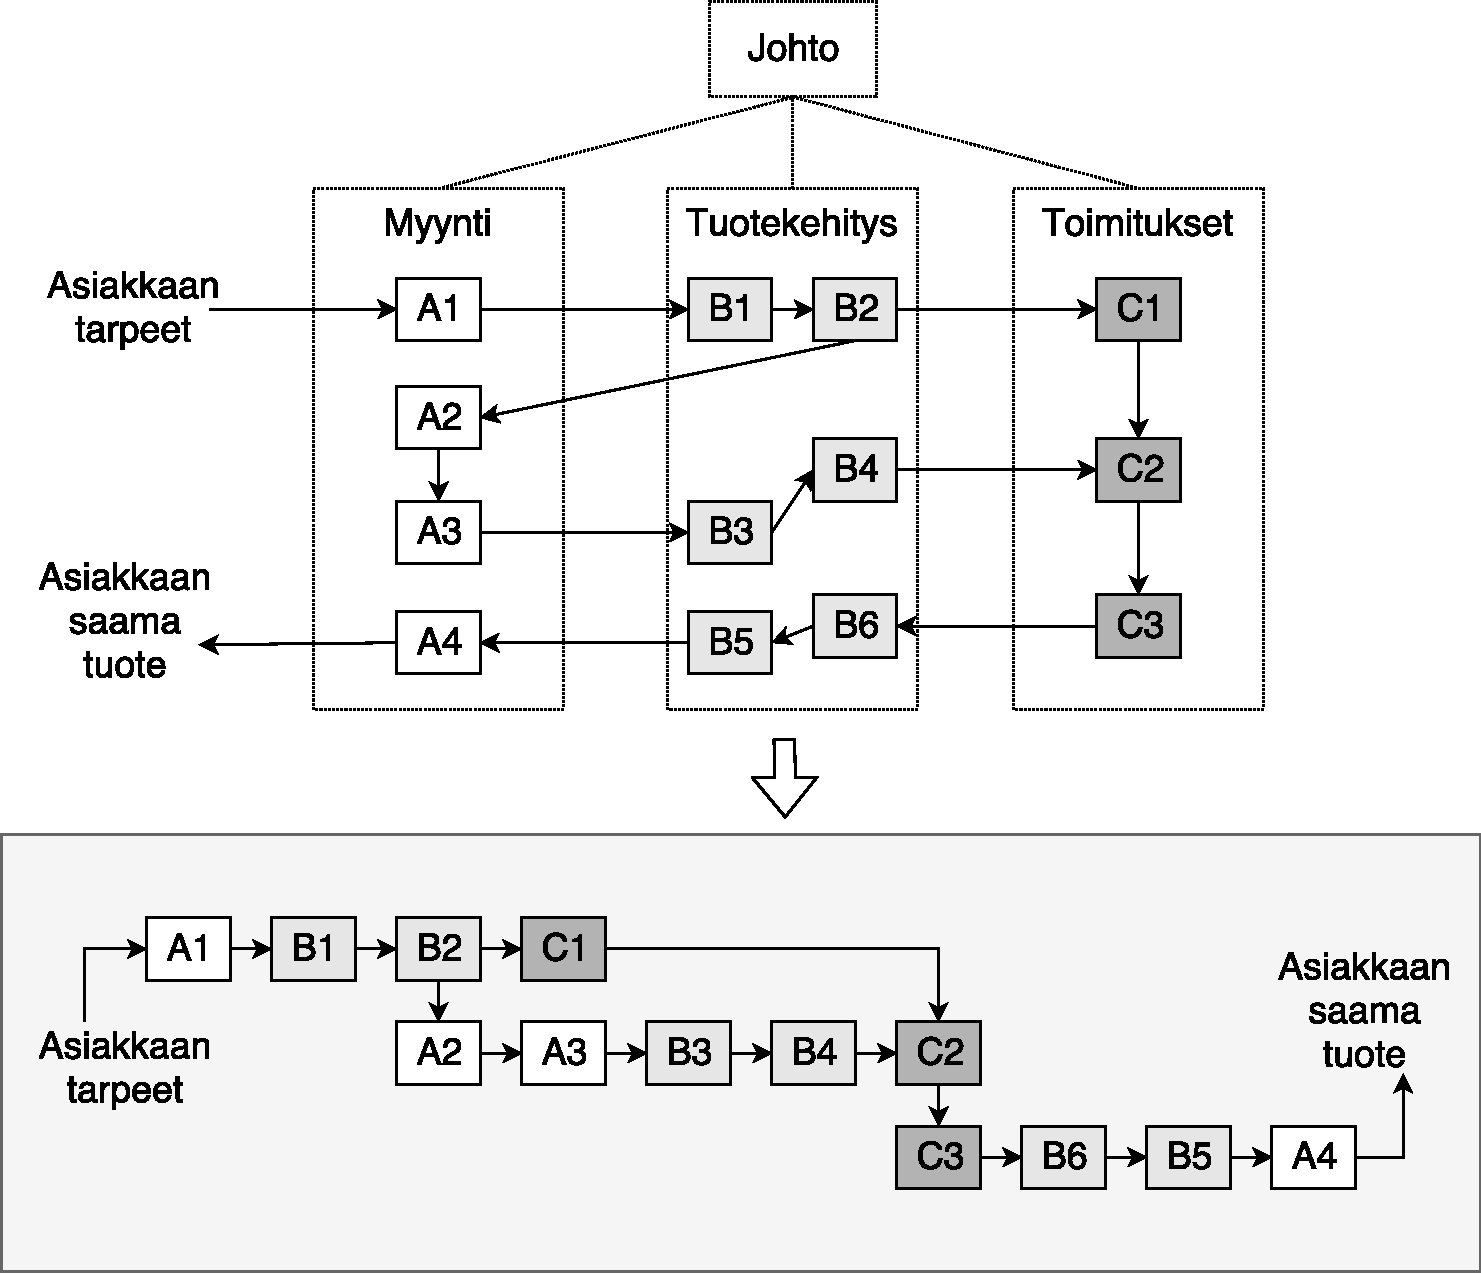
\includegraphics[scale=0.45]{images/Prosessikaavion.pdf}
    \caption{Liiketoimintaprosessin ja organisaatiokaavion yhteys. \citep{ohjelmistotuotanto}}
    \label{fig:liikark}
\end{figure}

Kuvassa \ref{fig:liikark} kuvataan miten liiketoimintaprosessi kulkee ohjelmistoja tuottavan yrityksen toimintojen välillä. Prosessijohtaminen vaikututtaakin yrityksen organisaatiorakenteeseen. On tavallista, että organisaatiorakenne kuvaa yrityksen funktionaalisia toimintoja, kuten myyntiä tai tuotekehitystä. Prosessijohdetussa yrityksessä organisaatiorakenne voidaan kuvata liiketoimintaprosessien mukaisesti, jolloin jokainen prosessi sisältää tarvitsemansa funktionaalisen toiminnon. Useimmilla yrityksillä nämä kaksi organisaatiorakennetta ovat olemassa päällekäin, jolloin yrityksen funktionaaliset toiminnot kuvataan horisontaalisesti ja prosessit vertikaalisesti. \citep{vanhatorre}\\

Liiketoimintaprosessit ja niiden tukiprosessit muodostavat koneiston, jolla yritys toimii. Tästä koneistosta käytetään kirjallisuudessa termiä prosessiarkkitehtuuri, ja sen tehtävä on kuvata miten tämä koneisto toimii ja miten sen sisältämät prosessit liittyvät toisiinsa.\\

Prosessijohtamisessa oletetaan, että organisaation tuottamia palveluita tai tuotteita voidaan kehittää prosesseja kehittämällä. Seuraavassa alaluvussa pureudutaan prosessien mallintamisen rooliin prosessien kehityksessä.

\subsection{Liiketoimintaprosessien mallintaminen}

Liiketoimintaprosessien kehittämisen yksi tärkein lähtökohta on ymmärtää niiden nykytilaa. Nykytilan ymmärtämiseksi liiketoimintaprosesseista luodaan visuaalisia prosessikuvauksia, jossa kuvataan prosessin vaiheita. Tyypillisesti prosessikuvauksessa pyritään tuomaan esiin prosessin eri toimintojen välisten syötteiden, lopputulosten ja informaation kulkua. Prosessikuvauksen tärkein tehtävä on kuvata todellisia toimintamalleja ja toimia viestinnän välineenä prosessin kehityksessä. \citep{ohjelmistotuotanto}\\

Liiketoimintaprosesseja mallinnetaan monitasoisesti prosessijohdetuissa organisaatioissa. Korkealla tasolla mallinnetaan viitekehyksen omaisesti yrityksen tärkeimpiä liiketoimintaprosesseja ja niiden riippuvuussuhteita. Hieman alemmalla tasolla kuvataan yksittäisen prosessin eri vaiheita ja riippuvuuksia toisiin prosesseihin. Alimman tason kuvaukset ovat tarkkoja esityksiä yksittäisen prosessin aktiviteeteista, toimijoista ja informaation kulusta. \citep{teollisuustalous} \\

Tyypillisiä tekniikoita prosessien kuvaamiseen ovat esimerkiksi:

\begin{itemize}
\setlength{\itemsep}{0pt}
    \item Vuokaavio
    \item Tietovirtakaavio
    \item Arvovirtakuvaus
    \item Asiakaspolku
    \item Gantt-kaavio
\end{itemize}

Tämän listan lisäksi on olemassa useita muitakin tapoja ja tekniikoita prosessien kuvaamiseen. Oleellista on valita tavoitetilaa ja käyttötarkoitusta palveleva menetelmä. Viime vuosina suosiotaan ovat nostaneet erityisesti asiakasarvon luontia korostavat ketterät menetelmät, kuten esimerkiksi asiakaspolun kuvaaminen. Näiden menetelmien avulla olennaisten asioiden löytäminen ja viestiminen on koettu olevan perinteisiä menetelmiä tehokkaampaa \citep{lamoureux}. \\

Liiketoimintaprosessin mallintaminen voidaan tehdä esimerkiksi olemassa olevien ohjeistuksien, sidosryhmien haastatteluiden ja fasilitoitujen työpajojen avulla. Prosessin mallintamisessa ja kehittämisessä olennaista on kohdistaa toimenpiteet todellisen toiminnan kehittämiseen, eikä vain mallintamisen ja kehitystoimenpiteiden suunnitteluun. \citep{ohjelmistotuotanto}\\

%Liiketoimintaprosessien mallintaminen nousee tärkeäksi erityisesti prosesseja automatisoidessa.

\subsection{Liiketoimintaprosessien kehittäminen}

Kirjallisuudessa nousee esiin useita eri näkökulmia ja menetelmiä lähtökohdaksi  liiketoimintaprosessien kehittämiseen. Tässä alaluvussa esitellään näistä yleisimmät. Tarkoituksena on antaa kuva miten eri menetelmät vaiheistavat prosessien kehittämistä ja mikä näissä vaiheissa on tärkeä ottaa huomioon. Samalla tuodaan esiin ajatuksia eri mallien taustalla.

%\subsubsection{Esteiden teoria (Theory of Constraints)}

%Esteiden teoria on jatkuvan parantamisen viitekehys, joka keskittyy systeemin suorituskykyä rajoittavien esteiden hallitsemiseen. Sen mukaan jokaisella systeemillä, kuten liiketoimintaprosessilla, on kerrallaan vain yksi este, joka rajoittaa sen suorituskykyä tavoitteeseen nähden. Kun estettä kuormitetaan syntyy sen eteen jonoa tai varasto, jolloin koko systeemin läpimenoaika kasvaa ja suorituskyky heikkenee. \citep{goldratt}\\


%Samalla koko systeemin läpimenoaika tulisi asettaa tämän esteen mukaisesti.
%Teorian mukaan kehitystoimepiteiden priorisoinnissä täytyykin keskittyä merkittävimmän esteen eliminoimiseen, koska vain silloin voidaan parantaa koko systeemin todellista suorituskykyä. Kehitystoimenpiteet muualla kuin merkittävimmässä esteessä ovat teorian mukaan illuusioita, jolla ei ole vaikutusta systeemin todellisen suorituskyvyn parantumiseen. Teoria olettaa, että systeemi ei ole koskaan valmis, vaan kehitettävää löytyy aina. Systeemi ilman esteitä tuottaisikin äärettömän määrän arvoa. \citep{goldratt}\\

%Esteiden teoriassa \citep{goldratt} kuvataan viisi askelta esteen eliminoimiseen:

%\begin{enumerate}
%\setlength{\itemsep}{0pt}
%    \item Esteen identifioiminen.
%    \item Esteen tehostaminen
%    \item Synkronoi systeemi esteen mukaisesti
%    \item Keskity esteen poistamiseen
%    \item Aloita alusta
%\end{enumerate}

%Esteiden teorion hyödyntäminen alkaa esteen identifioimisella, joka on usein hankalin osuus. Yksi tapa löytää este on kuormittaa systeemiä ja mitata mihin jonot tai varastot syntyvät. Systeemin sidosryhmillä on usein hyvinkin erilainen näkemys merkittävimmästä esteestä. Viimeistään silloin kun este on poistettu huomataan oliko se todella merkittävin tavoitteeseen vaikuttava este. \\

%Kun este on identifioitu tulee sen tehokkuus maksimoida. Esteen käyttöaste tulisi maksimoida niin, että aikaa ei hukata sen toimiessa. Toisinsanoen esteen läpimenoaika minimoidaan kohdetamalla olemassa olevat resurssit sen tominnan tehostamiseksi.\\

%Kun esteen käyttöaste on maksimoitu, synkronoidaan systeemin muut osat toimimaan sen tahdissa. Muiden osien tulisi tukea esteen maksimaalista käyttöastetta. Esimerkiksi liiketoimintaprosessiin otetaan tällöin tilauksia vastaan sen hitaimman komponentin mukaisesti.\\

%Esteen identifiomisen, tehostamisen ja systeemin synkronoinnin jälkeen tarkastellaan onko se vielä systeemin tavoitteen kannalta suurin este. Jos on, joudutaan sen poistamiseksi aloittamaan laajemmat toimenpiteet, joiden onnistumiseksi tarvitaan investointeja. Näitä toimenpiteitä jatketaan kunnes este poistuu\\

%Viimeinen vaihe muistuttaa siitä, että kyseessä on jatkuvan kehittämisen sykli. Jos jossain edellisissä vaiheissa onnistutaan poistamaan identifioitu este, tulee siirtyä takaisin etsimään seuraavaa merkittävää estettä.\\

\subsubsection{Laatujohtaminen (Total Quality Management)}

Laatufilosofian mukaan yrityksen tuotteiden ja palveluiden laatu rakentuu sen toimintaprosessien laadusta, jonka vuoksi laatu täytyy suunnitella ja rakennetaa niiden sisälle \citep{teollisuustalous}. Sen juuret ovat toisen maailmansodan jälkeisen suurtuotannon kehityksessä, jossa tarvittiin tehokkaita menetelmiä laadunvalvontaan. Laatuajattelua kuvataan johtamismallina, jossa yrityksen strategisia tavoitteita johdetaan tilastollisen laadun seuraamisen ja ohjaamisen avulla. \\

Perinteisesti laatujohtamisen menetelmiä on hyödynnetty massatuotannossa, mutta nykyään sitä sovelletaan laajasti eri toimintoihin, kuten ohjelmistokehitykseen ja tietotyöhön \citep{ohjelmistotuotanto}. Sen avulla pyritään saavuttamaan entistä tuottavampaa liiketoimintaa kustannustehokkuudella ja voittojen maksimoimisella. Laatujohtamisen yksi merkittävimmistä hyödyistä on korkean laadun ja matalan hintatason yhdistäminen, joka luo merkittävän kilpailuedun \citep{teollisuustalous}.\\

Laatuajattelussa korostuu yrityksen määritelmä laadusta, jonka perusteella toimintaa kehitetään. Moderni laatuajattelu määrittää laadun olevan tuotteen tai palvelun kyky täyttää asiakkaan tarpeet ja odotukset \citep{teollisuustalous}. Tämä asiakaslähtöinen laadun määritelmä vaikuttaa vahvasti yrityksen toiminnan johtamiseen, jossa prosesseja kehitetään asiakkaiden tarpeiden ja siten markkinoiden kilpailutilanteen perusteella. \\

Yrityksen sisällä toimintaa johdetaan laatuajattelun mukaan eri näkökulmasta, jossa sille voidaan asettaa selkeät määreet. Sisäisesti laatu on tuotteen tai palvelun vastaavuus tuotemäärittelyihin ja standardeihin. Näiden avulla voidaan määritellä mitkä liiketoimintaprosessin lopputulokset tai eri vaiheet täyttävät sille asetetut laatuvaatimukset. Kustannustehokkuuden ja voittojen maksimoimiseksi laadun täytyy olla kontrolloitua, eli ei liian hyvää tai huonoa, vaan laatuvaatimuksia vastaavaa. \citep{teollisuustalous}\\

Laadun määritelmää tarkennetaan laatutekijöillä, joilla tarkoitetaan tuotteen tai palvelun ominaisuuksia, jonka perusteella asiakas arvioi laatua. Tämän määritelmän perusteella voidaan asettaa laatuvaatimukset ja prosessien kehityksen suunta. Tavallisesti laatutekijöiden merkitys vaihtelee eri asiakasryhmissä. \citep{teollisuustalous}\\

Laatuajattelun vaikutus liiketoimintaprosessien kehittämiseen tiivistyy kahteen kysymykseen:
\begin{itemize}
\setlength{\itemsep}{0pt}
    \item Luoko tominto lisäarvoa, josta asiakas on valmis maksamaan?
    \item Toimiiko prosessi siten, että se maksimoi asiakkaan saaman arvon ja minimoi resurssien käytön?
\end{itemize}

Laatuajattelussa korostuu asiakaslähtöisyys, henkilöstön sitouttaminen ja kouluttaminen sekä laadun jatkuva parantaminen \citep{teollisuustalous}. Laatuajattelun yksi kehittämismalli on PDCA-sykli, jota kutsutaan myös laatuympyräksi. Se koostuu neljästä vaiheesta, jotka toistetaan jatkuvassa syklissä: \\

\begin{itemize}
\setlength{\itemsep}{0pt}
    \item Suunnittele (Plan)
    \item Toteuta (Do)
    \item Tarkista (Check)
    \item Kehitä (Act)
\end{itemize}

Suunnitteluvaiheessa varmistetaan, että prosessin toiminta on standardisoitua, vakiintunutta ja dokumentoitua ennen kehitystoimenpiteiden aloittamista. Tämän jälkeen toimintaa analysoidaan sopivilla menetelmillä, jonka pohjalta määritetään liiketoimintaongelma, dokumentoidaan relevantit ongelmaan vaikuttavat tekijät ja selvitetään ongelmien juurisyyt. Tuloksena syntyy kattavasti dokumentoitu suunnitelma toiminnan kehittämiseksi. \citep{teollisuustalous, mohapatra} \\

Toteutusvaiheessa määritetään mittarit, joilla arvioidaan kehitystoimenpiteiden vaikutusta ongelmaan, ja toteutetaan muutokset. Toteutusvaiheen tuloksena suunnitteluvaiheen dokumentaatioon päivitetään tiedot tehdyistä toimenpiteistä ja mittareista. \citep{teollisuustalous, mohapatra}\\

Tarkistusvaiheessa uudistettujen toimintamallien tulokset käydään läpi ennen ja jälkeen kun se on otettu käyttöön, ja tuloksia analysoidaan valittujen mittareiden perusteella \citep{teollisuustalous}. \\

Kehitysvaiheessa arvioidaan saavutettiinko kehitystoimenpiteillä haluttu lopputulos. Tuloksien dokumentointimalli standardoidaan ja opitut asiat viestitään muille, jotka voivat hyötyä tuloksista. Jos tavoitteet jäivät saavuttamatta, tilanne analysoidaan ja kehityssykli aloitetaan alusta.\citep{teollisuustalous}

\subsubsection{Lean-ajattelu prosessijohtamisessa}

Laatuajattelun pohjalta syntynyt soveltamistapa organisaation toiminnan kehittämiseksi on Lean-ajattelu, jota kuvataan asiakaslähtöiseksi prosessijohtamisen malliksi. Sen juuret ovat fyysisten tuotteiden massatuotannossa, mutta sen periaatteita hyödynnetään laajasti eri toimialoilla. Lean-ajattelua hyödyntävä organisaatio pyrkii tuottamaan asiakkaalle parasta mahdollista arvoa tehokkaalla resurssien käytöllä, jolloin keskitytään yksittäisten asioiden sijaan kokonaisuuden parantamiseen. \citep{leanit}\\

Lean-ajattelussa puhutaan prosessin sijaan arvovirrasta, joka koostuu erilaisista työvaiheista. Jokaiseen työvaiheeseen kuluu aikaa ja resursseja. Työvaiheiden suorittamiseen kulunut aika lasketaan yhteen, jolloin saadaan arvovirran läpimenoaika. Kulunut aika jaetaan kahteen kategoriaan: Arvoa tuottavaan ja ei arvoa tuottavaan. Arvoa tuottava ajalla tarkoitetaan yksinkertaisesti aikaa, joka kului niiden toimenpiteiden suorittamiseen, joiden lopputuloksesta asiakas on valmis maksamaan. Ei arvoa tuottava aika on taas tämän vastakohta. Läpimenoajan ja arvoa tuottavavan ajan suhdetta kutsutaan virtaustehokkuudeksi, joka halutaan maksimoida eliminoimalla ei arvoa tuottavaa aikaa, eli turhuutta tai hukkaa. \citep{leanthinking}\\

Hukkaa tai turhuutta ovat kaikki ihmisen tai koneen toiminta, joka sitoo resursseja mutta ei tuota arvoa. Näistä esimerkkejä ovat \citep{leanthinking}:
\begin{itemize}
\setlength{\itemsep}{0pt}
    \item Virheet joita täytyy toistuvasti korjata puutteellisen toimintamallin vuoksi.
    \item Asioiden tai informaation tuottamista, joita ei tarvita tai jotka kasautuvat varastoksi odottamaan jalostamista.
    \item Prosessointivaiheet joita ei oikeasti tarvita, vaikka niin olisi totuttu tekemään.
    \item Työntekijöiden tarpeeton liikkuminen paikasta toiseen.
    \item Materiaalin tai informaation kuljettaminen paikasta toiseen ilman tarkoitusta
    \item Aikaisemman työnvaiheen tuloksen odottelu oman työn aloittamiseksi.
    \item Tuotteiden tai palveluiden tuottaminen, jotka eivät kohtaa asiakkaiden tarpeita ja ovat siten virhellisiä.
\end{itemize}

Hukan eliminoimiseksi Lean-ajattelu noudattaa viittä periaatetta, jotka on listattu alle:

\begin{enumerate}
\setlength{\itemsep}{0pt}
    \item Arvon määritteleminen
    \item Arvivirran kartoittaminen ja kuvaaminen
    \item Arvovirran läpimenoajan minimointi
    \item Arvovirran imuohjaus
    \item Arvovirran jatkuvan kehittäminen
\end{enumerate}

 Ensimmäinen vaihe on kriittisimmän komponentin eli arvon määrittäminen, jonka voi ainoastaan tehdä asiakas. Arvon määritelmä paljastaa mikä oikeasti on hukkaa ja mikä tuottaa arvoa. Joskus asiakkaan voi olla vaikea kuvailla tyhjentävästi mikä oikeasti on hänelle arvokasta. Siksi onkin tärkeä käyttää useita erilaisia metodeja samanaikaisesti, että voidaan selvittää mitä asiakas haluaa, miten hän haluaa tuotteen tai palvelun, mihin hintaan ja koska. Usein arvon määrittäminen onkin hankalaa, koska sitä voi olla vaikea kuvailla tai selvittää ja siitä saattaa olla useita erilaisia käsityksiä. \\

Kun arvosta on olemassa riittävän hyvä määritelmä on tarkoituksen mukaista kartoittaa kaikki toimenpiteet joita vaaditaan sen tuottamiseksi. Kyseessä on toinen periaate, eli arvovirran kartoittaminen josta muodostetaan arvovirtakuvaus. Sen tavoite on määrittää jokaiselle tuotteelle tai palvelulle ne toimenpiteet, joiden tuloksena syntyy asiakkaan vaatimukset täyttävä lopputulos. Tyypillisesti arvoketju koostuu erilaisista ongelmanratkaisua, informaationhallintaa ja raaka-aineiden jalostamista sisältävistä toimenpiteistä. Nämä erilaiset toimenpiteet voidaan arvon määritelmän mukaisesti jakaa kolmeen kategoriaan. Useat toimenpiteet yksiselitteisesti luovat arvoa. Toiset selkeästi eivät tuota arvoa, mutta ovat teknisten tai toiminnallisten olosuhteiden pakosta välttämättömiä. Sitten on selkeästi ei arvoa tuottavia toimenpiteitä, joiden eliminoimiseen tulisi keskittyä. Ratkaisevaa on kaikkien toimenpiteiden tekeminen läpinäkyväksi, jolloin on syvällinen ymmärrys siitä miten arvovirrassa olevaa työtä tehdään.\\

Kolmannen periaatteen mukaan, kun eliminoitavaksi kelpaavat toimenpiteet on poistettu, keskitytään arvovirran läpimenoajan lyhentämiseen. Tarkoituksena on pitää arvovirta koko ajan liikkeellä pienissä erissä vain asiakastarpeen mukaan ohuena jatkuvana nauhana. Arvovirran toimenpiteet sijaitsevat tavallisesti useissa organisaatioyksiköissä, joissa ajaudutaan usein optimoimaan työtä omasta näkökulmasta. Tällöin arvovirran läpimeno muistuttaa katkeilevaa paksua ja epätasaista janaa, jossa katkeaminen edustaa odottamista. Jokaiseen toimenpiteeseen kuluva aika jakautuu odotusaikaan ja prosessointiaikaan. Tarkoituksena tässä vaiheessa on minimoida jokaisen toimenpiteen odotusaika tekemällä työtä pienissä erissä, jolloin vältetään välivarastojen ja jonojen muodostuminen, jotka aiheuttavat odotusajan. Tälläistä arvovirran läpimenoa kutsutaan imuohjaukseksi, ja onnistuessaan se johtaa nopeaan tuotekehitys- ja toimitussykliin.\\

Neljännen periaatteen mukaan imuohjaus johtaa organisaation nopeaan kykyyn vastata asiakkaan tarpeisiin, jolloin voidaan unohtaa myyntiennusteiden tekeminen ja keskittyä asiakastarpeeseen vastaamiseen. Imuohjauksen taustalla on ajatus siitä, että välivarastot aiheuttavat kustannuksia ja tekevät prosesseissa olevat ongelmat näkymättömiksi.\\

Viides periaate hakee täydellisyyttä jatkuvalla kehittymisellä, joka tulee osaksi organisaation kulttuuria. Periaatteen tavoite on ymmärtää, että hukkaa tai turhuutta löytyy aina lisää, joten kokonaisuutta tulisi yksinkertaistaa jatkuvissa nopeissa kehityssykleissä aikaisempien periaatteiden mukaisesti.\\

%“lean thinking” is a practice which considers the expenditure of assets and resources for any goal other than the creation of value for the end customer to be wasteful. These wasteful practices or business processes (which are not yet optimized) are therefore a clear target for elimination. Hence, at the most essential level, “lean” is centered on preserving value with less work.

%In our presentations to industrial audiences, we often point out that the
%only sure thing about forecasts is that they are wrong. (Which is why lean
%thinkers strive to reduce order-to-delivery times to such an extent that most
%products can be made to order and always try to add or subtract capacity
%in small increments.)

\subsubsection{Liiketoimintaprosessin uudistaminen (Business Process Reengineering)}

Joissain tapauksissa on tarkoituksen mukaista harkita liiketoimintaprosessin uudistamista jatkuvien pienempien kehitysaskelten sijaan. Sen taustalla on 1990-luvulla yleistynyt laatuajattelun yleistyminen, jonka vuoksi kilpailussa pärjäämiseen tarvittiin nopeampia keinoja kuin olemassa olevien liiketoimintaprosessien osittainen kehittäminen. Liiketoimintaprosessien uudistamisessa on seuraavia keskeisiä ominaisuuksia \citep{mohapatra}:

\begin{itemize}
\setlength{\itemsep}{0pt}
    \item Radikaali muutos vanhaan.
    \item Yrityksen toiminnan suunta muuttuu.
    \item Liiketoimintaprosessit uudistetaan lähes täysin.
    \item Yrityksen organisaatiomalli muuttuu.
    \item Teknologisilla parannuksilla tuetaan muutosta.
    \item Tavoitteena on asiakaskokemuksen parantaminen ja toiminnan kustannustason laskeminen.
\end{itemize}

Liiketoimintaprosessien uudistamisen tarve nähdään syntyvän olemassa olevien prosessien osittaisen kehittämisen tuomasta harhasta, jossa arvoa tuottamatonta työtä ei pystytä hävittämään tarpeeksi tehokkaasti. Tästä esimerkkinä on teknologian hyödyntäminen vain arvoa tuottamattoman työn automatisoimiseen, kun työ voitaisiin hävittää kokonaan ja investoinnit teknologiaan voitaisiin kohdentaa vahvemmin arvoa tuottavan työn kehittämiseen. \citep{hammer}\\

Liiketoimintaprosessien uudistaminen keskittyy strategisiin ja lisäarvoa tuottaviin tärkeimipiin organisaation prosesseihin, jotka ulottuvat organisaation rajojen ulkopuolelle. Sen avulla on mahdollista saavuttaa liiketoiminnallisesti isompia tuloksia, mutta vaatii isomman investoinnin korkeammalla riskillä kuin muut metodit. Tämän vuoksi on kriittistä saavuttaa johdon täysi tuki sen läpivientiin.\\

Uudistamisprosessissa on neljä vaihetta, joiden perusteella prosessien uudistamista suorittava organisaatio määrittelee tarkemmat askeleet sen tarpeiden mukaan: \citep{mohapatra}

\begin{itemize}
\setlength{\itemsep}{0pt}
    \item Identifioi prosessit
    \item Analysoi prosessit
    \item Suunnittele tavoitetilan ominaisuudet
    \item Toteuta ja testaa uusi prosessi
\end{itemize}

Ensimmäisessä vaiheessa identifioidaan nykyiset prosessit mahdollisimman kattavasti. Toisessa vaiheessa ne analysoidaan ja nostetaan esiin strategisesti tärkeimmät prosessit, joihin toimenpiteet tulisi kohdistaa. Tämän jälkeen suunnitellaan tavoitetilan ominaisuudet, joita kehitetään valittuihin prosesseihin. Tämän perusteella organisaatio tietää mihin sen tulee päästä uudistamistyössä ja mitä sen tulee saavuttaa. Viimeisessä vaiheessa toteutetaan uudistustyö suunnitelman perusteella ja kehitetään sitä jatkuvasti. \citep{mohapatra}\\

\subsubsection{Kypsyysmallit}

Kypsyysmallissa ajatellaan, että organisaation kypsyys tai maturiteetti määrää sen suorituskyvyn. Kypsyysarviointi mittaa organisaation kykyä käyttää hyödyksi sen prosesseja, ihmisiä, työkaluja, tuotteita ja johtamista. Arvio esittää miten organisaatio suoriutuu kilpailijoihinsa nähden, ja kannustaa jatkuvaan johtamisen ja prosessien kehittämiseen. \citep{mohapatra}\\

Useimmissa kypsyysmalleissa on viisi tasoa, ja mitä korkeampi taso sitä kyvykkäämpi organisaatio on kyseessä. Mallia voi hyödyntää joko yhteen, useampaan tai kaikkiin organisaation prosesseihin. Perinteisesti matalan kypsyystason organisaation on kannattava aloittaa kehitys yhdestä ja tärkeimmästä prosessista. \citep{mohapatra}

\begin{itemize}
\setlength{\itemsep}{0pt}
    \item Taso 1: Alkutilanne, jossa käytetyt toimintamallit riippuvat toteuttajasta, eli toistettavia prosesseja ei ole.
    \item Taso 2: Toistettavia prosesseja, aikaisempi onnistuminen voidaan toistaa.
    \item Taso 3: Määrämuotoiset prosessit, jotka on määritelty tavoitteiden perusteella, ja niitä noudatetaan ja pyritään kehittämään.
    \item Taso 4: Mitattavat prosessit, eli toimintaa kyetään mittaamaan ja tuloksia käytetään käyttämään toiminnan parantamiseksi.
    \item Taso 5: Optimoidut prosessit, mittaukset ovat automaattisia, ja tuloksia hyödynnetään tehokkaasti kokonaisuuden optimointiin.
\end{itemize}

Kypsyysmallin käytössä pyritään ensin selvittämään oma taso, jonka jälkeen suoritetaan kehitystoimenpiteitä kypsyystason nostamiseksi. Malli tarjoaa järjestyksen mitä ominaisuuksia organisaation toiminnassa tulisi ensin kehittää. \citep{okaytannot} \\

%\subsubsection{Laaja liiketoimintaprosessien kehittämismalli (Business Process Management)}

%Weske argues that all communities involved need to have a common understanding of the different aspects of business process management. To this end, he details the complete business process lifecycle from the modeling phase to process enactment and improvement, taking into account all different stakeholders involved. 

%Laajassa liiketoimintaprosessien kehittämismallissa korostetaan jatkuvan prosessien kehittämisen merkitystä organisaation johtamisessa, ja kypsyysmallin soveltamista kehityspoluksi. Sen taustalla on erilaiset liikkeenjohdon ja tietotekniikan hyväksi havaitut toimintamallit. Kehittämismalli tarjoaa viitekehyksen, jonka perusteella voidaan arvioida organisaation prosessijohtamista, ja ohjata kehitystä toimintoihin keskittyneestä organisaatiomallista prosessikeskeiseen organisaatiomalliin. Mallin kuvaus korostaa, että kaikilla kehityksessä mukana olevilla sidosryhmillä on oltava yhteinen jaettu ymmärrys liiketoimintaprosessien kehittämisestä. Muutoksessa onnistumisen takaa vain tiivis organisaatiorajoista riippumaton yhteistyö, joka johtaa myös kulttuurisiin muutoksiin. \citep{weske}\\

%Liiketoimintaprosessien kehittämistä lähestytään kahdesta näkökulmasta: Liikkeejohdon ja tietotekniikan näkökulmista, jotka on saatava toimimaan yhdessä. Liikkeenjohto tavoittelee yrityksen suorituskyvyn parantamista kehittämällä asiakastyytyväisyyttä, kustannustehokkuutta ja uusien tuotteiden ja palveluiden tuottamista pienillä kustannuksilla. Teknologiasta vastaavat taas tavoittelevat lujatekoisten ja skaalautuvien tietojärjestelmien tuottamista. Nämä kaksi näkökulmaa eivät sovi automaattisesti yhteen, mutta ovat vahvasti riippuvaisia toisistaan. Laaja liiketoimintaprosessin kehittämismalli pyrkii tuomaan nämä kaksi näkökulmaa saman viitekehyksen sisälle. \citep{weske}\\

%Kehittämismallissa koostetaan toimintamalleja ja työkaluja, joiden avulla tuetaan liiketoimintaprosessien suunnittelua, hallitsemista, kokoonpanoa, kehittämistä, analysointia ja automatisointia. Mallin pohjana on ymmärrys organisaation eri toiminnoista, tietojärjestelmistä ja näiden välistä riippuvuussuhteista. Riippuvuussuhteet esitetään määriteltyinä liiketoimintaprosesseina, joita voidaan analysoida ja kehittää suhteessa organisaation strategisiin tavoitteisiin. \citep{weske}\\

%Lisäksi todetaan, että yrityksen kannalta on hyödyllistä käyttää liiketoimintaprosessin toimintoja ohjaavaa tietojärjestelmää. Järjestelmän avulla voidaan seurata prosessien läpimenoja, kerätä lokitietoa, havainnoida mahdollisia kehityskohteita ja huomata mahdolliset laatupoikkeamat niiden lähteellä. \citep{weske}\\

%Kehittämismallissa jaetaan liiketoimintaprosessien kehityksen elinkaari neljään vaiheeseen:

%\begin{enumerate}
%\setlength{\itemsep}{0pt}
%    \item Analysointi ja suunnittelu
%    \item Konfigurointi
%    \item Ylläpito
%    \item Arviointi
%\end{enumerate}

%Analysointi ja suunnitteluvaiheessa kartoitetaan liiketoimintaprosesseja ja niiden toiminallisia ja teknisiä olosuhteita. Kartoituksen perusteella suunnitellaan toteutettavat liiketoimintaprosessit ja tehdään niistä visuaalinen malli. Visuaaliset mallit toimivat kommunikoinnin työvälineinä prosesikehitystä suorittaville sidosryhmille. Mallintamiseen voidaan käyttää erilaisia tekniikoita riippuen sovelluskohteesta ja abstraktion tasosta. Mallintamisen jälkeen ne validoidaan yhdessä sidosryhmien kanssa, esimerkiksi mallia simuloivassa työpajassa. \\

%Konfigurointivaiheessa mallinnettu liiketoimintaprosessi tuodaan käytäntöön. Tämä vaihe vaatii uusien ohjeistuksien luomista ja kouluttamista prosessissa toimiville henkilöille ja käytettyjen tietojärjestelmäratkaisujen valintaa ja toimeenpanoa. Tämän jälkeen testataan liiketoimintaprosessin toimintaa käytännössä, ja havaitut puutteet korjataan ennen käyttöönottoa.\\

% seurataan liiketoimintaprosessia käytännössä. Tässä vaiheessa huomio kiinnitetään jokaisen prosessin läpimenon monitorointiin varmistaen, että sen aktiviteetit toimivat suunnitellusti. Monitoroinnissa on hyödyllistä käyttää visuaalisia mallinnuksia, joista selviää lähes reaaliajassa käynnissä oleva vaihe. Tässä vaiheessa myös kerätään tarkää lokitietoa, joka toimii syötteenä arviointivaiheeseen.\\

%Arviointivaiheessa käytetään kerättyä tietoa ja sitä hyödyksi käyttäen arvioidaan onko liiketoimintaprosessi tavoitetilassa. Arvioinnissa reflektoidaan myös miten aikaisemmissa vaiheissa on onnistuttu, ja tehdään mahdollisia parannuksia. Arvioinnin jälkeen voidaan taas aloittaa alusta.\\




%Monitorointivaiheessa seurataan liiketoimintaprosessin toimintaa käytönnössä. 


%käyttää liiketoimintaprosessien elinkaaren kuvausta kehittämismallin ymmärtämiseen.

%Elinkaari koostuu toisiinsa liittyvistä vaiheista, jotka toistuvat iteratiivisesti. 

%Vaiheet järjestetään syklisessä rakenteessa,
%mikä osoittaa niiden loogiset riippuvuudet.

%The business process lifecycle is shown in Figure 1.5; it consists of phases
%that are related to each other. The phases are organized in a cyclical structure,
%showing their logical dependencies. These dependencies do not imply a strict
%temporal ordering in which the phases need to be executed. Many design
%and development activities are conducted during each of these phases, and
%incremental and evolutionary approaches involving concurrent activities in
%multiple phases are not uncommon.


%Traditionally, business processes are enacted manually, guided by the
%knowledge of the company’s personnel and assisted by the organizational regulations
%and procedures that are installed.
%Enterprises can achieve additional benefits if they use software systems
%for coordinating the activities involved in business processes. These software
%systems are called business process management systems.


%recappaa se intro





%Laaja kehittämismalli on vahvasti sidoksissä tietojärjestelmien hyödyntämiseen prosessien kehittämisessä. tarkkoja prosessikuvia...

%The most recent trends in BPM are influenced by the emergence of cloud technology, the prevalence of social media, mobile technology, and the development of analytical techniques. Cloud-based technologies allow companies to purchase resources quickly and as required independent of their location. Social media, websites and smart phones are the newest channels through which organizations reach and support their customers. The abundance of customer data collected through these channels as well as through call center interactions, emails, voice calls, and customer surveys has led to a huge growth in data analytics which in turn is utilized for performance management and improving the ways in which the company services its customers.


\subsubsection{Yhteenveto liiketoimintaprosessien kehittämisestä}

%Business process management is based on the observation that each product that a company provides to the market is the outcome of a number of activities performed.

Yhteenvetona voidaan todeta, että liiketoimintaprosesseja on mahdollista kehittää monesta eri näkökulmasta. Jokaisen tavoitteena on parantaa liiketoimintaprosessin suorituskykyä, joko tehostamalla, eliminoimalla tai automatisoimalla sen sisältämiä toimintoja. Suorituskyky kasvaa joko läpimenoajan lyhentymisellä, kustannustehokkuudella tai tuottamalla asiakkaan kannalta arvokkaampia lopputuloksia. Suorituskyky on siis optimointia, joka tuottaa parhaan mahdollisen lopputuloksen mahdollisimman pienillä resursseilla. \\

Eri lähestymistavat toivat myös esiin, että kehittäminen on jatkuvaa syklistä toimintaa, jolla varmistetaan yrityksen valmiudet kilpailla markkinoilla. Jatkuva kehittäminen on seurausta olosuhteiden jatkuvasta muuttumisesta. Asiakkaiden tarpeet muuttuvat ja markkinoilla toimivat kilpailujat tehostavat omia liiketomintaprosessejaan ja ottavat käyttöön uusia teknologioita.\\

Jokaisella lähestymistavalla on oma painotuksensa, mutta kaikki jakavat kehittämisen toimenpiteet vaiheihiin joiden mukaan edetään. Liiketoimintaprosessien kehittämisen eri lähestymistapojen perustana voidaan nähdä ymmärrys nykytilasta, tavoitetilasta ja näiden kahden tilan erojen tunnistamisesta. Kun näiden kahden tilan väliset erottavat tekijät on tunnistettu, pystytään priorisoimaan kehitystä vaativat osa-alueet. Nykytilan ymmärtäminen tarkoittaa prosessiketjun todellisten toimintamallien tuntemista, jolloin voidaan nähdä prosessin eri vaiheiden vaikutus lopputulokseen ja priorisoida missä järjestyksessä niihin halutaan vaikuttaa. Tavoitetila on kuvaus niistä ominaisuuksista tai laatuvaatimuksista, jotka ohjaavat prosessin kehittämisen toimenpiteitä.\\

Kehittämismalleissa tuotiin esiin, että kehittämisessä voidaan keskittyä yksittäisiin tai useampaan prosessiin kerralla. Huomio on kuitenkin tarkoitus kiinnittää yrityksen kannalta tärkeimpiin liiketoimintaprosesseihin tai niiden vaiheisiin, joihin vaikuttamalla saadaan kokonaisuuden kannalta myönteisimpiä muutoksia aikaan.\\



%sen tavoitteena on kasvattaa yrityksen suorituskykyä markkinoilla. Liiketoimintaprosessin suorituskykyä voidaan kasvattaa sen sisältämiä toimintoja tehostamalla, eliminoimalla ja automatisoimalla, jolloin kustannukset ja läpimenoaika laskevat tai asiakkaan saama arvo lisääntyy. Tavoitteena on siis tuottaa paras mahdollinen lopputulos mahdollisimman pienillä resursseilla. Resursseja ovat esimerkiksi aika, raha, materiaalit ja työvoima. \\%\citep{leanit} \\

%Eri kehittämismallit toivat esiin, että ajan kuluessa asiakkaiden tarpeet muuttuvat ja markkinoilla toimivat kilpailijat kehittävät liiketoimintaprosessejaan yhä paremmiksi. Siksi liiketoimintaprosessien kehittämisen on oltava jatkuvaa tomintaa, jolla varmistetaan yrityksen valmiudet vastata muuttuviin asiakastarpeisiin ja säilymään kilpailukykyisenä markkinoilla. Edellytyksenä kuitenkin on prosessikulttuurin olemassaolo, jolloin voidaan olettaa toiminnan perustuvan prosessien käyttöön, mittaamiseen ja niiden avulla johtamiseen. \citep{teollisuustalous}\\

%Prosessien kehityksessä huomio kiinnitetään yrityksen kannalta tärkeimpiin arvoa tuottaviin prosesseihin. Tällöin prosessille vastuutettu omistaja on vastuussa kehittämistoimenpiteistä. Liiketoimintaprosessien kehittämisen lähtökohtana on ymmärrys nykytilasta, tavoitetilasta ja näiden kahden tilan erojen tunnistamisesta. Kun näiden kahden tilan väliset erottavat tekijät on tunnistettu, pystytään priorisoimaan kehitystä vaativat osa-alueet. Nykytilan ymmärtäminen tarkoittaa prosessiketjun todellisten toimintamallien tuntemista, jolloin voidaan nähdä arvoa tuottavat ja tuottamattomat vaiheet. Tavoitetila on kuvaus niistä ominaisuuksista tai laatuvaatimuksista, jotka ohjaavat prosessin kehittämisen toimenpiteitä. \citep{leanit}\\


\subsection{Liiketoimintaprosessin automatisoiminen}

Monilla aloilla menestyksen perusedellytyksenä on tehokkaan automaation soveltaminen liiketoimintaprosesseissa \citep{teollisuustalous}. Automaatio on tulosta prosessien jatkuvasta kehityksestä, jossa kasvanut ymmärrys nykyisistä toimintamalleista ja niiden suhteesta tulokseen onnistutaan yhdistämään organisaatiolle sopivan teknologian parhaisiin käytäntöihin \citep{clarkin}. 

%liiketoiminnan tavoitteista, ihmisen roolista prosessissa ja soveltuvista teknologiosta yhdistetään optimoiduksi kokonaisuudeksi.

%, jolloin onnistutaan muodostamaan määrämuotoisia ja toistuvia toimintamalleja arvon tuottamiseen, . 

%Automaatiolla voidaan osittain korvata työvoimaa ja pienentää tätä kautta liiketoiminnan kustannuksia. Jatkuva teknologinen kehitys edesauttaa automaation yleistymistä yhä monimutkaisemmissa sovelluksissa \citep{mohapatra}.

\subsubsection{Automaation määritelmä}

Automaatio on mekaaninen tai tietotekninen työkalu ihmisten aikaisemmin suorittamiin tehtäviin, ja yhä enemmän tehtäviin jotka olisivat muuten mahdottomia. Automaatiossa ihmisen luomat koneet integroituvat itsenäisesti toimivaksi järjestelmäksi, joka ei vaadi ihmisen väliintuloa ajon aikana. Automaattinen järjestelmä suorittaa prosessia sen saamien tarkkojen ohjeiden mukaisesti, ja ohjeiden noudattamista valvoo palautekontrolli, jonka tehtävä on validoida järjestelmään tulevien syötteiden oikeellisuus ja valvoa ohjeiden noudattamista prosessin aikana. \citep{groover} \\

Automaation hyödyt voidaan tiivistää seuraavasti \citep{groover, teollisuustalous}:

\begin{itemize}
\setlength{\itemsep}{0pt}
    \item Työn tuottavuuden kasvu
    \item Tasainen laatu
    \item Nopea läpimenoaika
    \item Korkeampi käyttöaste
\end{itemize}

Ihmisen manuaalisesti tekemään työhön verrattuna automaattinen järjestelmä kykenee työskentelemään kellon ympäri seitsemänä päivänä viikossa, jolloin käyttöaste ja työn tuottavuus korkea. Se myös tekee työtä tarkasti sen saamien ohjeiden mukaan, jolloin vältytään manuaalisille työvaiheille tyypillisistä virheistä tai laadun vaihtelusta. Kone myös tekee tarkuutta ja huolellisuutta vaativan työn selkeästi nopeammin kuin ihminen. \citep{groover}\\

Automaation haitat voidaan tiivistää seuraavasti:

\begin{itemize}
\setlength{\itemsep}{0pt}
    \item Työntekijöiden irtisanominen
    \item Korkeat investoinnit
    \item Virheiden suurentuminen
    \item Teknologiset ja taloudelliset riskit
    \item Vaatii uutta osaamista
\end{itemize}

Suurimmaksi automaation haitaksi nähdään pienempi tarve työvoimalle, jolloin useat työntekijät voivat menettää työnsä. Automaatio on perinteisesti luonut uusia työpaikkoja, mutta ne eivät välttämättä ole sopivia irtisanotuille tai vaativat uudelleen kouluttautumista. Automaation rakentaminen vaatii poikkeuksetta investointia, jonka vaatii jatkuvaa ylläpitoa ja se joustaa muutostilanteissa selkeästi ihmistä heikommin. Jos automaatiolle antaa virheellisiä ohjeita, se korostaa virhettä läpi prosessin. \citep{groover}\\

\subsubsection{Automaatio liiketoimintaprosesseissa}

%Liiketoimintaprosessien automatisoinnissa yhdistyy organisaation strategia, ihmisen rooli prosessin tukena, automaattisen prosessimallin luominen ja tarkoitukseen sopivan teknologian hyödyntäminen. Prosessien automatisointi on jatkuvaa kehitystä, jota ohjaa liiketoiminnalliset tavoitteet.\\

Liiketoimintaprosessin automaatiolla tarkotetaan tietokoneavusteista resurssien, laitteiston ja ihmisen tietämyksen koordinointia optimoiduksi kokonaisuudeksi, joka tuottaa halutun lopputuloksen. Haluttuun lopputulokseen saavuttaminen on pääasiassa prosessin jatkuvaa optimointia, jonka tuloksena voidaan hyödyntää erilaisia teknologisia ratkaisuja soveltuvien prosessin osien automatisointiin.  \citep{mohapatra}\\

Yrityksen haasteena prosessin automatisoimisessa on ensin kärsivällisesti virtaviivaistaa ja suunnitella uusi prosessimalli, jolloin vältetään turhien prosessin vaiheiden automatisoiminen \citep{mohapatra}. Onkin huomattavasti tehokkaampaa eliminoida arvoa tuottamaton työ, kuin haaskata resursseja sen automatisoimiseen. Automaation soveltamista tulisikin harkita tarkkaan, koska se moninkertaistaa sovelluskohteensa lopputuloksen, oli se sitten arvoa tuottavaa tai ei. \citep{hammer}\\

Automaation hyödyntämisen lähtee liiketoiminnallisesta perustasta, joka on lähtöisin organisaation tavoitteista, eikä esimerkiksi jo tehdyistä teknologisista valinnoista. Liiketoiminnan näkökulma määrittää ja rajaa ongelman, joka sitten ratkaistaan teknologisesta näkökulmasta. \citep{mohapatra}\\

Ihmisen rooli täytyy myös nähdä automaation mahdollistajana, eikä vain tukena \citep{mohapatra}. Ihmisen vahvuudet ovat luovassa ongelmanratkaisussa, eikä toistuvien työvaiheiden suorittamisessa. Siksi automaation tulisikin hoitaa rutiininomaiset tehtävät ja tukea ihmistä tarjoamalla luotettavaa tietoa luovien ratkaisujen tueksi \citep{leanit}.\\

Liiketoimintaprosessien automatisoinnissa ratkaistavat ongelmat liittyvät usein prosessin aikaa vievien ongelmien eliminoimiseen, kuten päätöksenteon hitauteen, tiedon puutteeseen tai virheellisyyteen. Automaatioratkaisuissa tieto tulee sisään yhdestä määrätystä pisteestä, ja tiedon oikeellisuutta validoidaan ja monitoroidaan. Tiedonkulun ollessa stanrardoitua ja luotettavaa, prosessin toimijat voivat tehdä päätöksiä itsenäisesti ja nopeasti. \citep{mohapatra}\\

Liiketoimintaprosessien automatisointi onkin ensisijaisesti mahdollisuus yksinkertaistaa työnkulkua ja eliminoida turhia työvaiheita. \citep{mohapatra}\\

\subsubsection{Automatisoinnin lähtökohdat}
 
Kirjallisuudesta nousee esiin seuraavia ominaisuuksia, joiden avulla tulisi lähestyä prosessin automatisointia:

\begin{itemize}
\setlength{\itemsep}{0pt}
    \item Selkeän liiketoiminnallisen tavoitteen määrittäminen ja rajaus
    \item Tärkeimpien sidosryhmien tuki
    \item Sopivan prosessin valitseminen
    \item Pienet kehityssyklit isojen hankkeiden sijaan
    \item Sopivan teknologian hyödyntäminen
\end{itemize}

Tarkkaan määritetty selkeä ja rajattu liiketoiminnallinen tavoite auttaa varmistamaan ja mittaamaan hankkeen tuoton ja yhteensopivuuden muihin strategisiin tavoitteisiin \citep{mohapatra}. Oli sitten tavoitteena laskea kustannuksia tai kasvattaa liikevaihtoa, on automaation tuoma lopputulos käännettävä rahassa mitattavaksi tulokseksi johdon tukeman aikajakson sisällä \citep{clarkin}. Automaatiota voikin hyödyntää monin tavoin prosessin kehittämisessä, mutta kaikki nämä eivät välttämättä tue alkuperäistä liiketoiminnallista tavoitetta.\\

Koska liiketoimintaprosessissa on mukana useita yrityksen sidosryhmiä, on sen kehittäminenkin riippuvaista näiden sidosryhmien yhteistyöstä ja tuesta \citep{clarkin, mohapatra}. Prosessin omistajan tehtävä on viestiä liiketoiminnalliset tavoitteet. IT-järjestelmistä vastaavat sidosryhmät tuovat tärkeän järjestelmiin liittyvän tiedon. Prosessissa toimivilla sidosryhmillä on paras yksityiskohtainen tietämys nykyisen prosessin toiminnasta ja siksi heiltä tulisi saada jatkuvasti kehitysideoita. On myös todennäköistä, että tapa jolla työtä tehdään muuttuu automatisoinnin myötä. Siksi uusien toimintamallien käyttöönottoa vauhdittaa prosessissa toimivien ihmisten osallistaminen kehitykseen. Johdolla taas on tärkeä rooli muutoksen läpiviennissä ja sidosryhmien välisten konfliktien ratkaisemisessa. On myös olennaista, että mukana on organisaation sisäisiä tai ulkoisia prosessikehityksen ammattilaisia. Heidän avullaa onnistutaan välttämään tyypillisimmät sudenkuopat, ja vauhdittamaan eri kehitysvaiheiden läpivientiä.\\

Yrityksissä on useita liiketoimintaprosesseja ja onkin tärkeä valita tavoiteen kannalta oikea prosessi, jonka automatisointi tuo mitattavia hyötyjä suhteellisen lyhyessä ajassa \citep{mohapatra}. Automaation hyödyntäminen liiketoimintaprosessin kehittämisessä soveltuu tyypillisesti prosesseihin, joilla on seuraavia ominaisuuksia \citep{clarkin, mohapatra}:

\begin{itemize}
\setlength{\itemsep}{0pt}
    \item Usein toistuvia manuaalisia työvaiheita
    \item Tarkoin määritelty prossessinkulku
    \item Prosessiin tuleva syöte on määrämuotoista
    \item Sisältää vaiheita, jotka toistuvat muissakin prosesseissa
    \item Kulkee monien yksiköiden välillä
    \item Sisältää tehottomia tai vanhentuneita vaiheita, jotka ovat pysyneet pitkään samanlaisina
    \item Ovat riippuvaisia yksilöistä, joiden tehtävä on välittää viestejä osastojen välillä
    \item Kokonaan uudet liiketoimintaprosessit tai IT-hankkeet
\end{itemize}

Tavallisimmin automatisointi soveltuu standartisoituihin prosessin työvaiheisiin, joissa on suuri toistuvuus ja vähän poikkeamia. Vaikeimmin automatisoitavissa ovat uniikit työtehtävät, joiden toistuvuus on pieni. Esimerkiksi projekteihin perustuva liiketoimintamalli on tyypillisesti alue, jossa automaation hyödyntäminen ja standartoitujen toimintamallien muodostaminen on haastavaa.  \citep{teollisuustalous}\\

Liiketoimintaprosessien automatisointi nähdään kannattavana pieniä osissa, koska silloin voidaan kerryttää tietoa ja onnistumisia nopeasti sidosryhmille. Mitä isompi kokonaisuus, sitä monimutkaisempi, kalliimpi ja pidempi toteutusprojekti, jonka tuotot realisoituvat vasta pitkän ajan jälkeen. Prosessien automatisointi tulisikin nähdä jatkuvana kehityssyklinä ison projektin sijaan, jolloin tuloksia ja osaamista syntyy nopeimmin. Jatkuvat mitattavat tulokset ja osaaminen on helppo monistaa organisaation sisällä. \citep{clarkin}\\

Automaatioon käytetyn teknologian valinnalla on myös merkitystä. Teknologian tulisi soveltua organisaation kokoon, budjettiin ja vaatimuksiin. Toisinsanoen sen valintaa ohjaa yllä mainitut muut ominaisuudet. Toivottavaa olisi helppo käyttöönotto ja joustavuus, jotka tukevat jatkuvaa kehitystä. \citep{mohapatra}

%\subsubsection{Toteutus}

%Kun liiketoiminnan tavoitteet on asetettu, määritetään tavoitteen kannalta oleelliset muuttujat, joilla nähdään olevan vaikutus tavoitteen saavuttamiseen. Muuttujat asetetaan tärkeysjärjestykseen niiden vaikutuksen merkittävyyden perusteella. Liiketoimintaprosessin optimoinnissa yhdistetään tieto prosessin muuttujien keskinäisistä riippuvuussuhteista valittuihin laatumittareihin. Nämä yhdistämällä, voidaan luoda automatisoitava prosessimalli, jossa muuttujat on optimoitu tavoitteeseen nähden. \citep{mohapatra}\\

%Prosessin optimointiin voidaan käyttää viisivaiheista jatkuvan kehityksen mallia:

%\begin{itemize}
%\setlength{\itemsep}{0pt}
%    \item Analysointi
%    \item Kehityskohdeiten tunnistaminen
%    \item Simulointi
%    \item Validointi
%    \item Käyttöönotto
%\end{itemize}

%Analysointivaiheessa kerätään tietoa prosessin nykytilasta määritettyjen muuttujien perusteella. Seuraavaksi valitaan kehityskohteiksi muuttujat, jotka poikkeavat tavoitetilan laatuvaatimuksista. Simulointivaiheessa luodaan optimoitu prosessimalli, jota simuloimalla analysoidaan miten kehityskohteita voitaisiin automatisoida. Validointivaiheessa edellisen vaiheen tulokset tarkastetaan ennen muutoksien viemistä käytäntöön. Käyttöönottovaiheessa uusi prosessimalli siirretään käytäntöön.\\

%Automatisoitava työnkulku mallinnetaan tarkasti, jolloin prosessin pilkotaan pieniin toisiinsa linkittyneisiin työvaiheisiin, jotka suorittamalla saavutetaan määritelty lopputulos. Työnkulusta selviää jokaisen työvaiheen vaatimat resurssit, informaatio ja toimintamalli. Automaattiseen tiedonkulkuun hyödynnetään integraatiota järjestelmiin, josta saadaan syötteitä ja välitetään tuotettuja lopputuloksia. \\

%Prosessin kontrollin avulla ymmärretään muuttujien välisiä riippuvuussuhteita, ja niiden vaikutusta lopputulokseen. Prosessin optimoimiseksi tarvitaan kontrollitiedon yhdistämistä laatumittareihin, jolloin muuttujia voidaan optimoida samanaikaisesti.\\



%Prosessia kontrolloidaan joko automaattisesti tai manuaalisesti reaaliaikaiseen monitoroinnin avulla, jolloin laatu on tasaista. Kontrollilla tarkoitetaan  Kehityksen lisänä voidaan hyödyntää myös älykästä analytiikkaa tai tekoälyä. \citep{mohapatra}

%Käytännössä automaatio voidaan rakentaa prosessiin monella eri tavalla. Yksinkertaisimmassa muodossaan automatisoidaan työnkulkua, joka määrittelee työvaiheiden toimenpiteet, erilaiset asetukset tai säädökset, olosuhteet ja eri toimenpiteiden järjestyksen. 


%http://www.redleafco.com/wp-content/uploads/2014/02/Key-considerations-in-a-process-automation-project.pdf
%http://www.ucstrategies.com/uploadedFiles/UC_Information/White_Papers/Interactive_Intelligence/Top%205%20Considerations%20for%20Automating%20Key%20Business%20Processes%20_final_.pdf?n=4901 

\subsection{Kappaleen yhteenveto}

Prosessijohdetussa organisaatiossa liiketoimintaprosessien ajatellaan muodostavan pohjan tavoitteiden saavuttamiseksi. Liiketoimintaprosessi koostuu toisiinsa ketjuttuneista työvaiheista, joiden tuloksena syntyy asiakkaalle arvokas lopputulos. Prosessijohtamisessa pyritään jalostamaan lopputulosta arvokkaammaksi prosessiketjun yhteistoimintaa kehittämällä.\\

Liiketoimintaprosessien kehittämisen lähtökohta on ymmärtää prosessien nykytilaa. Nykytila voidaan mallintaa eri tavoin, jolloin prosessin toimintaa voidaan analysoida ja käyttää viestinnän välineenä. Oleellista on valita käyttötarkoitusta tukeva mallinnustapa, joka tuo esiin tavoitteen edessä olevat pullonkaulat.\\

Liiketoimintaprosessien kehittämiseen on useita etenemismalleja, joilla organisaation prosessijohtamisen kykyjä tai itse prosesseja voidaan parantaa. Näissä liiketoimintaprosessin suorituskykyä halutaan parantaa joko tehostamalla, eliminoimalla tai automatisoimalla sen sisältämiä toimintoja. Suorituskyky kasvaa joko läpimenoajan lyhentymisellä, kustannustehokkuudella tai tuottamalla asiakkaan kannalta arvokkaampia lopputuloksia. \\

Liiketoimintaprosessien automatisointi on tulosta prosessien jatkuvasta kehityksestä, jolloin prosesseista on onnistuttu muodostamaan organisaation tavoitteiden kannalta optimoitu kokonaisuus. Käytetyllä teknologialla on iso merkitys, mutta se ei ohjaa prosessin kehityksen suuntaa. Ihmisen rooli on keskeinen automaattisen prosessimallin luomisessa ja automaation tarkoitus onkin olla ihmisen työkalu. Prosessien automatisointi vaatii kärsivällisyyttä tehdä oikeitä päätöksiä ja sen toteuttamisessa ei voi onnistua ilman sidosryhmien tukea.

%Liiketoimintaprosessin mallintamiseksi voidaan esimerkiksi järjestää fasilitoitu työpaja, jossa prosessin pääsidosryhmät ovat mukana. Fasilitoija varmistaa, että prosessi määritellään ja dokumentoidaan tarvetta vastaavalla tavalla. Aikaan ja paikkaan sidotut fasilitoinnin työkalut mahdollistavat keskittymisen nopeaan kehitystyöhön säästäen aikaa ja rahaa.

%\citeauthor{ohjelmistotuotanto} kertovat, että prosessin kehittäminen on usein kannattavinta ottamalla pieniä askelia kerrallaan, koska muutoksen läpivieminen saattaa heikentää tuottavuutta hetkellisesti. Liiketoimintaprosessissa voidaan kutsua ongelmakohtaa nimellä pullonkaula.  \cite{devops} kertovat, että prosessissa on kerrallaan vain yksi pullonkaula, jonka täsmällinen kuvaaminen ennen kehitystoimenpiteitä vaatii paljon tarkastelua. Heidän mukaansa prosessin kehittäminen muualla kuin todellisessa pullonkaulassa on prosessin osassa tapahtuva illuusio, eikä siten paranna koko prosessin toimintaa.

%Haikalan ja Mikkosen \citeyearpar{okaytannot} mukaan prosessien kehittämisessä onnistuminen vaatii ensisijaisesti johdon sitoutumista tukea muutosta, eli käytönnössä aikaa ja resursseja ottaa uusi prosessi käyttöön. Riittävän ajan ja resurssien lisäksi prosessien kehittäminen vaatii prosessikulttuurin olemassaoloa.  

%\cite{teollisuustalous} mukaan suurin este prosessien kehittämiselle on usein heikko ymmärrys nykytilasta, jolloin ei toivotulla tavalla toimivan prosessin laatupoikkeamat havaitaan liian kaukana niiden alkuperäisestä aiheuttajasta. \cite{ohjelmistotuotanto} mukaan ymmärrys prosessin nykytilasta on helppo saavuttaa silloin kun prosessin aktiviteetit ovat selkeästi näkyvillä, ja jokaisella toiminnolla on laatua mittaava komponentti. Heidän mukaansa tällöin prosessin tavoitteen toteutumista voidaan seurata prosessin eri vaiheissa, ja laatupoikkeamien aiheuttaja havaitaan nopeasti. Prosessin omistaja, joka vastaa prosessin kehittämisestä, voi näin kohdistaa kehitystoimenpiteet laatupoikkeamien aiheuttajaan.

\section{Katsaus ohjelmistotuotannon prosesseihin}

Tässä kappaleessa tiivistetään kirjallisuudessa esiin tuotuja ohjelmistotuotannon lainalaisuuksia, jotka tulee ottaa huomioon liiketoimintaprosessissa, joka sisältää ohjelmiston tai järjestelmän tuottamista. Kappaleen aluksi määritellään ohjelmistotuotannon termejä ja tuodaan esiin sen ominaisuuksia. Seuraavassa tarkastellaan ohjelmistotuotannon prosesseja ja niiden kehittämistä. Viimeiseksi esitetään ohjelmsitotuotannon prosessit osana liiketoimintaprosessia.

\subsection{Ohjelmistotuotannon määritelmä}

Kirjallisuudessa ohjelmistotuotannolla tai -tekniikalla tarkoitetaan erilaisten ohjelmistojärjestelmien rakentamiseen käytettyjä hyväksi havaittuja tekniikoita, työkaluja, prosessimalleja ja laadunvarmistusta. Tieteen näkökulmasta ohjelmistotuotantolla on käytäntöön perustuva näkökulma, kun taas tietojenkäsittelyopissa keskitytään enemmän teoriaan. Sen oppien tavoite on tuottaa ohjelmistoja, jotka täyttävät asiakkaan kohtuulliset odotukset niin, että kustannukset ja aikataulu on ennustettavissa riittävällä tarkkuudella \citep{okaytannot}. Ohjelmistotuotannon voidaan siis katsoa olevan systemaattinen lähestymistapa hyvien ohjelmistojen tekemiseen.\\

Ohjelmistolla tarkoitetaan tietokoneelle tehtyjä tarkkoja ohjeita jonkin toiminnon suorittamiseen, ja ohjelman toimintaa kuvaavaa dokumentaatiota \citep{sommerville}. Järjestelmä-termiä käytetään usein puhuttaessa ohjelmistoista, ja kirjallisuudessa termin määritellään tarkoittavan useamman ohjelmiston ja laitteiston muodostamaa kokonaisuutta \citep{okaytannot}. Hyvän ohjelmiston ominaisuuksiin kuuluu vaaditun toiminnallisuuden ja suorituskyvyn tuottaminen käyttäjälle, ja samalla sen tulisi olla ylläpidettävä, luotettava ja käyttökelpoinen \citep{sommerville}.\\

Ohjelmistotuotanto poikkeaa monesta muusta tekniikan alasta ohjelmistojen aineettoman luonteen vuoksi, eikä niiden kokoa ja kompleksisuutta sido fyysisen maailman rajoitteet. Tämän vuoksi niistä helposti muodostuu erittäin monimutkaisia kokonaisuuksia, joita on vaikea ymmärtää syvällisesti ja kallis muuttaa jälkeenpäin. Ohjelmistoja ja järjestelmiä on myös monenlaisia, yksinkertaisimmillaan nämä voivat olla pieniä sulautettuja järjestelmiä, tai monimutkaisia maailmanlaajuisessa käytössä olevia tietojärjestelmiä. Koska ohjelmistojen kirjo on valtava, ei kaikkiin voi soveltaa automaattisesti samanlaisia ohjelmistotuotannon menetelmiä. \citep{sommerville}\\

Kirjallisuuden mukaan jatkuva trendi on, että ohjelmistot monimutkaistuvat entisestään, ne halutaan yhä nopeammin käyttöön ja niiden tulisi sopeutua yhä nopeammin tapahtuviin muutoksiin \citep{sommerville}. Tällöin saatetaan helposti ajautua tilanteisiin, jossa ohjelmistotuonannon tavoitteita ei saavuteta. Ohjelmistotuonannon tavoitteden saavuttaminen vaatiikin jatkuvaa vanhojen toimintamallien kyseenalaistamista ja uusien menetelmien käyttöönottoa \citep{okaytannot}. \\

\subsection{Ohjelmistotuotannon prosessit}

Ohjelmistotuotannon prosessiin kuuluu joukko toimintoja, joiden tuloksena syntyy ohjelmistotuote \citep{sommerville}. Kirjallisuuden mukaan yrityksen laatujärjestelmä määrittää prosessimallin \citep{okaytannot}. Prosessissa ohjelmistokehitystä voidaan tehdä puhtaalta pöydältä, jolloin se sisältää ohjelmakoodin kirjoittamista. Useimmissa tilanteissa ohjelmistokehitys on kuitenkin olemassa olevien järjestelmien jatkokehitystä, muokkaamista, konfigurointia tai integroimista toisiin järjestelmiin \citep{sommerville}. \\

Ohjelmistotuotantoon on olemassa lukuisia erilaisia prosessimalleja, mutta yleensä ne sisältävät ainakin seuraavat toiminnot \citep{ohjelmistotuotanto}:

\begin{itemize}
\setlength{\itemsep}{0pt}
    \item Määrittely: Asiakasvaatimusten muuntaminen ja dokumentointi täsmällisiksi ohjelmistovaatimuksiksi, eli mitä tulisi toteuttaa.
    \item Suunnittelu: Määritysten mukaisen järjestelmän tekninen suunnittelu, eli miten järjestelmä toteutetaan.
    \item Toteutus: Järjestelmän toteutus teknisen suunnittelun perusteella.
    \item Validointi: Järjestelmän toteaminen vaatimuksia vastaavaksi testaamisen avulla. 
    \item Ylläpito: Toimenpiteet joiden avulla järjestelmä pidetään vaatimuksia vastaavana käyttöönoton jälkeen.
\end{itemize}

Nämä toiminnot ovat omia isoja kokonaisuuksiaan ja ne sisältävät omat käsitteensä, erityisongelmansa, menetelmänsä ja työkalunsa. Mitä monimutkaisempi ohjelmisto tai järjestelmä on kyseessä, sitä enemmän sen tuottamiseen liittyy erilaisia tukitoimintoja \citep{okaytannot}:

\begin{itemize}
\setlength{\itemsep}{0pt}
    \item Tuotteenhallinta vastaa itse ohjelmistotuotteesta, eli hallitsee sen olemassa olevia komponentteja ja niiden versioita.
    \item Laadunhallinta karsii ohjelmiston virheitä mahdollisimman lähellä niiden aiheuttajaa ja varmistaa laadullisia ominaisuuksia, kuten suorituskykyä.
    \item Vaatimustenhallinnassa pidetään kirjaa ohjelmiston vaatimuksista eri tasoilla ja käsittellään niihin tulevia muutoksia.
    \item Dokumentointi koskee kaikkia ohjelmistotuotannon osa-alueita, ja sitä voidaan tehdä monella tasolla. 
\end{itemize}

Kirjallisuudessa ohjelmistotuotannon prosessimallit jaetaan karkeasti suunnitelmallisiin ja ketteriin prosessimalleihin, joilla kummallakin nähdään olevan omat vahvuudet ja heikkoudet. Suunnitelmallisissa prosessimalleissa prosessin toiminnot suunnitellaan ja aikataulutetaan tarkasti etukäteen, ja etenemistä verrataan tehtyyn suunnitelmaan. Ketterissä prosessimalleissa lähestymistapa on inkrementaalinen, jolloin suunnitellaan vain lyhyt ajanjakso eteenpäin ja mukaudutaan nopeasti tapahtuviin muutoksiin. Sopiva prosessimalli on tavallisesti kompromissi, joka yhdistää suunnitelmallisuutta ja ketteryyttä käytännön kokeilujen kautta. \citep{sommerville}\\

Kummassakin lähestymistavassa on omat ongelmansa. Suunnitelmallisten prosessimallien ongelmaksi kuvataan niiden heikko kyky ennustaa tulevaa \citep{ohjelmistotuotanto}. Onkin tyypillistä, että vaatimukset muuttuvat tai toteutukseen liittyvät realiteetit selviävät vasta projektin aikana. Ihminen on myös altis virhearvioinneille ja soveltaa aikaisemmin oppimiaan ratkaisuja suunniteltujen sijaan. Usein myös aikaisempien ohjelmistojen uudelleenkäyttö johtaa omituisiin tilanteisiin. Ketterien prosessimallien ongelmana taas nähdään niiden täydellisen soveltamisen vaikeus, skalautuvuus isoihin projekteihin ja heikompi ennustettavuus \citep{okaytannot}.\\

\subsection{Ohjelmistotuotannon prosessien kehittäminen}

Kirjallisuudessa esitetään, että ohjelmistotuotannon prosessien kehittäminen nähdään yhtenä tapana kasvattaa ohjelmistotuotteen laatua, pienentää ohjelmistotuotannon kustannuksia tai nopeuttaa asiakasprosessin läpimenoa \citep{sommerville}. Kuvassa \ref{fig:ohjlaatu} on esitettynä ohjelmistotuotten laatuun vaikuttavia tekijöitä. \\

\begin{figure}[!h]
    \centering
    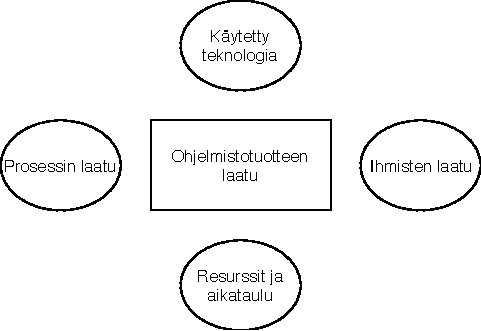
\includegraphics[scale=0.8]{images/ohjelmistonlaatu.pdf}
    \caption{Ohjelmistotuotteen latuun vaikuttavia tekijöitä \citep{sommerville}.}
    \label{fig:ohjlaatu}
\end{figure}

Suunnitelmallinen ja ketterä prosessimalli on lähestymistavaltaan ristiriidassa siinä miten prosessia tulisi kehittää. Ketterä lähestymistapa painottaa turhien hallinnollisten toimenpiteiden poistamista prosessista, korostaa siinä toimivien ihmisten osuutta laadukkaan lopputuloksen saavuttamisessa. Tarkoituksena on kehittää ihmisiä ratkaisemaan ongelmia ja oppimaan jatkuvasti uutta. Sen tavoitteena on nopea asiakkaan vaatimien toiminnallisuuksien tuottaminen ja nopea mukautuminen näiden muutoksiin.\citep{sommerville}\\

Suunnitelmallisessa lähestymistavassa kehittäminen nähdään kypsyysmallin kautta, ja se painottaa prosessijohtamisen, projektinhallinnan ja ohjelmistotuotannon hyvien käytäntöjen laajentamista organisaatiossa. Kypsyystaso kuvastaa miten laajasti ja syvällisesti hyviä käytäntöjä hyödynnetään yrityksen toiminnassa, ja kehittäminen johtaa hyvien käytäntöjen lisääntymiseen ja siten kypsyytason paranemiseen. Lähestymistavan tuloksena hallinnolliset toimenpiteet yleensä lisääntyvät suhteessa tekniseen työhön, ja tavoite on näin parantaa ohjelmistotuotteen laatua ja lisätä ennustettavuutta. \citep{sommerville}\\

Ohjelmistotuotantoon liittyvä työ on pääasiassa suunnittelutyötä, jossa korostuu luova ongelmanratkaisu \citep{kallio}. Siksi toimintamalleja voi olla vaikea kuvata ja johdon näkökulmasta on mutkikasta hallita. Liiketoimintaprosessin kehittämisen näkökulmasta tuleekin ottaa huomioon, että ohjelmiston laatu syntyy suunnittelun tuloksena, jossa yksilöiden taidoilla ja kokemuksella on suuri merkitys prosessimallista huolimatta \citep{ohjelmistotuotanto}. Toisaalta laatu saattaa kärsiä liian vähäisten resurssien, epärealistisen aikataulun tai soveltumattoman teknologian vuoksi, vaikka prosessimalli olisi sopiva ja siinä toimvat ihmiset kokeneita.\\

Ideaalia joka paikkaan sopivaa prosessimallia onkin hankala määrittää. Yleensä yrityksen käyttämä prosessi kehittyy käytännön kokemuksien kautta tunnistamalla laatuun vaikuttavat tekijät \citep{okaytannot, sommerville}. Joissain tapauksissa tarkkaan määritelty prosessi saattaa olla tärkein ohjelmiston laadun tae, kun taas joskus prosessissa toimivien ihmisten kyvyillä on suurempi vaikutus laatuun. \\

Kirjallisuudessa tuodaan esiin, että kannattavinta on usein pyrkiä mahdollisimman määrämuotoiseen prosessimallin, joka on mahdollisimman kevyt hallittavissa oleva prosessi \citep{okaytannot}. Olennaista on karsia toimintamallien monimuotoisuutta \citep{ohjelmistotuotanto, sommerville}. Tällöin prosessi ohjeistaa mitä eri vaiheissa pitäisi tehdä, vaikka suunnitelmasta joudutaankin välillä poikkeamaan. Kun toimintamallit muistuttavat projektien välillä toisiaan, on henkilöitä helpompi siirtää ja kouluttaa niiden pariin. Määrämuotoisista prosesseista on myös mahdollista kerätä hyödyllistä historiatietoja, jonka perusteella toimintaa voidaan kehittää.\\

Ohjelmistotuotantoon liittyy monia tehtäviä joiden tekeminen on aluksi suunnittelua, mutta ajan kanssa nämä tehtävät määrämuotoistuvat ja muuttuvat rutiiniksi, jotka voidaan automatisoida. Tälläisiä ovat esimerkiksi kehittämiseen käytettyjen ohjelmistojen, työkalujen ja palvelinten valitseminen ja näiden asentaminen. \citep{kallio}

Ohjelmistotuotannon automaatiolla tarkoitetaan luonnollisesti ohjelmistotuotannon toimintojen automatisoimista joko osittain tai kokonaan. Automaatio hyödyntäminen tuo ilmeisiä hyötyjä liiketoimintaprosessien kehittämisessä, mutta erityisesti ohjelmistotuotannossa hyviin käytäntöihin kuuluu rutiininomaisten ja toistuvien tehtävien automatisoiminen. \citep{leanit}

%Toimintamallien sopivuus käyttötarkoitukseen mitataan käytännössä. Projektin kohdatessa ongelmatilanteen, jos ensimmäisenä unohdetaan toimintaprosessi ja aletaan ratkomaan ongelmia kiireesti ad hoc-tavalla, on todennäköisesti aika uudistaa ohjelmistotuotannon prosessit. \citep{ohjelmistotuotanto} 

\subsection{Ohjelmistotuotanto liiketoimintaprosessissa}

Ohjelmistoja ja järjestelmiä tuottavan yrityksen liiketoimintaprosessin toimintamalleihin vaikuttaa yrityksen toimintapa ja ohjelmistotuotteen tyyppi. Ohjelmistotuotteita on kahdessa ääripäässä: Geneerisiä tuotteita, jotka ovat samanlaisia jokaiselle asiakkaalle. Räätälöityjä tuotteita, jotka tehdään täysin asiakkaan toiveiden perusteella vain sen tarpeisiin. \citep{sommerville} \\

Geneerisissä ohjelmistoissa ohjelmistoyritys kontrolloi itse vaatimuksia ja määrityksiä, kun taas räätälöidyissa ohjelmistoissa kontrolli on suurimmaksi osaksi asiakkaalla. Suurin osa ohjelmistoista tehdään räätälöidysti asiakaskohtaisissa projekteissa, mutta alalla perinteisesti pyritään hakeutumaan malliin, jossa suurin osa komponenteistä on geneerisiä \citep{sommerville}.\\

Ohjelmistoyrityksen liiketoiminnassa on kummassakin tapauksessa kolme pääprosessia: asiakasprosessi, tuotekehitysprosessi ja ylläpitoprosessi. Yrityksen ohjelmistotuote määrää liiketoimintamallin, joka vaikuttaa oleellisesti siihen miten nämä prosessit toimivat yhdessä. Asiakasprosessilla tarkoitetaan prosessia joka alkaa asiakkaan tarpeista, ja päättyy siihen kun asiakas saa ohjelmiston käyttöönsä. Tuotekehitysprosessilla tarkoitetaan niitä toimintoja, joiden avulla ohjelmistokehitystä suoritetaan. Ylläpitoprosessilla taas tarkoitetaan käyttöönoton jälkeisiä toimintamalleja. Tuotekehitys ja ylläpitoprosessi voidaan nähdä osana asiakasprosessia. \citep{okaytannot}\\

\begin{figure}[!h]
    \centering
    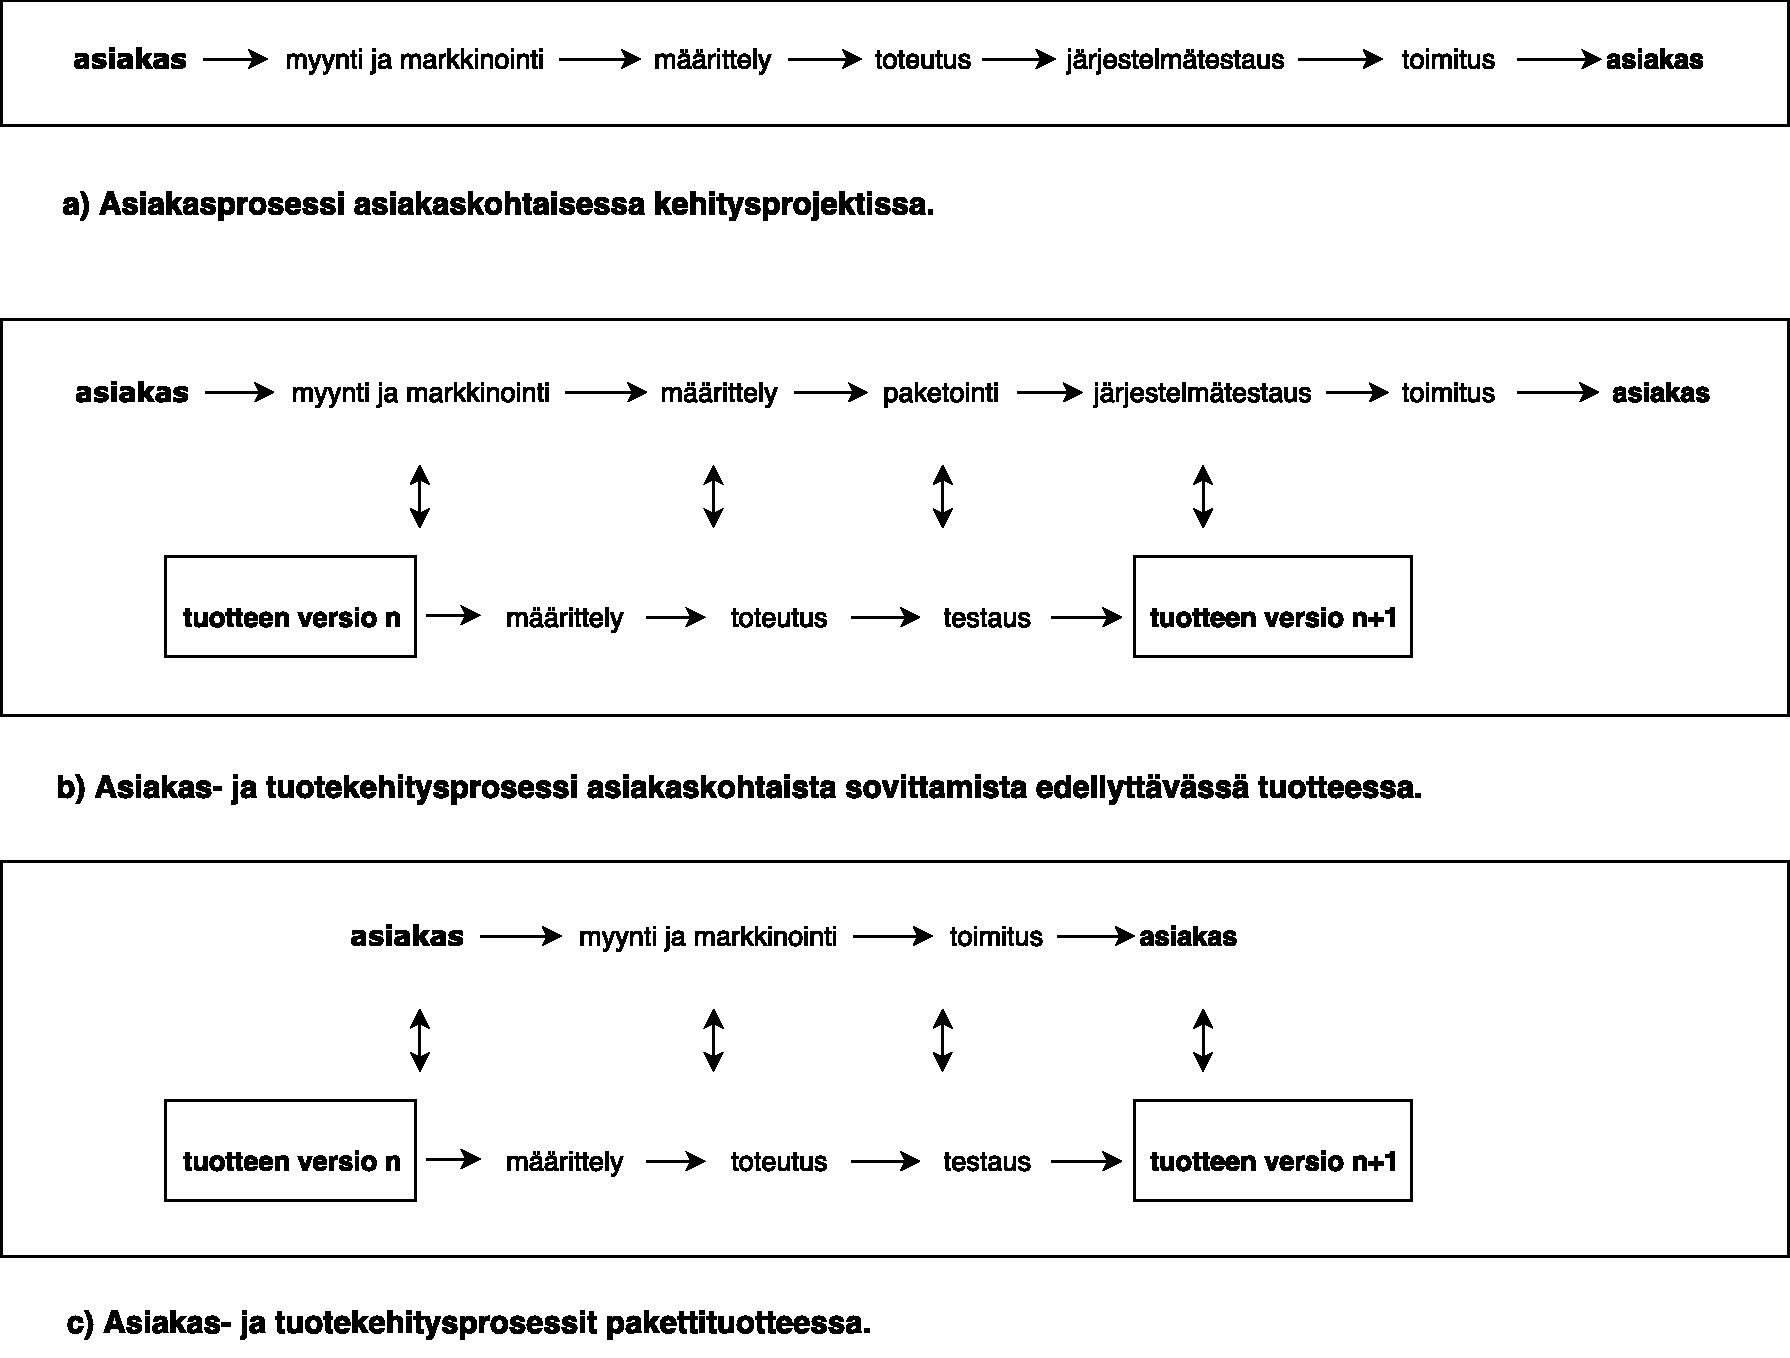
\includegraphics[scale=0.45]{asiakasprosessi.pdf}
    \caption{Asiakasprosessit eri liiketoimintamalleissa \citep{ohjelmistotuotanto}.}
    \label{fig:asiakasprosessi}
\end{figure}

Kuvassa \ref{fig:asiakasprosessi} on esimerkki asiakas- ja tuotekehitysprosessista kolmessa liiketoimintamallissa: Täysin asiakkaan tarpeiden pohjalta rakennettava ohjelmisto (a-kohta), geneerinen valmisohjelmisto (c-kohta) ja näiden ääripäiden välissä on ohjelmistoalustoihin tai ekosysteemeihin perustuva tuote (b-kohta). Kyseessä ei ole kolme eri vaihtoehtoa, vaan ohjelmistoyritykset usein mukautuvat näiden kahden ääripään välimaastoon \citep{okaytannot}.\\

Ohjelmistoyrityksen liiketoimintamalli muistuttaa yleisimmin kuvan \ref{fig:asiakasprosessi}.b-kohtaa \citep{ohjelmistotuotanto}. Tällöin tuotekehitys tuottaa perusmallin tuotteesta, joka paketoidaan asiakkaan vaatimusten mukaan. Paketoinnilla tarkoitetaan ratkaisun kokoamista olemassa olevista komponenteista esimerkiksi konfiguroimalla. Paketointi voi myös sisältää asiakaskohtaisia muutoksia tai lisäyksiä, jolloin toiminta muuttuu asiakasprojektiksi. Yleisesti toimintaa tehostaakseen yritys pyrkii luomaan tuotteen joka on samanlainen asiakkaasta riippumatta. Usein todellisuus kuitenkin on, että asiakkaiden tarpeet vaihtelevat niin paljon, ettei asiakaskohtaiselta räätälöinniltä voi välttyä. Räätälöinnin määrää on kuitenkin hallittava, että varmistetaan eri versioiden ylläpidettävyys. \citep{okaytannot}\\

Asiakaskohtaista räätälöintiä vaativissa projekteissa asiakasprosessi on monimutkaisempi verrattuna geneerisen tuotteen asiakasprosessiin. Tällöin tuotteenhallinnan tuotekehitysprosessi on osa asiakasprosessia, ja määrittelyn, toteutuksen ja testauksen toimintamallit on muodostettava projektikohtaisesti. Projektit vaativat myös resurssien, aikataulujen ja tehtävien määrittämistä, joita kaikkia on usein vaikea tuntea tarkasti etukäteen. Yrityksissä on yleensä valmiit pohjat näiden toimintamallien rakentamiseen ja historiatietoa aikaisemmista vastaavista projekteista. Tästä huolimatta lopullisten kustannusten ja aikataulun tarkka ennustaminen etukäteen on vaikeampaa kuin geneerisempien tuotteiden kohdalla. Käytännössä yllättävien suunnittelemattomien tehtävien määrä voi olla jopa neljännes projektin tehtävistä sen päätyttyä. \citep{ohjelmistotuotanto}\\

Tuotekehitysprosessissa voidaan merkittävästi vaikuttaa ohjelmiston elinkaaren kustannuksiin. Geneerisen ohjelmistotuotteen elinkaarikustannuksista suurin osa koostuu ohjelmiston kehityksestä ja testauksesta \citep{sommerville}. Asiakaskohtaisen ohjelmistotuotteen kohdalla suurimmat elinkaarikustannukset koostuvat yleensä käyttöönoton jälkeisestä ylläpidosta \citep{sommerville, ohjelmistotuotanto}. Kummassakin tapauksessa suurin kustannuksia kasvattava tekijä on perinteisesti ihmistyövoima.\citep{ohjelmistotuotanto}. \\

Elinkaarikustannuksia voidaan minimoida parhaiten tuotantoprosessin alkupäässä \citep{ohjelmistotuotanto}. Huolellisen suunnittelun ja dokumentoinnin avulla voidaan välttää turhaa työtä ja virheitä toteutusvaiheessa. Tuotantoprosessista läpi päässeen laatuvirheen aiheuttamat kustannukset kertaantuvat ylläpitovaiheessa moninkertaiseksi. Ohjelmistotuotannon laadunohjauksen keskeisimpiä tavoitteita onkin virheiden ennaltaehkäisy. Virheiden tekemiseltä ei voida kuitenkaan kokonaan välttyä, mutta virheet on pyrittävä poistamaan järjestelmästä mahdollisimman aikaisessa vaiheessa, jolloin kerrannaisvaikutuksilta vältytään. Näin minimoidaan sekä virheiden korjailun (rework) aiheuttama lisätyö kehitysprojektissa, että käyttöönoton jälkeen tapahtuva ylläpitotyö. \citep{okaytannot}

%\subsection{Automaatio ohjelmistotuotannossa}

%Ohjelmistotuotannon automaatiolla tarkoitetaan luonnollisesti ohjelmistotuotannon toimintojen automatisoimista joko osittain tai kokonaan. Automaatio hyödyntäminen tuo ilmeisiä hyötyjä liiketoimintaprosessien kehittämisessä, mutta erityisesti ohjelmistotuotannossa se hyödyntäminen nähdään välttämättömäksi.

%Kappaleen alussa puhuttiin jatkuvasta trendistä, jossa yhä kompleksisempia ja laadukkaampia ohjelmistoja halutaan ottaa yhä nopeammin käyttöön. Kirjallisuudessa tuodaan esiin, ettei tässä voida onnistua kannattavasti ilman automaation hyödyntämistä ohjelmistotuotannon prosesseissa. Siksi voidaan sanoa, että ohjelmistotuotannon hyviin käytäntöihin kuuluu rutiininomaisten ja toistuvien tehtävien automatisointi.

%Erilaisia automaatiota hyödyntäviä lähestymistapoja onkin hyödynnetty ohjelmistotuotannossa monipuolisesti jo pitkään. 
% These include requirements definition, specification, architecture, design and synthesis, implementation, modelling, testing and quality assurance, verification and validation, maintenance and evolution, configuration management, deployment, reengineering, reuse and visualisation. Automated software engineering techniques have also been used in a wide range of domains and application areas including industrial software, embedded and real-time systems, aerospace, automotive and medical systems, Web-based systems and computer games.

\subsection{Kappaleen yhteenveto}

Ohjelmistotuotanto on siis käytäntöön perustuva tieteenhaara, jossa koostetaan toimintamalleja hyvien ohjelmistojen tuottamiseen. Hyvä toimintamalli johtaa ohjelmistotuotteeseen, joka vastaa asiakkaan odotuksia sopivalla kustavustasolla ja aikataululla. Koska ohjelmistojen kirjo on valtava, on hankala muodostaa ideaalia mallia hyvän ohjelmiston tuottamiseen.\\

Ohjelmistotuotannon prosessien tuloksena syntyy ohjelmistotuote, ja sen tuottamisessa pyritään käyttämään mahdollisimman paljon valmiita elementtejä. Ohjelmstotuotannon prosesseja ovat määrittely, suunnittelu, toteutus, validointi ja ylläpito. Näitä tukevat tapauskohtaisesti tuotteen-, laadun- ja vaatimustenhallinta, sekä dokumentointiin liittyvät toimenpiteet. Näitä osa-alueita voidaan käyttää suunnitelmallisessa tai ketterässä lähestymistavassa ohjelmistotuotantoon.\\

Ohjelmistotuotteen laadun kehittämisessä tulee ottaa huomioon, että sen laatu syntyy suunnitteluvaiheessa, eikä laatua voida lisätä siihen jälkikäteen. Ketterässä lähestymistavassa pyritään minimoimaan hallinnolliset toimet laadun parantamiseksi, ja suunnitelmallisessa lähestymistavassa kehitystä toteutetaan kypsyysmalliin perustuen. Toimintaprosesseja tulisi kuitenkin määrämuotoistaa, jolloin niitä voidaan mitata, kehittää ja automatisoida. \\

Ohjelmistoyrityksen liiketoimintamalliin vaikuttaa ohjelmistotuotteen tyyppi ja yrityksen toimintatapa. Pääprosesseja ovat asiakasprosessi, tuotekehitysprosessi ja ylläpitoprosessi. Asiakaskohtaisesti räätälöidyn ohjelmistotuotteen kohdalla asiakasprosessin avulla toteutetaan asiakkaan vaatimuksia vastaava ohjelmistotuote, kun taas geneerisen tuotteen asiakasprosessissa ohjelmistotuote on jo valmiina. Yleensä suurin osa ohjelmistoyrityksistä on näiden kahden ääripään välimastossa.\\

Asiakaskohtaisissa projekteissa kustannuksien ja aikataulu arvioiminen on hankalampaa ja siten haaste ohjelmistuotannon tavoitteiden kannalta. Myös projektikohtiasesti muodosstuvat toimintamallit ovat haaste esimerkiksi automaation kannalta. Hätäilyn sijaan tulisi kuitenkin keskittyä laadukkaan ohjelmistotuotteen tekemiseen, koska virheet kostautuvat ylläpitovaiheessa moninkertaisesti.

%Automaatio ohjelmistotuotannossa tarkoittaa jonkin sen alueen osittaista tai kokonaista automatisointia, jonka seurauksena saavutetaan laadukkaampia ohjelmistoja tai prosessien tehokkuutta. Apuna käytetään erilaisia tekniikoita ja käytäntöjä, joilla itse ohjelmiston toimintaan liittyviä asioita ja prosessin vaiheita voidaan mallintaa. 

%Automaatiota on hyödynnetty ohjelmistotuotannossa monipuolisesti sen eri osa-alueisiin. Esimerkkejä soveltamis

%standartisaatio mahdollistaa uusien menetelmien käyttöönoton
%Software tools provide process support by automating some process activities and by providing information about the software that is being developed.

%Ohjelmistotuotantoon liittyy monia tehtäviä joiden tekeminen on aluksi suunnittelua, mutta ajan kanssa nämä tehtävät määrämuotoistuvat ja muuttuvat rutiiniksi, joka voidaan automatisoida. Tälläisiä ovat esimerkiksi kehittämiseen käytettyjen ohjelmistojen, työkalujen ja palvelinten valitseminen ja näiden asentaminen. 

%Automated software engineering approaches have been applied in many areas of software engineering. These include requirements definition, specification, architecture, design and synthesis, implementation, modelling, testing and quality assurance, verification and validation, maintenance and evolution, configuration management, deployment, reengineering, reuse and visualisation. Automated software engineering techniques have also been used in a wide range of domains and application areas including industrial software, embedded and real-time systems, aerospace, automotive and medical systems, Web-based systems and computer games





%Ohjelmistotuotannon automatiosointiin sisältyy käytäntöjä ja tekniikoita, jolla ohjelmistoa ja sen prosesseja voidaan mallintaa.

%Ohjelmistotuotantoon liittyy monia tehtäviä joiden tekeminen on aluksi suunnittelua, mutta ajan kanssa nämä tehtävät määrämuotoistuvat ja muuttuvat rutiiniksi, joka voidaan automatisoida. Tälläisiä ovat esimerkiksi kehittämiseen käytettyjen ohjelmistojen, työkalujen ja palvelinten valitseminen ja näiden asentaminen. 


%ohjelman rakentamiseen, ymmärtämiseen,  



%Kehittämiseen liittyy olennaisena osana kehitysympäristön työkalujen, ohjelmistojen ja palvelinten valitseminen ja näiden asentaminen. Ensimmäistä kertaa tehtäessä tämä on ilman muuta suunnittelutyötä, mutta toistuessaan voi muodostua rutiiniksi. 


%Ensimmäistä kertaa tehtäessä tämä on ilman muuta suunnittelutyötä, mutta toistuessaan voi muodostua rutiiniksi. Tietotekniikassa on se mukava puoli, että kaikki rutiinit voidaan ja pitää automatisoida, niin tämäkin.

%Kuten kappaleen alussa tuotiin esiin, ohjelmistot monimutkaistuvat ja niitä halutaan ottaa käyttöön nopeammin pienemmillä kustannuksilla. Kirjallisuudessa esitetään, että ohjelmistotuotannon prosessien kehittäminen nähdään yhtenä tapana kasvattaa ohjelmistotuotteen laatua, pienentää ohjelmistotuotannon kustannuksia tai nopeuttaa asiakasprosessin läpimenoa \citep{sommerville}.\\

%Kirjallisuuden mukaan on nähtävissä kaksi keskenään ristiriidassa olevaa näkökulmaa ohjelmistotuotannon prosessien kehittämiseen:

%\begin{enumerate}
%\setlength{\itemsep}{0pt}
%    \item Ketterä lähestymistapa, jossa ohjelmistokehitys on iteratiivista ja se painottaa turhien hallinnollisten toimenpiteiden poistamista prosessista. Sen tavoitteena nähdään olevan nopea asiakkaan vaatimien toiminnallisuuksien tuottaminen ja nopea mukautuminen näiden muutoksiin.
%    \item Prosessin kypsyysmalli, joka painottaa prosessijohtamisen, projektinhallinnan ja ohjelmistotuotannon hyvien käytäntöjen laajentamista organisaatiossa. Kypsyysmalli pohjautuu suunnitelmalliseen ohjelmistotuotannon prosessimalliin, jossa kypsyystaso kuvastaa miten laajasti ja syvällisesti hyviä käytäntöjä hyödynnetään tominnassa. Tämän lähestymistavan tuloksena hallinnolliset toimenpiteet yleensä lisääntyvät, ja tavoite onkin ohjelmistotuotteen laadun parantaminen ja ennustettavuuden lisääminen.
%\end{enumerate}

%Ehkä jottain lissää

%Käytetyllä prosessilla nähdään olevan ilmeinen vaikutus ohjelmistotuotteen laatuun, mutta toisin kuin perinteisessä laatuajattelussa, ohjelmistotuotannossa käytetyn prosessin vaikutus ohjelmiston laatuun ei ole yhtä ilmeinen. \\

%jossa tuotteen laadun ajatellaan syntyvän tuotantoprosessissa, 


%  Software quality is not influenced by its manufacturing process but by its
%design process, where people’s skills and experience are significant. In some cases,
%the process used may be the most significant determinant of product quality.
%However, for innovative applications in particular, the people involved in the process
%have more influence on quality than the process used  

%Prosessien kehittäminen sisältää prosessin mittaamisen, analyysin, mallintamisen ja muutoksen. 

%Mittaamista tulisi käyttää vastaamaan määriteltyihin kysymyksiin käytetystä ohjelmsitoprosessista. Nämä kysymykset perustuvat organisaation kehittymistavoitteisiin. 

%Kolmen tyyppisiä mittareita käytetään, jotka ovat aikamitaukset, resurssien käytön mittarit ja tapahtumamittaukset. 


%Ohjelmistotuotannon prosessien kehittämiseen pätee samat lainalaisuudet kuin minkä tahansa muun prosessin. Ensin prosesseista pitää kuoitenkin 

%Ohjelmistotuotannossa toimivan laatujärjestelmän tehtävä on siis ennaltaehkäistä inhimillisiä virheitä mahdollisimman lähellä niiden aiheuttajaa, jolloin vältytään kerrannaisvaikutuksilta. Kirjallisuudessa alleviivataan, että ohjelmistotuotannossa työprosessien laatu korostuu erityisesti sen vuoksi, koska työprosessien toiminta on suurilta osin näkymätöntä, eikä laatua voi lisätä ohjelmistoihin tai järjestelmiin jälkikäteen \citep{ohjelmistotuotanto, devops}.

%Ohjelmistotuotannon prosessien kehittämisessä vaikein tehtävä on tehdä prosessit näkyviksi ja mitattaviksi \citep{sommerville}. 

%mitä mitataan myös tärkeää, mittarin määrittäminen vaikeaa






% \citeauthor{devops} jatkaakin, että ohjelmistotuotannossa laatua mittaava ja palautekontrollin sisältävä komponentti on sisällytettävä työprosessin eri vaiheisiin. \cite{okaytannot} mukaan tehtäessä ohjelmistoja korostuukin hyvät toimintatavat, jotka on määritetty tuottamaan tavoitteen mukaista laatua. \cite{ohjelmistotuotanto} sanookin, että 



%Making a process visible requires the people involved to produce information
%about the process itself. This may slow down software production because of
%the time it takes to produce these documents.

%Measuring performance in the domain of software is hard—in
%part because, unlike manufacturing, the inventory is invisible


%Another Forrester report
%states that DevOps is accelerating technology, but that organizations
%often overestimate their progress (Klavens et al. 2017).
%Furthermore, the report points out that executives are especially
%prone to overestimating their progress when compared to those
%who are actually doing the work.



%DevOps

%The Lean IT journey
%depends on continuously improving people, process, and technology, in


%\subsection{Automaatio ohjelmistotuotannossa}

%Test automation
%COnfiguration management
%CI CD

%Ohjelmistotuotteet koostuvat useista erilaisista komponenteista ja niiden erilaisista variaatioista, jotka kehittyvät tuotteen elinkaaren aikana. Ohjelmistotuotteen versio koostuu määrätystä komponenttien kokoelmasta. Tuotteenhallinta on tukitoiminto, jossa määritellään näihin asioihin liittyvät toimintatavat ja menetelmät. \citep{okaytannot}\\

%Tuotehallinta on yksinkertaisimmillaan silloin kun ohjelmistotuotteessa olevien variaatioiden määrä on pieni. Tällöin tuotteenhallinta on pääasiassa versionhallintaa, jonka tarkoituksena on helpottaa työskentelyn koordinointia tuotekehityksen aikana. Monimutkaisimmillaan tuotteenhallinta on silloin kun tuotteen konfiguraatio vaihtelee toimintaympäristöstä riippuen ja jatkokehitettävien komponenttien määrä on suuri. Jos tuotteessa on lisäksi asiakaskohtaisia sovituksia, tuotteenhallinta monimutkaistuu entisestään. \citep{okaytannot}\\



%Projektin aikana myös määritetään resurssien, aikataulujen ja tehtävien määrittämistä, 

%joita kaikkia on usein vaikea tuntea tai huomata etukäteen. Käytännössä yllättävien suunnittelemattomien tehtävien määrä voi olla jopa neljännes projektin tehtävistä sen päätyttyä\\

%Usein ongelma on historiatiedon puute vastaavista projekteista. Historiatiedon kerääminen vaatii organisaatiossa hyvin toimivaa laatujärjestelmää ja pedanttia toimintaprosessien nuodattamista, joka on usein mahdoton saavuttaa asiakaskohtaisesti muuttuvissa prosessimalleissa. Kirjoittajat esittävät, että on paradoksaalinen tosiseikka, että kaupan saa se joka on arvioinut projektin kustannukset ja valmistumispäivän eniten alakanttiin. Vaikka asiakasprojekteihin liittyykin ennalta odottamattomia asioita, ei toimintaprosessien laadusta kannata tinkiä. \citep{ohjelmistotuotanto, okaytannot}





%Helpot kuluttajapalvleut ovat tuoneet painetta myös yrityspuolen järjestelmiin,

%https://ac.els-cdn.com/S1877050916320944/1-s2.0-S1877050916320944-main.pdf?_tid=1493c49d-303c-4339-a38a-54b5c6fca395&acdnat=1524502618_261fde6e9c10ea57d680d9fd344a1ce5
%As researchers in software engineering have been highlighting whenever possible, high quality software requires
%specific skills and the adoption of good and controlled development and operation practices. Software engineering
%has the mission to offer the right tools and methods to guide users in all activities connected to the lifecycle of
%software and services, through the usage of technologies and new paradigms, still ensuring productivity of processes
%and quality of software (performance, availability, evolvability, reliability, …). In the last years, advancements have
%led to an increasing automation of aspects such as testing, deployment, management of new software releases, and,
%at the same time, have allowed researchers and practitioners to identify new approaches for creating and operating
%software and services (think of DevOps4
% as an example). However, we cannot stop researching as the problems we
%face show increasing complexity. 



%Projektin alkuvaiheessa on vaikea tehdä rationaalisesti perusteltuja lopullisia ratkaisuja, eikä projekti voi siksi edetä alussa määritetyllä oppikirjan mukaisella prosessimallilla. Projektin alussa saadut vaatimukset muuttuvat usein projektin edetessä, ja niihin liittyvät realiteetit selviävät vasta toteutuksessa kokeilemalla. Vaikka realiteeteista olisikin hyvä käsitys alkuvaiheessa, on ihmisryhmän vaikea kollektiivisesti käsitellä niitä virheettömästi. Yksilön on helppo tarttua jo oppimaansa ratkaisuun ja siksi realiteetin vaatima toimintamalli saattaa jäädä huomaamatta. Myös jo olemassa olevien ratkaisujen uudelleenkäyttö johtaa joskus omituisiin ratkaisuihin. Näistä ongelmista huolimatta tulisi pyrkiä rationaalisen prosessimallin mahdollisimman tarkkaan seuraamiseen, koska se antaa ohjeita mitä missäkin vaiheessa pitäisi tapahtua. Tällöin projektien prosessit saadaan muistuttamaan toisiaan ja opitaan muokkaamaan niitä sopivalla tavalla tarkoituksen mukaisiksi projektin aikana, jolloin projektin suunnittelu ja seuranta on ulkopuolisenkin näkökulmasta helpompaa. Ongelmat ohjelmistotuotannossa kulminoituvat toimintaprosessin aikaisiin inhimillisiin virheisiin.\citep{ohjelmistotuotanto}

%Hyvän laatujärjestelmän yksi tavoitteista onkin estää inhimilliä erehdyksiä. Inhimillisten erehdysten estäminen raskastekoisella ja monipuolisia laatustandardeja valvovalla prosessilla ei useinkaan ole paras ratkaisu. Ohjelmistojen ja järjestelmien kanssa työskentelevillä ihmisillä on usein tapana suhtautua epäilevästi kankeisiin prosesseihin, ja sen johdosta ketterät menetelmät ovat kasvattaneet suosiotaan vastareaktiona kankealle prosessille. Hyvä työprosessi ohjelmistotuotannossa onkin mahdollisimman kevyt hallittavissa oleva prosessi. Ohjelmistotuotannossa hienoinkaan prosessi ei nimittäin korvaa tekijöiden ammattitaitoa. On kuitenkin täsmennettävä, että ohjelmistotuotannon ammattilainen tehtävään soveltuvan prosessin kanssa päihittää aina toisen ammattilaisen, jolla ei ole hyvää prosessia. Ongelmaksi muodostuu juuri sopivan prosessin rakentaminen. \citep{okaytannot}

%Ohjelmiston kehittäminen poikkeaa muista tekniikan aloista abstraktin luonteensa takia. Ohjelmistotekniikassa on myös huomattavasti vaikeampi hahmottaa rakennettavan asian koko ja monimutkaisuus. Toinen ero ohjelmistotekniikassa konkreettisiin tekniikan aloihin on tuotantotyön ja tuotantotyöläisten puuttuminen; ohjelmistojen rakentamiseen liittyvä työ on suunnittelutyötä. Ohjelmistokehityksessä pääosissa on suunnittelu, jossa formaalilla tavalla kerrotaan tietokoneelle mitä sen pitää tehdä. Ohjelmointi sekä työkalujen käyttö ja konfigurointi on suunnittelutyötä. Formaalin suunnitelman eli ohjelman muuttamisen lopulliseksi ajettavaksi järjestelmäksi hoitaa tietokone suunnittelijan formaalien ohjeiden mukaan. Kehittämiseen liittyy olennaisena osana kehitysympäristön työkalujen, ohjelmistojen ja palvelinten valitseminen ja näiden asentaminen. Ensimmäistä kertaa tehtäessä tämä on ilman muuta suunnittelutyötä, mutta toistuessaan voi muodostua rutiiniksi. Tietotekniikassa on se mukava puoli, että kaikki rutiinit voidaan ja pitää automatisoida, niin tämäkin. Ympäristö on kuitenkin standardoitu ja tärkeimmiltä osiltaan samanlainen kaikkien kehittäjien kesken. kaikki järjestelmän asennukset kaikkiin ympäristöihin että ympäristöjen asennukset tapahtuvat automaattisesti ilman manuaalisia toimenpiteitä. Kaiken pohjana on sama suunnittelutyö, joka suurimmalta osalta on tehty jo kehitysympäristön ja ensimmäisen testiympäristön synnyttyä. Oleellista on, että myös tuotantoympäristöä koskee sama automatiikka kuin muita ympäristöjä. Järjestelmän tuotantopäivitys on yhtä kevyt operaatio kuin päivitys testiympäristöön. Tuotantoprosessin automatisointi on arkipäivää ja rakennettavissa nykypäivänä yleisesti käytössä olevilla työkaluilla. Automatisoidun tuotantoprosessin suunnittelu vaatii työtä ja osa työstä on rakennettavasta järjestelmästä riippuvaista. Aivan pienessä projektissa tuotantoprosessin täydellinen automatisointi ei välttämättä maksa itseään takaisin, mutta niissäkin tärkeimmät osat pitää ehdottomasti automatisoida. \citep{kallio}

\section{Asiakaspalvelujärjestelmä ohjelmistotuotteena}
%Kappaleen tarkoitus: Kuvailla contact centereiden luonne ohjelmistotuotteena, minkälaisen ongelman ne ratkaisevat + tulevaisuuden trendejä: Integraatiot, omnichannel, CCaaS.\\
Tässä kappaleessa on tarkoitus esitellä mitä asiakaspalvelujärjestelmillä tarkoitetaan ja minkälainen ohjelmistotuote on kyseessä. Kappaleen aluksi tutustutaan hieman tähän liittyvään termistöön ja historiaan. Tämän jälkeen käydään läpi ohjelmistotuotantoon liittyviä ominaisuuksia ja tuodaan esiin tulevaisuuden trendejä.

\subsection{Asiakaspalvelujärjestelmän kuvaus}

Kirjallisuudessa asiakaspalvelujärjestelmän määritetään olevan organisaation keskitetyn yhteyskeskuksen (Contact Center) tai tutummin asiakaspalvelun resurssien käyttämä työkalu, jolla hallitaan viestintää organisaation asiakkaiden kanssa \citep{ccinfo, cisco}. Perinteisessä yhteyskeskuksessa (Call Center) viestintä keskittyy puhekanavaan, mutta nykyään asiakaspalvelujärjestelmän avulla voidaan viestiä monikanavaisesti esimerkiksi sähköpostin, pikaviestien (Instant Messaging), chattien tai sosiaalisen median kanavia käyttäen \citep{bernier, latvakoivisto}. \\

Yhteyskeskuksessa resurssit ovat tyypillisesti ihmisiä (agent) tai itsepalvelutoimintoja, jotka viestivät palvelun käyttäjien kanssa erilaisten työkalujen avulla. Viestintä palvelun käyttäjän ja palvelua tarjoavan organisaation välillä voi olla joko ulospäin (outbound) tai sisääntuleva (inbound) kontakti. Sisääntulevat kontakteissa vuorovaikutus alkaa palvelun käyttäjän toimesta ja ulospäin lähtevissä kontakteissa aloite on palvelun tarjoajalla.  \citep{ccinfo} \\

Organisaation resurssit jäsennellään erilaisten taitojen, kuten puhutun kielen tai ryhmien erikoisosaamisen perusteella\citep{cisco}. Tällöin asiakaspalvelujärjestelmän avulla voidaan yhdistää soveltuva taito tehokkaasti palvelun käyttäjien tarpeiden täyttämiseen. Tarpeiden ymmärtämiseksi hyödynnetään käytetyn kanavan tarjoamaa tietoa käyttäjästä, joka voidaan yhdistää organisaation muissa järjestelmissä olevaan asiakastietoon \citep{ccinfo}. Yhdistämisessä käytetty tieto voi perustua esimerkiksi puhevalikossa tehtyihin valintoihin, asiakkaan yhteystietoihin, käyttäjätunnuksiin tai analysoituun tietoon. Asiakaspalvelujärjestelmien avulla kerätään organisaation palvelun kannalta hyödyllistä tietoa, jonka avulla resurssien käyttöä voidaan tehostaa ja palvelua kehittää.\\

Asiakaspalvelujärjestelmät ovat monialaisia kokonaisuuksia, joiden arkkitehtuuri on monimutkaistunut merkittävästi uusien kanavien ja digitaalisten palveluiden myötä \citep{ccgartner}. Toimialalla on perinteisesti keskitytty kustannustehokkuuden optimointiin, ja mukautuminen uusiin teknologisiin innovaatioihin on hitaampaa verrattuna muihin tietotekniikan aloihin \citep{ccvarkey}. Tyypillisiä haasteita on kuvattu alla \citep{ccvissan}:

\begin{itemize}
\setlength{\itemsep}{0pt}
    \item Viestinnän kanavat toimivat siiloissa, jolloin tieto ei saatavilla muissa kanavissa tai sitä on vaikea hakea.
    \item Legacy-järjestelmien huono integroitavuus.
    \item Asiakkaan ongelmien vähäinen ymmärrys koulutuksen puutteen tai monimutkaistuvien ongelmien vuoksi.
    \item Asiakaspalvelija joutuu käyttämään useita erillisiä järjestelmiä asiakaspalvelussa. 
\end{itemize}

Tulevaisuudessa asiakaspalvelujärjestelmissä pyritään yhdistämään monikanavainen asiointi saumattomaksi (Omnichannel) asiointipoluksi. Tällöin asiakas voi viestiä organisaation kanssa haluamallaan tavalla kanavasta riippumatta ilman huolta tietokatkoksista. Myös erilaiset organisaation uudet digitaaliset palvelut yhdistyvät tietämyskantoihin, jolloin itsepalvelun määrä kasvaa. Nähdäänkin, että erilaiset tekoäly- ja robotiikkaratkaisut tulevat olennaiseksi osaksi tätä ekosysteemiä. Samalla ihmisen rooli kasvaa, koska jäljelle jäävät kontaktit ovat vaikempia ongelmia. \citep{ccgartner} \\

Asiakaspalvelujärjestelmiin liittyvät ohjelmistoprojektit ovatkin monimutkaistuneet ja muuttumassa yhä riippuvaisemmaksi organisaation yksilöllisestä toimintaympäristöstä \citep{ccinfo}. Tällöin ohjelmiston toimitusprojektiin vaikuttavien satunnaismuuttujien vaikutusta projektin ennustettavuuteen on vaikea arvioida etukäteen. Toisaalta, teknologinen kehitys esimerkiksi pilvipalvelumallin osalta on mahdollistanut kustannustehokkaiden asiakaspalvelujärjestelmien käyttöönoton pienemmissäkin organisaatioissa, ja laajentanut toimialan markkinaa \citep{ccgartner}.

\subsection{Asiakaspalvelujärjestelmä ohjelmistotuotteena}

Asiakaspalvelujärjestelmiä toteutuksessa hyödynnetään pääosin valmiita ohjelmistokomponentteja, jotka kuuluvat tiettyyn monien ohjelmistojen muodostamaan ekosysteemiin \citep{ccinfo}. Tälläiseen ekosysteemiin kuuluu erilaisia yrityksen käytössä olevia asiakashallintaan ja viestintään liittyviä järjestelmiä \citep{ccgartner}. Asiakaspalvelujärjestelmät lasketaan monissa organisaatioissa liiketoiminnan kannalta kriittisiksi järjestelmiksi, joten laatutekijöinä korostuu luotettavuus ja turvallisuus \citep{vcc}.  \\

Käytännössä organisaatiot päätyvät hyödyntämään järjestelmiä eri ohjelmistoekosysteemeistä ja nämä voivat myös olla yrityksen itsensä rakentamia legacy-järjestelmiä. Viestintään käytettyjä kanavia voi myös olla käytössä yksittäin eri siiloissa. Asiakaspalvelujärjestelmän järjestelmätoimittajan näkökulmasta suurin osa toimituksesta onkin työläiden integraatioiden läpivientiä olemassa olevien ja toimitettavan järjestelmän välillä \citep{vcc, ccinfo}. Asiakaspalvelujärjestelmissä räätälöinti tapahtuu nimenomaan integraatioilla organisaation kontekstissa oleviin järjestelmiin. Usein asiakaspalvelujärjestelmä onkin vain osa organisaatiolle toimitettavasta ratkaisusta, koska sen liiketoiminnallinen hyöty rakentuu integraatioista muihin järjestelmiin \citep{bernier}.\\

Asiakaspalvelujärjestelmän ydintoimintoja ovat kontaktien reititys ja viestintään liittyvän metriikan kerääminen \citep{vcc}. Tyypillisiä järjestelmän komponentteja ovat \citep{bernier}:

\begin{itemize}
\setlength{\itemsep}{0pt}
    \item Automaattinen puheluiden jakelu (ACD)
    \item Äänivalikko (IVR)
    \item Tietokoneen ja puhelimen integraatio (CTI)
    \item Ennustava puheluiden valinta (PD)
    \item Monitorointi-, raportointi ja analytiikkatyökalut
    \item Työpöytä ja mobiilisovellukset
\end{itemize}

Tämän lisäksi järjestelmään toiminnassa on mukana yrityksen käyttämä puhelinjärjestelmä ja puheväylä, joka liittää järjestelmän puhelinverkkoon. Asiakaspalveluärjestelmään voidaan kytkeä myös muita kanavia Internet-teknologioiden avulla ja siihen tavallisesti integroidaan organisaation sisäisiä tietojärjestelmiä. Kuvassa \ref{fig:ccarkt} on yksinkertaistettu esimerkkiarkkitehtuuri asiakaspalvelujärjestelmän kokoonpanosta. 

\begin{figure}[!h]
    \centering
    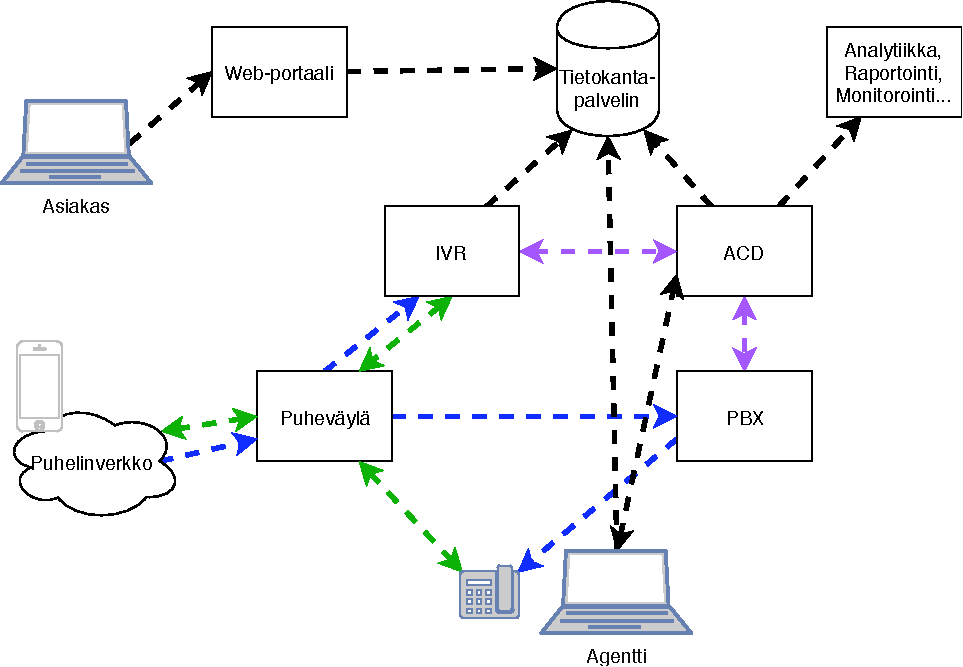
\includegraphics[scale=0.6]{images/ccarkh2.pdf}
    \caption{Asiakaspalvelujärjestelmän esimerkkiarkkitehtuuri. \citep{webrtc}}
    \label{fig:ccarkt}
\end{figure}

%Asiakaspalvelujärjestelmän sydän on automaattinen puheluiden jakaja (ACD), joka nimensä mukaisesti käsittelee saapuvia kontakteja ja jakaa ne parhaan taidon omaavalle resurssille \citep{cisco}.

Asiakaspalveluratkaisut ovat historiallisesti olleet luonteeltaan järjestelmiä, jotka on asennettu on-premises ratkaisuna yrityksen omaan konesaliin \citep{vcc}. Edelleenkin asiakaspalvelujärjestelmä saatetaan osittain asentaa on-premises ratkaisuna isojen organisaatioiden laajojen integraatio ja luotettavuus tarpeita vuoksi \citep{cisco}. Tällöin ohjelmistoprojektin kesto ja kustannukset ovat luonnollisesti korkeat. Ratkaisuissa on myös aikaisemmin korostunut laitteistokeskeskeisyys, mutta yhä useammat toimittajat pyrkivät tuottamaan tuotteistettuja valmiiksi konfiguroituja perusratkaisuja, joihin on helppo integroitua. Keskeinen ajuri on tarjota erilaisia valmiita ratkaisukokonaisuuksia niiden hankkimisen, konfiguroinnin ja toimittamisen yksinkertaistamiseksi. Tämän vuoksi ekosysteemit toimialalla ovat laajentuneet ja pilvipalvelupohjaiset Contact Center as a Service-ratkaisut nostavat suosiotaan \citep{ccinfo}. Pilvipalvelumallin tehokas hyödyntäminen contact center-ratkaisuissa on mahdollistanut sen, että yhä pienemmät yrityksen voivat ottaa ratkaisun käyttöön kustannustehokkaasti.  \\

%E, kertoo \cite{weiner}. Tällöin järjestelmä ja siihen liittyvä infrastruktuuri asennetaan yrityksen omaan konesaliin, ja yritys tai kumppani vastaa ylläpidosta. Etuna yrityksen näkökulmasta on kontrolli integroituihin järjestelmiin, niiden sisältämään dataan ja kustomointi omien tarpeiden mukaan. Selkeä haitta on isot investointikustannukset, ja rajoitetut mahdollisuudet integraatiolle ja tyypillisesti palvelutaso on heikompi kuin virtuaalisesti tuotetussa ohjelmistopalvelussa. 


 %Heidän mukaansa markkinoilla on kolmen tapaista arkkitehtuurista lähestymistapaa, yksittäisiä integroitavissa olevia täsmäratkaisuja, laajoja toimintoja tarjoavia sarjatuotteita ja palvelupohjaisia ratkaisuja. He lisäävät, että näitä ratkaisuja tarjotaan piirikytkentä perusteisena puhelinverkkoratkaisuna, IP-perusteisena ratkaisuna tai näiden kahden yhdistelminä. 

 







%Asiakaspalvelujärjestelmiä toimitetaan myös pilvipalveluna, jolloin ratkaisu tarjotaan Internetin yli ohjelmistona tai selainpohjaisena ratkaisuna päätelaitteelle. Keskeinen hyöty pilvipalvelumallissa on multitenattisuus, jolloin käyttäjät jakavat palvelun resursseja ja ovat siten kustannustehokkaita palveluntarjoajan näkökulmasta. Tämän myötä myös palvelutaso on korkea, koska kaikki on kahdennettu. Kustannukset palvelun käyttöönotossa ja käytössä ovat huomattavasti muita pienemmät. Käyttöönottoon kuluva aika on myös minimaalinen sisältäen ainoastaan tarvittavat konfiguraatiot järjestelmään. Pilvipalveluissa hyötynä on myös se, että ne integroituvat dynaamisemmin muiden selain- ja pilvipohjaisten ratkaisujen kanssa ja ne ottavat tietoturvan, yksityisyydensuojan ja palvelutason parhaiten huomioon. Selainpohjaisissa ratkaisuissa suurin haitta on se että kaikki toiminnot tapahtuvat selaimessa, jolloin sen maailman rajoitukset ovat läsnä. \citep{talkdesk}

%\cite{ccgartner} mukaan  Esimerkiksi Amazon tarjoaa tälläistä palvelua niin sanottuna Serverless-palveluna, jossa kustannus perustuu toteutuneeseen palvelun käyttöön.

%\subsection{Asiakaspalvelujärjestelmän toteutus}

%Järjestelmätoimittajien toteutumallit saattavat vaihdella paljonkin eri asiakkaiden välillä. Asiakaspalvelujärjestelmän toteutusmalli  riippuu liiketoimnnallisista vaatimuksista ja teknisen ympäristön ominaisuuksista. Seuraavassa on listattuna toteutusmalliin vaikuttavia asioita:



%Although platform redundancy, such as dual switches, voice gateways, and central con- trollers are deployed for the single-site model, the main disadvantage is the lack of a sec- ond building in a different geographic area as a backup. Without a backup system in a

%different geographic area, if the overall site suffers from power cuts or other localized issues such as a natural disaster, this could result in system downtime.



%Kuvaus lähtökohdista erilaisille asiakkaille. Koska muodostuu asiakasprojekteja ja koska on mahdollista ottaa käyttöön nopeasti.
%aspa

%Yhteydet lokaatioihin. Puhelinnumerot Asiakaspalveluratkaisu(miten monikanavainen haluaa olla, email yms. Kontaktien jako) Miten käytössä olevat työvälineet esim. crm integroituu asparatkaisuun? Ratkaisun sisällä taitojen konfigurointi (kontaktien virrat puroiksi). Raportoinnin pohjalta kehitys


%Jatkossa yrityksen luovat uusia digitaalisia palveluita asiakaskokemuksen kehittämiseksi. Tämä ennen kaikkea muuttaa tapaa jolla palveluita tuotetaan ja siten myös asiakaskohtaamiset muuttuvat. Automaattiset itsepalvelukanavat ovat contact centeriin verrattuna halvempia ylläpitää, ja contact centerin ongelmana on ollut asiakaspolun katkeilu ja siten sillä on ollut heikentävä vaikutus asiakaskokemukseen. Itsepalvelukanavien hyödyntäminen arkipäiväistyy monessa transaktiivisessa toiminnossa, ja agentti vapautuu enemmän arvoa luoviin tehtäviin. Asiakaspolun merkitys kasvaa tällöin ja siten siitä kerättävää dataa on hyödynnettävä, jotta tiedetään mitä asiakas haluaa hänen ollessa yhteydessä. Puhutaan saumattomasta asiakaskokemuksesta, jossa päästään lähemmäs intiimiä vuorovaikutusta, joka menetettiin siirrettäessä palveluita verkkoon. (deloitte)

%Seuraavassa vaiheessa asiakkaat odottavat saumatonta vuorovaikutusta palveluntarjoajilta koska tahansa ja miten tahansa.
%Asiakkaat haluavat asioida viestimällä ei soittamalla.
%Chatbotit tekevät tuloaan.
%Tekoälyn avulla tier 1 yhteydenotot vähenevät järjesstelmän älykkyys kasvaa tukitoiminnoissa.
%webrtc

\subsection{Kappaleen yhteenveto}

Asiakapalvelujärjestelmä on ohjelmistotuote, jonka avulla asiakas voi viestiä tehokkaasti organisaation kanssa. Järjestemällä tyypillisesti käsitellään useiden viestintäkanavien sisään tulevia ja ulos lähteviä kontakteja. Järjestelmän integroituu organisaation muihin tietojärjestelmiin, että resurssit voivat hyödyntää sitä viestinnässä asiakkaan kanssa.\\

Asiakaspalvelujärjestelmät ovat monialaisia kokonaisuuksia, joiden arkkitehtuuri on monimutkaistunut merkittävästi uusien kanavien ja digitaalisten palveluiden myötä. Asiakaspalvelujärjestelmiltä odotetaan jatkossa saumatonta asiakaspolkua eri kanavien välillä, ja älykkäämpää resurssien hallintaa. \\

Järjestelmät toteutetaan usein ohjelmistoprojektina, jossa kasvava monimutkaistuminen ja integrointitarpeet muodostaat kokonaisuuden jota on vaikea ennustaa etukäteen. Toisaalta pilvipohjaiset ratkaisut ovat tuoneet sen pienempien organisaatioiden saataville.\\

Asiakaspalvelujärjestelmät ovat osa organisaation viestinnän ja asiakastiedonhallinnan ekosysteemiä, jossa pyritään käyttämään valmiita ohjelmsitokomponentteja. Organisaatioissa on kuitenkin usein monimutoinen tekninen infrastruktuuri, jonka vuoksi suuri osa ratkaisun toimittamisesta on kontekstiriippuvaista integrointia.\\

Jatkossa järjestelmätoimittajat pyrkivät tuotteistamaan perusratkaisuja, jotka on yksinkertaisempi ottaa käyttöön ja helpompi integroida muihin järjestelmiin.




\section{Organisaation digitaalinen transformaatio}
%Kappaleen tarkoitus: Kuvailla miten digitaalista transformaatiota läpikäyvä yritys toimii, mitä tämä tarkoittaa operaattorin näkökulmasta ja mitkä teknologiat ovat tässä tuomassa automaatiota. Relevantti koska Telia kohdentaa uusien teknologieoiden hyödyntämisen sen keskeisimpiin liiketoimintaprosesseihin. \\\\
Monien organisaatioiden liiketoiminnan strategiassa on viime vuosina painottunut digitaalisen transformaation läpivienti \citep{lamoureux}. Tämän vuoksi tässä kappaleessa käydään läpi mitä digitaalinen transformaatio tarkoittaa ja miten se ilmenee organisaatioiden toiminnassa. Kappaleen aluksi määritellään digitaaliseen transformaatioon liittyviä termejä. Seuraavaksi esitetään kirjallisuudessa esiintynyt viitekehys, joka kuvaa organisaation toimintaa transformaation läpiviennissä. Tämän lisäksi kerrotaan miten tämä aihe liittyy erityisesti operaattorin liiketoimintaan ja strategisiin valintoihin. Lopuksi koostetaan tähän liittyviä teknologioita ja niiden käyttötapoja. Kappaleen tarkoitus on antaa kuva siitä, miten digitaalista transformaatiota läpikäyvä organisaatio toimii ja miten se vaikuttaa liiketoimintaprosesseihin.\\

\subsection{Digitaalisen transformaation määritelmä}

Kirjallisuudessa digitaalisen transformaation määritelmä on vaihdellut termin noustua esiin Internetin yleistymisen jälkeen \citep{knobel}. Viimeaikasissa määritelmissä sen ytimessä kerrotaan olevan liiketoimintamallien ja arvoketjujen uudistaminen eri aloilla sen sijaan, että kysymys olisi vain tuotteiden ja palveluiden muuttumisesta digitaalisiksi \citep{lamoureux}. Myös digitalisaation määritelmä on elänyt sen ensin kuvatessa analogisen muuttumista digitaaliseksi. Nykyään termillä kuvataan digitaalisen teknologian hyödyntämisen muutosvauhtia, jolloin käytetyt teknologiat ja toimintamallit vanhentuvat nopeammin \citep{lamoureux}. 

Yleisen paljon käytetyn määritelmän mukaan digitaalinen transformaatio on digitalisaation aiheuttamaa muutosta ihmiselämän kaikilla osa-alueilla \citep{leanit}. Koska tämä muutosvauhti kiihtyy, yritysten on omaksuttava uusi tapa kestävän liiketoiminnan rakentamiseen. Yrityksen näkökulmasta digitaalinen transformaatio määritelläänkin olevan digitaalisten teknologioiden hyödyntämistä liiketoiminnan kehittämiseen parantamalla asiakaskokemusta, liiketoimintaprosesseja ja luomalla uusia liiketoimintamalleja \citep{lamoureux}. 


The transformation stage means that digital usages inherently enable new types of innovation and creativity in a particular domain, rather than simply enhance and support traditional methods.



 A process of
information conversion from the physical to the digital plane in other words. Digital transformation 
7
however, concerns the global accelerated process of technical adaptation by individuals, businesses,
societies and nations, which comes as a result of digitalisation 


Digitaalinen transformaatio kuvaa muutosta, joka liittyy digitaalisien teknologioiden hyödyntämiseen kaikilla yhteiskunnan osa-alueilla \citep{ETSILÄHDE}. Tällöin tapahtuvaa muutosta kuvataan merkittäväksi yhteiskunnan toimintaa muuttavaksi tapahtumaksi. Muutoksen lopputuloksella ajatellaan tällöin olevan positiivinen vaikutus yhteiskunnan toimintaan, vaikka sen läpivieminen oletetaan hankalaksi ja aikaa vieväksi.

Määritelmissä myös tuodaan esiin, että transformaatio 

ajatellaan olevan yhteiskunnan toimintaa parantavia vaikutuksia.

Tapahtuva muutos on tällöin niin iso, että sen aiheuttama muutos ei kohdistu pelkästään sen toteuttajaan, vaan se muuttaa samalla myös jotain yhteiskunnan osa-aluetta.


mitä on digitaalinen, mitä on digitaalinen teknologia


The transformation stage means that digital usages inherently enable new types of innovation and creativity in a particular domain, rather than simply enhance and support traditional methods.


Digitaalisten teknologioiden hyödyntäminen yrityksen liiketoimintaprosessissa alentaa liiketominnan käyttökustannuksia ja parantaa asiakaskokemusta  \citep{lamoureux, jungner}. Lamourexin mukaan yritykset, jotka omaksuvat uusien digitaalisten teknologioiden käytön liiketoiminnassaan, suoriutuvat markkinoilla kilpailijoitaan paremmin. Hän lisää, että digitaalinen transformaatio on yrityksille selviytymisen edellytys, ja kilpailukyky markkinoilla rakentuu relevanttien teknologioiden ja niiden mahdollistamien liiketoimintavalmiuksien tunnistamiseen ja rakentamiseen. 

Digitaalisuus ja siihen liittyvä automaatio ja robotiikka ovat termeinä haastavia, koska niiden merkitys jalostuu ajan kuluessa, eri ympäristössä ja yksilöiden mielissä. Ne myös kuvaavat monimutkaisia teknologisia edistysaskelia, joita on vaikea kuvata tyhjentävästi. Keskustelussa termit myös yksinkertaistuvat ja sekoittuvat toisiinsa. Onkin tärkeä muistaa, että juuri nyt niillä tarkoitetaan asioiden tekemistä aivan uudella tavalla, eikä vain automaation tai muun uuden teknologian käyttämistä nykyisissä prosesseissa. Mooren \citeyearpar{susanmoore} mukaan kyse on uuden arvon luomisesta, eikä vain parannuksista vanhaan. Hän täsmentää, että automaatio ei vähennä ihmistyön määrää, vaan ihmistyö kohdentuu luovien ratkaisujen tekemiseen teknologian avulla. Teknologia valjastetaan luomaan yksilöllistä arvoa ihmisille \citep{jungner, susanmoore}.

Digitaalisuus itsessään ei ole mikään uusi asia. Digitaalisten teknologioiden kehitys alkoi tietokoneen keksimisestä ja yleistymisestä. Internetin myötä tietokoneet ovat yhteydessä toisiinsa ja näin tieto on tarjolla paikasta ja ajasta riippumatta. Pilviteknologioiden myötä on mahdollista käyttää lähes rajaton määrä laskentatehoa ja tallennustilaa. Tietoliikenneyhteyksien kehittymisen myötä tietoa on mahdollista siirtää paikasta toiseen yhä nopeammin. Se mitä digitaalinen tarkoittaa, muuttuu edelleen kun aikaa kuluu. Tässä työssä digitaalisilla teknologioilla tarkoitetaan nimenomaan pilvestä saatavilla olevaa laskenta- ja tallennuskapasiteettia, sekä Internet-teknologioita, joiden avulla tietokoneet ovat yhteydessä toisiinsa. Tämä digitaalisuuden aalto on hyödyllinen monilla tavoin. 

Jungnerin \citeyearpar{jungner} mukaan hyötynä digitaalisuudessa on reaalimaailman asian muuttuminen tietokoneen ymmärtämään binäärimuotoon, jolloin tietokoneen laskentatehoa ja tallennustilaa voidaan käyttää todellisen maailman ilmiöiden seuraamiseen, ymmärtämiseen ja synnyttämiseen. Tällöin voidaan rakentaa työvälineitä mallintamaan reaalimaailman ilmiöitä tietokoneen maailmaan, siirtää reaalimaailman vuorovaikutusta tietokoneiden maailmaan ja avata tietokoneille tie toimia suoraan reaalimaailmassa. Teknologian kehitys mahdollistaa uusien toimintamallien syntymisen, joiden avulla yhä monimutkaisempia reaalimaailman asioita voidaan mallintaa tietokoneelle.

\subsection{Digitaalinen visio}

Lamourex \citeyearpar{lamoureux} kertoo, että yritys voi hyödyntää digitaalisen teknologian työvälineitä kehittääkseen tuotteita ja palveluita, tehokkaampia prosesseja ja asiakaskokemusta. Hänen mukaansa digitaalinen transformaatio tarkoittaa näiden osa-alueiden jalostumista digitaalisten teknologioiden avulla. Kaikkea ei kuitenkaan ole tarkoituksenmukaista digitalisoida kerralla, vaan jalostamisen tulisi hänen mukaansa aloittaa tunnistamalla teknologiat, joilla voidaan rakentaa liiketoimintavalmiuksia tärkeimpien pullonkaulojen ratkaisemiseen. Taulukossa \ref{tab:digkys} Lamourex esittää kysymykset, joihin digitaalisen vision antaa vastauksia.

\begin{figure}[!h]
    \centering
    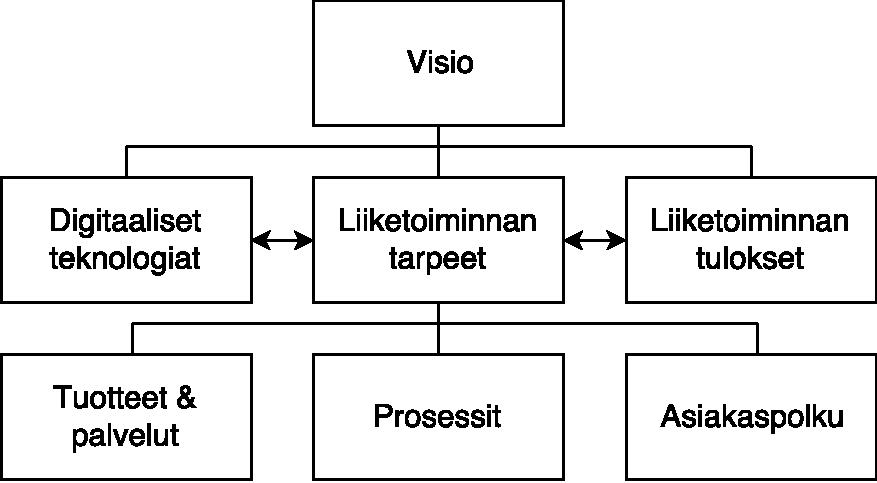
\includegraphics[scale=0.6]{images/digitaalinenvisio.pdf}
    \caption{Viitekehys digitaalisten teknologioiden hyödyntämiseen. \citep{lamoureux}}
    \label{fig:digivisio}
\end{figure}

Transformaation askeleet digitaalista visiota kohti, vaatii reaalimaailman toimintamallien arvoa tuottavan osan tunnistamista ja muuntamista tietokoneen luettavaksi, sekä arvotuotannon kehittämistä digitaalisen vision ehdoilla. Tämä vaatiikin reaalimaailmassa olevien toimintamallien pilkkomista, uudelleen järjestämistä ja eritoten karsimista \citep{leanit}. Suurin este transformaatiossa onkin organisaation vakiintunut tapa toimia, jolloin kulttuuriset näkymättömät tavat eivät sovellu digitaaliseen maailmaan \citep{jungner, lamoureux}.

MIksi transformaatio on relevantti? Sen avulla voi valjastaa digitaalisen tekemään työtä ja keskittyä luovaan asiakkaan ksilöllisseen palvelemiseen tjsp

Jungner \citeyearpar{jungner} kertoo tietokoneiden roolin korostuvan reaalimaailmassa, joka johtaa tehokkaampaan tapaan toimia. Monenlainen toiminta siirtyy tietokoneen suoritettavaksi. Tämän myötä kokonaiset toimialat uudistuvat ja myös koko yhteiskunta. Jungner käyttää esimerkkinä pankkialaa, joka käy läpi suurta muutosta, jossa palveluiden ylläpitäminen vaatii murto-osan siitä työvoimasta mitä aikaisemmin tarvittiin. Toisaalta pankkipalvelut ovat laajempia kuin aikaisemmin. Jungner alleviivaakin, että ei-digitaalisella tavalla toimiessa nykyinen pankkitoiminta vaatisi koko Suomen kansan työpanoksen. Lamourex \citeyearpar{lamoureux} korostaa, että
uusien teknologioiden hyödyntäminen ei ole vaihtoehto, vaan selviytymisen edellytys.

Jungner \citeyearpar{jungner} puhuu talouden ekosysteemin luovan tuhon kiihtymisestä nopeutuvan digitaalisuuden vuoksi, jossa vanhat yritykset, tuotteet, palvelut, tavat ja ammatit häviävät uusien tuottavampien sovellusten tieltä. Uusissa ammateissa työtavat muuttuvat hyödyntämään verkostoneituneita työvälineitä, ja tiedon hyödyntäminen tehostuu, jolloin innovaatioiden sykli nopeutuu. 

Lamourexin \citeyearpar{lamoureux} mukaan digitaalisten teknologioiden hienostuneisuus ja lukumäärä kasvaa innovaatioiden syklin nopeuduttua. Tämän myötä myös käyttötavat moninkertaistuvat. Uusien teknologioiden ja niiden käyttötapojen tehokkaalla hyödyntämisellä on mahdollista saada aikaan yhä isompia tuloksia, hän lisää. Pienet toimijat voivat vallata siivun markkinasta isommilta toimialan johtajilta tehokkaasti kohdennetulla ja ketterällä ratkaisulla. Lamourex \citeyearpar{lamoureux} puhuu disruptoinnista, jossa haastetaan vallitseva tila uudella radikaalilla tavalla, joka tuhoaa vanhaa ja luo uutta nopeasti. Hän tuo vahvasti esiin, että disruptointi ei ole vain pienten ja ketterien organisaatioiden yksinoikeus, sillä myös suuryritys voi disruptoida markkinoita. Usein suuryrityksellä onkin etulyöntiasema jos se tunnistaa nykyisten verkostojensa ja prosessiensa vahvuudet ja kykenee tekemään rohkeita kokeiluja uusien teknologioiden kanssa. 

Jungner \citeyearpar{jungner} pohtii, että puoliksi suunniteltu on digitaalisessa maailmassa tarpeeksi hyvin tehty. Hänen mukaansa käytännön kokeilut kumppaneiden ja asiakkaiden kanssa ovat nopein tapa selvittää mikä oikeasti toimii, eikä käyttää pitkää aikaa suunnitteluun. \citeauthor{devops} \citeyearpar{devops} on myös samaa mieltä: Maali liikkuu yhä nopeammin, ja siihen osuu varmemmin jos ampuu useammin ja pienemmissä erissä. Lamourex \citeyearpar{lamoureux} muistuttaa kuitenkin, että kokeiluja ohjaa digitaalinen visio uusien teknologioden tunnistaminen, joilla voi ratkaista liiketoiminnan tarpeita ja saada aikaan tuloksia. \citeauthor{gandhi} \citeyearpar{gandhi} mukaan ratkaisevaa on havaita, että digitaalinen investointi tuottaa arvoa vasta kun se on ratkaisuna tuottamassa arvoa. Kilpailussa ovat vahvoilla toimijat, jotka osaavat laittaa uudet ratkaisut työhön asiakkaiden ja muiden kumppaneiden kanssa.

\begin{table}[h!]
    \centering
    \begin{tabular}{l}
       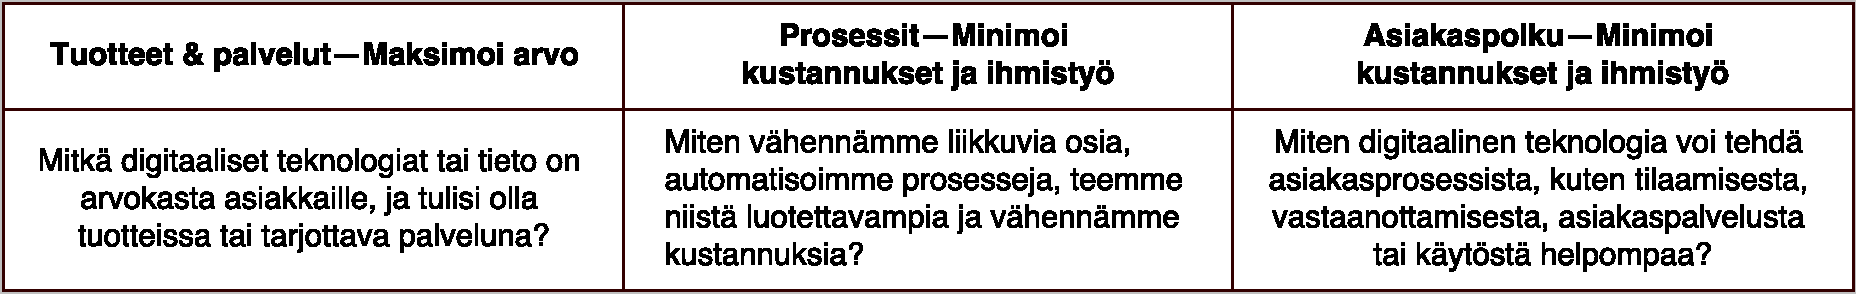
\includegraphics[scale=0.45]{images/priorisointi.pdf}
    \end{tabular}
    \caption{Kysymyksiä digitaalisen vision hahmottamiseen \citep{lamoureux}}
    \label{tab:digkys}
\end{table}

Lamourexin \citeyear{lamoureux} mukaan yrityksellä on kolme pääasiallista tapaa kehittää liiketoimintavalmiuksia markkinoilla: Kehitä tuotetta tai palvelua tekemällä siitä arvokkaampia asiakkaalle. Tehosta sisäisiä prosesseja tuottaaksesi arvo pienemmillä kustannuksilla. Paranna asiakaspolkua helpottamalla asiakkaan arvon hankkimista. Hänen mukaansa nämä osa-alueet on priorisoitava toimialan mukaan. Arvotuotannon kolme pääasiallista elementtia tuote, prosessit tai asiakaspolku korostuvat toimialan mukaan erottavana kilpailutekijänä. Investoinnit tulisi kohdentaa kilpailutekijän kehittämiseen tunnistetuille digitaalisilla teknologioilla.

Yrityksen näkökulmasta teknologialla parannetaan tuotteita, sisäisiä prosesseja ja asiakaskokemusta. Pelkästään teknologian käyttäminen ei kuitenkaan tuo hyötyä liiketoimintaan. Valitulla teknologialla täytyy olla potentiaalia kasvattaa kilpailukykyä määrätyssä aikajaksossa, ja investoinnin tulee ottaa riskit huomioon. Uusia teknologioita tulee ja menee, ja siksi tulisikin olla kykyjä tutkia useampia potentiaalisia teknologioita saman aikaisesti. Ajankohdan tulee myös olla sopiva, koska teknologiat saattavat vanhentua luultua nopeammin ja liian aikaisin tehty investointi uuteen teknologiaan saattaa heikentää kilpailuedun saamista. Teknologian hyödyntämisessä vaaditaan myös selkeä kuva liiketoimintavalmiudesta joka halutaan rakentaa sen avulla. Uusien teknologioiden käytön omaksuminen liiketoiminnan tavoitteiden saavuttamiseksi ei myöskään tapahdu itsestään. Teknologian käyttäminen kilpailuedun saavuttamiseksi markkinoilla onkin organisaation opittu taito. Eli organisaation sisäisten ja ulkoisten tavoitteen kannalta relevanttien sidosryhmien kyky tehdä yhteistyötä. Tämän kyky on vaikeampi rakentaa organisaatioissa, joissa tavoitteen kannalta relevantteja sidosryhmiä on useampia. Suurempi sidosryhmien määrä vaikeuttaa tiedon vaihtamista ja kommunikointia. Uuden teknologian hyödyntäminen kilpailiedun saavuttamiseksi vaatiikin toimintamallin muuttumista, usein yksinkertaisempaan suuntaan.

\subsection{Operaattorin digitaalinen transformaatio}

- Operaattori tekee päätöksiä ainakin osittain digitaalisen transformaation mukaan, joka ohjaa siis tekemistä. Mckinseyn raportti.\\
- Operaattoreiden haasteet muutosvoimissa

Vaikka kilpailu on ollut kovaa, perinteisesti operaattoriliiketoiminta on ollut suojassa uudelta kilpailulta, koska maantieteellistä markkinaa jakaa vain muutama operaattori. Tämä tilanne on pikkuhiljaa muuttumassa, ja operaattorit joutuvat kehittämään uusia liiketoimintamalleja vastatakseen uudenlaiseen kilpailuun. Operaattoreiden haasteet tiivistyvät kolmeen asiaan: \citep{inderes}
\begin{itemize}
    \item[] OTT-toimijat, kuten Skype ja Whatsapp, tarjoavat puhe- ja viestintäpalveluita, jotka syövät operaattoreiden tulovirtaa perinteisesti kannattavasta liiketoiminnasta.
    \item[] Kuluttajat käyttävät yhä enemmän erilaisia video- ja sosiaalisen median palveluita, ja tämän vuoksi operaattorit joutuvat investoimaan verkkokapasiteettinsa kasvattamiseen ja verkon laadun ja luotettavuuden parantamiseen. Näiden palveluiden käytöstä aiheutuu iso kuorma verkoille, mutta tuotot menevät suurelta osin OTT-toimijoille.
    \item[] Kuluttajat ja yritykset ovat yhä enemmän hintatietoisia ja vaativat parasta hinta/laatu-suhdetta verkkopalveluiltaan.
\end{itemize}

Nämä kolme asiaa heikentävät ydinliiketoiminnoista tulevaa liikevaihtoa samalla kun tarve investoinneille kasvaa. Tämän vuoksi raskas organisaatio- ja kulurakenne tuo ongelmia hintakilpailussa. Ketterät OTT-toimijat pelaavat pitkälti omilla säännöillään, kun operaattorin toimintaa rajoittaa tiukka sääntely. Perinteisesti operaattoreiden vanha IT-infrastruktuuri on myös hyvin kompleksista, joka hidastaa toimintaa. \citep{inderes}\\

Operaattori voi lähestyä tätä ongelmaa eri tavoin. Yksi strategia on keskittyä ydinliiketoimintaan ja tuottaa yhteyspalveluita mahdollisimman hyvin ja kustannustehokkaasti. Toinen strategia on vastata OTT-kilpailuun tarjoamalla omia vastaavia palveluita ja laajentua media- ja sisältö liiketoimintaan. \citep{inderes}


\subsection{Teknologiat digitaalisessa transformaatiossa}
Ns. työkalupakki jonka teknologiat tarjoavat.
Digitaalisen teknologian myötä automaatio on scriptausta apeja jne pilvessä jne. Kaikki on avointa: data, rajapinnat

Digitalisaation työkalupakki(aoit, rpa, ...)
Digitalisaation menetelmät (devops, lean, kaikki on avointa...)
Muutosvoimat operaattorin näkökulmasta(doing digital right)


Salattu liikenne? internetin päällä ei voi kulkea saalaamattomana mikään.
ihmiset tottuneet pilvipalveluiden timintaan. Voip helvetin herkkä.


teollisuudessa disruptioitiin ja sitten lähti muutos leaniin.
Automaatio ja DevOps tulee täällä. Tämän vuoksi jne.

Multi-single asiaa myös


\subsection{Kappaleen yhteenveto}

\clearpage

\section{Tutkimusmenetelmä}

Tässä kappaleessa selvennetään valittua tutkimusmenetelmää, aineiston keruumenetelmiä ja aineiston analysointia. 

\subsection{Tapaustutkimus}
Tutkimuksessa käytettiin menetelmänä tapaustutkimusta (Single Case Study). Kirjallisuudessa tapaustutkimusta kuvataan tutkimusstrategiana, jossa tarkoituksena on tutkia syvällisesti yhtä tai useampaa tapausta, ja siinä pyritään tuottamaan valitusta kohteesta yksityiskohtaista ja intensiivistä tietoa.
Lisäksi tapaustutkimuksen erityispiirteitä ovat, että siinä pyritään ymmärtämään ja tulkitsemaan yksittäistä tapausta syvällisesti sen erityisessä kontekstissa. Tälloin haetaan ilmiöön liittyvää tietoa monesta eri näkökulmasta erilaisin tavoin. \citep{jyvask} Tapaustutkimus valittiin menetelmäksi, koska tutkimuksessa haluttiin keskittyä yhden tietyn tapauksen (Kontakti L asiakasprosessin) syvälliseen ja perusteelliseen ymmärtämiseen. 

\subsection{Aineiston keruu}
Tässä tutkimuksessa aineiston keruumenetelminä käytettiin haastatteluita, löydettyä dokumentaatiota ja havainnointia. Koska kyseessä oli tapaustutkimus, jossa tutkimuskohdetta halutiinn ymmärtää syvällisesti, oli kannattavaa kerätä mahdollisimman laajasti aineistoa erilaisista aineistoista. Seuraavassa esitellään nämä kolme erilaista aineistonkeruumenetelmää ja avataan kuinka ne analysoitiin.

\subsubsection{Haastattelut}
Tutkimukseen haastateltiin 9 henkilöä, jotka haastattelujen aikaan kaikki olivat Telia Finlandin työntekijöitä. Haastateltavista kolme oli naisia ja kuusi miehiä. Yksittäisen haastatteun kesto oli noin 20-45 minuuttia. Haastatteluista kaksi suoritettiin kasvotusten, kuusi Skype viestintäkanavassa ja yksi puhelimitse. Kaikki haastattelut äänitettiin myöhempää analysointia varten. \\

Näiden haastatteluiden tarkoituksena oli saada ymmärrys Kontakti L asiakasprosessin nykytilasta. Kaikissa haastatteluissa oli mukana valmis luettelo kysymyksista eri teemojen mukaan (Liite x). Jokaisen haastattelun lähtökohtana oli käyttää puolistrukturoitua haastattelua. Puolistrukturoidussa haastattelussa kysymykset pidetään samoina kaikille haastateltaville, mutta käytössä ei ole valmiita vastausvaihtoehtoja, vaan haastateltava saa vastata kysymyksiin omin sanoin \citep{eskola}. Kuitenkin käytännössä haastatteluiden aikana yhdisteltiin puolistrukturoidun ja teemahaastattelun piirteitä. Teemahaastattelussa haastattelun teemat ovat etukäteen määrätty, mutta kysymysten tarkka muoto ja järjestys vaihtelevat \citep{eskola}. Haastatteluja käytettiin aineistonkeruumenetelmänä, koska toimintamalleista kertova dokumetaatio oli puutteellista ja haluttiin validoida jo olemassaolevaa dokumentaatiota. Haastatteluiden avulla haluttiin selvittää miten Kontakti L asiakasprosessin toimijat käytännössä suorittavat työtehtävänsä ja minkälainen käsitys heillä oli prosessin nykytilasta.\\

Haastatteluiden äänittämisen jälkeen ne litteroitiin. Litteroinnilla haastatteluiden äänitallenteet muutetaan tekstimuotoiseksi \citep{eskola}. Tässä tutkimuksessa haastatteluiden äänitetty puhe litteroitiin sanatarkasti poislukien tauot, äännähdykset ja epäselvät äänet.

\subsubsection{Löydetty dokumentaatio}\\
Haastattuiden lisäksi tutkimuksen aineistona käytettiin Telia Finlandin tuottamaa materiaalia, dokumentaatiota ja ohjeistuksia liittyen liiketoiminnan tavoitteisiin, asiakasprosessiin ja Kontakti L järjestelmään. Nämä dokumentaatiot kerättiin Telia Finlandin erilaisista tietojärjestelmistä, ja näitä olivat esimerkiksi erilaiset tekstimuotoiset ohjeistukset, videotallenteiden muistiinpanot, palaverimuistiot ja valmiit muistiinpanot.  Tutkimuksen kannalta oli oleellista käyttää vamiita olemassaolevia aineistoja ja dokumentaatioita, koska niitä oli saatavilla \citep{eskola}. Nämä dokumentaatiot valittiin tutkimusaineistoksi, koska dokumenttien tarkoituksena oli haastatteluiden ohella saada parempi kuva asiakasprosessin nykytilasta.

\subsubsection{Havainnointi}\\
Haastatteluiden ja löydetyn dokumentaation lisäksi tutkimuksen aineistona käytettiin osallistavaa havainnointia. Osallistavalla havainnoinnilla tarkoitetaan aineiston keräämistä, jossa tutkija itse osallistuu tutkimansa yhteisön toimintaan \citep{eskola}. 
Osallistava havainnointi valittiin yhdeksi aineistonkeruumenetelmäksi, koska tutkimuksen kannalta oleellista havainnointia ja tiedon keruuta oli mahdollista seurata päivittäin. 
Aineistoa kerättiin tarkkailemalla prosessissa toimivia henkilöitä ja heidän käytännön työskentelyä. Nämä kerätyt havainnot kirjoitettiin tutkijan omiksi muistiinpanoiksi ja merkinnöiksi.

\subsection{Aineiston analysointi}\\
Kerätyn aineiston analysointimenetelmänä käytettiin tyypittelyä. Tyypittelyssä aineistosta etsitään samankaltaisuuksia ja ryhmitellään ne myöhempää tarkastelua varten \citep{eskola}. Tyypittely valittiin menetelmäksi, koska tavoitteena oli luoda visuaalinen prosessikuvaus asiakasprosessista (Ks Kontakti L prosessin nykytila sivu X). Lisäksi tyypittelyn avulla saatiin kuvaus prosessissa ilmenneistä ominaisuuksista, joita oli vaikea kuvata visuaalisesti. Esimerkiksi haastateltavan näkemus asiakasprosessin haasteista (Ks. prosessissa ilmenneet haasteet sivu X). \\
\\
\\
\\




%http://dlx.b-ok.org/genesis/520000/9e7bcd4cb158cedcc21c254bb5e360c5/_as/[David_Paper,_Wai_Mok,_James_Rodger]_Building_Auto(b-ok.xyz).pdf






Kun kysyn miksi tätä prosessia ei ole automatisoitu, koostuu vastaus kahdenlaisista elementistä: Ympärillä olevat toimintamallit estävät tavoitteisiin johtavan työn tekemisen aikataulussa, jolloin ei päästä tekemään ja analysoimaan miten automaatio rakennetaan. Komponentit, jotka ovat valittavissa prosessin rakentamiseen, eivät tue automaation rakentamista halutulla tavalla, jolloin jää manuaalisia työvaiheita.

Tässä tutkimuksessa valittiin laadullinen lähestymistapa ymmärtämään/arvioimaan miksi asiakasprosessin automatisoinnissa ei ole toistaiseksi onnistuttu vertaamalla asiakasprosessin rakentamisessa käytettyjen toimintamallien ja järjestelmäkomponenttien sopivuutta suhteessa liiketoiminnan tavoitteisiin, kun tavoitteena on rakentaa automatisoitu asiakasprosessi. Arvioinnissa otetaan huomioon, että kyseessä on operaattorin contact center-liiketoiminta, ja operaattorin uudet investoinnit painottuvat digitaaliseen transformaatioon. 

Tämän lisäksi pyritään ymmärtämään syitä toimintaympäristössä liiketoimintatavoitteiden taustalla. 

Aineistopohjaisen teorian rakentaminen (grounded theory building)\\
- Menetelmässä kehitetään teoriaa ilmiöstä aineistosta löytyvien havaintojen, niiden koodauksen ja järjestämisen kautta.\\
- Teoria perustuu aineistoon, jota voidaan hankkia kenttätyössä haastatteluin ja havainnoin sekä dokumenteista.\\
- Toimii tässä tilanteessa koska nykyiset tavoitteet ovat ristiriidassa toteutuneiden asioiden kanssa, ja tilanne vaatii selvittämistä.\\
- Nykytilan havaitsemisella voidaan antaa teorian pohjalta tapoja edetä tavoitteeseen\\


\subsection{Tutkimussuunnitelma}

Single Case study: Tapaustutkimuksessa käsitellään yksittäistä, rajattua kokonaisuutta luonnollisessa ympäristössään, ja kuvaillaan tutkimuskohteen ominaispiirteitä tarkasti ja totuudenmukaisesti. Tutkittavat tapaukset ovat ainutkertaisia, ja niitä tutkitaan omassa erityisessä ympäristössään. Eli kuvataan prosessin rakentamista, jossa kolme osaa: toimija, toimintamalli tai metodi ja komponentti/työkalu.

Toiminnan nykytilan havaitseminen suhteessa tavoitteisiin:\\
- Kontakti L asiakasprosessin rakentamisen tila\\
- Kontakti M asiakasprosessin tavoitteet suhteessa toteutettuun\\
- VIP-tuotteen asiakasprosessin rakentaminen\\
- Merex-tuotteen asiakasprosessin rakentaminen\\
+ Prosessikuvaukset\\
- Miten toteutetut asiakasprosessit kehittyivät tämän jälkeen?\\
- Pasi Savilaakso, prosessivastaava (asiantuntija)\\
-> Toiminnan nykytilan havaitseminen suhteessa tavoitteisiin\\

Kontakti L-asiakasprosessiin valittavien komponenttien automatisointimahdollisuudet asiantuntijahaastatteluina\\
- Zylinc: Cloudy tiimi yritti 6 viikkoa onnistumatta\\
- Tilaus: Claudia/Salesforce, yritysportaali, Eshop (Transformaatio)\\
- Laskutus: Komarc Multibella (Transformaatio)\\
-> Valittavissa olevien komponenttien tuki automatisoinnille, ja sen mahdollistava teknologia (tarvitaanko robitiikkaa?)\\

Itsepalvelu: Asiantuntijahaastatelu\\
- Tilausvaiheen itsepalvelu\\
- Ylläpitovaiheen itsepalvelu\\

Robotiikka:\\
- Kustannus suhteessa hyötyyn: Talon sisäinen työkalu casen arviointiin kvantitatiivisena ennusteena kustannuksista ja hyödyistä. Jyrki Linsen

\subsection{Tiedon kerääminen}

Missä järjestyksessä tietoa kerätään? \\
- Käsillä olevien komponenttien analysointi\\
- Toimintamallien analysointi\\
+ muut

Puolistrukturoidut haastattelut:  Haastattelut olivat
puolistrukturoituja, jolloin kerättävä tieto oli mahdollisimman analyyttista ja
kattaa mahdollisimman laajasti aihepiirin, mutta sisältö pysyy silti aihepiirin
rajoissa.\\
+muu dokumentaatio kuten prosessikuvaukset


\subsection{Tiedon analysointi}
Haastatteluiden puhtaaksikirjoitus jokaisen haastattelun jälkeen, haastattelurunko kehittyy haastatteluiden edetessä. 


\section{Ajurit Kontakti L:n asiakasprosessin automatisoinnissa}

Tämän kappaleen tarkoituksena on kertoa mitkä ajurit ovat sen taustalla, että Kontakti L:n asiakasprosessi halutaan automatisoida. Taustalla on kaksi asiakokonaisuutta, jotka kuvataan tässä kappaleessa: Ensimmäinen on Telialla käynnissä oleva digitaalinen transformaatio, jonka myötä liiketoimintaprosesseja ja niissä käytettyjä järjestelmiä halutaan yksinkertaistaa ja automatisoida. Toinen on tyhjiö Telian yritysasiakkaille tarjoamien viestintäratkaisujen tuoteportfoliossa, jonka täyttämistä Kontakti L-tuotteella tavoitellaan. Olennaisena osana tämän tyhjiön täyttämistä on automaation hyödyntäminen Kontakti L:n asiakasprosessissa.\\

Tässä kappaleessa lähestytään näitä kahta asiakokonaisuutta Telian liiketoiminnan näkökulmasta. Ensimmäisenä käydään läpi yrityksille suunnattujen viestintäratkaisujen rooli Telian liiketoiminnassa, ja kuvataan seuraavan digitaalisen aikakauden haasteita koko yrityksen ja myös viestintäratkaisujen näkökulmasta. Tämän jälkeen kerrotaan minkälaiset strategiset tavoitteet Telia on asettanut näiden haasteiden voittamiseksi seuraavalla digitaalisella aikakaudella. Tämän avulla päästään ensimmäiseen Kontakti L:n asiakasprosessin automatisointiin vaikuttavaan asiakokonaisuuteen: Telian digitaaliseen transformaatioon, joka toteuttaa strategisia tavoitteita käytännössä.\\

Telian digitaalinen transformaatio kerrotaan kahdesta Kontakti L:n asiakasprosessiin vaikuttavasta näkökulmasta: Ensimmäisenä kuvataan miten Telian toimintamalleja pyritään uudistamaan prosessijohtamisen ja prosessiarkkitehtuuriin perustuen. Tässä kohtaa myös esitetään missä Kontakti L:n asiakasprosessi on prosessiarkkitehtuurissa. Toisena kuvataan Telian IT-järjestelmien tavoitearkkitehtuuri, johon myös Kontakti L:n asiakasprosessin järjestelmävalinnoissa tulisi pyrkiä. Tämän lisäksi kerrotaan painopisteet näissä arkkitehtuureissa, jossa digitaalista transformaatiota on lähdetty toteuttamaan.\\

Tämän kappaleen lopuksi päästään toiseen Kontakti L:n asiakasprosessin automatisointiin vaikuttavaan asiakokonaisuuteen: Tyhjiöön Telian viestintäratkaisujen tuoteportfoliossa, joka on tarkoitus täyttää Kontakti L-tuotteella. Kontakti L:n rooli tuoteportfoliossa kuvataan kahdesta näkökulmasta: Ensin esittämällä tyhjiö asiakassegmentissä, joka Kontakti L:n on tarkoitus täyttää. Toiseksi esittämällä tyhjiö alustaintegroitavuudessa, joka Kontakti L:n on tarkoitus täyttää.


%\section{Digitaalinen transformaatio Telialla}


%Tämän kappale on kuvaus Telialla käynnissä olevasta digitaalisesta transformaatiosta. Tämä on tärkeä kuvata, koska sen avulla määritetään Kontakti L:n asiakasprosessiin vaikuttavat muutosvoimat. Kappale alkaa lyhyellä esittelyllä siitä miten digitaalinen transformaatio ja asiakaspalvelujärjestelmät liittyvät Telian liiketoimintaan. Tämän jälkeen kerrotaan Telian strategisista tavoitteista seuraavalla digitaalisella aikakaudella. Lopuksi kuvataan digitaalisen transformaation muutoshanke, jonka avulla Telia pyrkii strategisiin tavoitteisiinsa. Muutoshanke kuvataan prosessiarkkitehtuurin ja IT-arkkitehtuurin näkökulmasta, jotka antavat viitekehyksen Kontakti L:n asiakasprosessin automatisointiin.

\subsection{Viestintäratkaisujen rooli Telian liiketoiminnassa}

Aikaisemmin Sonerana tunnettu Telia Finland Oyj on ruotsalaisen Telia Company-konsernin Suomen maayhtiö, jonka päätoimiala on telekommunikaation liittyvät palvelut. Yrityksen päätoimialaa on rakentaa ja ylläpitää tietoliikenteen välitystä matkapuhelin- ja lankaverkossa. Telia Finland Oyj on myös toisiksi suurin Suomessa toimiva matkapuhelinoperaattori, jonka pääkilpailijoina toimivat kotimaiset Elisa ja DNA. Kilpailua operaattoreiden välillä on kuvattu kiivaaksi viimeisten vuosien aikana \citep{hesari}. \\

Vaikka Telia onkin toisena liittymien kokonaismäärässä, on sillä ollut perinteisesti Suomessa johtava asema yritysten liittymissä \citep{hesari}. Yritysliittymien ohelle on rakentunut useita lisäpalveluita, joilla asiakas voi täydentää viestintä-, asiakaspalvelu- tai tietoliikenneratkaisuaan. Asiakaspalvelujärjestelmät, kuten Kontakti L, ovat yksi osa näitä viestintäratkaisuja. Yritysasiakkaat hakevatkin usein kokonaisvaltaista viestintäratkaisua, joka koostuu useista erilaisista tietoliikenteeseen, kommunikaatioon ja ohjelmistoihin perustuvasta komponentista. Operaattorin ydinliiketoiminnan ulkopuolisten komponenttien (kuten esimerkiksi OTT-ratkaisujen) määrä näissä viestintäratkaisuissa odotetaan kasvavan, kuten 3. kappaleessa tuotiin esiin. Vaikka operaattorin tarjoamat komponentit ovatkin välttämättömiä yritysasiakkaiden viestintäratkaisuissa, ei kokonaisratkaisua ole välttämätön hankkia Telian kaltaiselta operaattorilta. Toinen ohjelmistoyhtiö voikin tarjota paremmin asiakkaan tarvetta tai hintaodotusta vastaavan kokonaisratkaisun, jonka osana on operaattorin tarjoamat komponentit. Kuten 4. kappaleessa tuotiin esiin, erilaisten uusien digitaalisten palveluiden kasvussa on riskejä operaattorin kuten Telian liiketoiminnalle.\\

Tulevaisuuden haasteet operaattorin liiketoiminnassa on havaittu Telialla. Ketterästi ja kustannustehokkaasti uusia palveluita tuottavien ohjelmistoyhtiöiden disruptiiviseen uhkaan pyritään vastaamaan.
Tämän vuoksi Telia onkin investoinut uusiin teknologioihin, uusien palveluiden kehittämiseen ja toiminnan tehostamiseen. Tästä esimerkkinä ovat useat strategiset ohjelmistokehitykseen ja pilvipalveluihin liittyvät yritysostot, Liiga-oikeuksien hankkiminen, uuden Helsinki Data Centerin rakentaminen ja uusien digitaalisten palveluiden kehittäminen. Myös asiakaspalvelujärjestelmien osalta on tunnistettu vastaavia haasteita nykyisessä liiketoiminnassa. Näistä haasteista kerrotaan tarkemmin tämän kappaleen lopussa.\\

Voidaankin todeta, että Telian strategiana ei ole jäädä kirjallisuuskatsauksessa mainituksi "bittiputkeksi", vaan vahvistaa verkkojaan ja tuoda tämän ympärille uusia palveluita. Telian strategiassa käytetään New Generation Telco-termiä kuvaamaan sen tulevaisuuden tavoitetilaa, joka vastaa 4.2-alaluvussa esitettyihin haasteisiin.\\

Seuraavassa pureudutaan hieman Telian liiketoiminnan tavoitteisiin, joihin pyritään digitaalisen transformaation avulla.

\subsubsection{Telian liiketoiminnan tavoitteet}

Telian konsernin strategiassa \citeyearpar{telia} kuvaataan yrityksen olevan matkalla uuden ajan operaattoriksi. Maailma muuttuu digitaaliseksi ja siksi Telian täytyy pysyä mukana tässä muutoksessa, ja säilyä relevanttina asiakkailleen.  \\

Strategiassa tuodaan esiin, että tavoitetila on mahdollinen vahvistamalla liiketoiminnan ydintä ja tutkimalla mahdollisuuksia sen lähistöllä. Liiketoiminnan ytimen vahvistamiseksi kuvataan kolme painopistettä:
\begin{itemize}
    \item Luomme arvoa erinomaisten verkkoyhteyksien avulla. Turvaamme asiakkaidemme siirtymisen puheesta dataan tulevaisuuden tarpeet täyttävillä tietoliikenneyhteyksillä.
    \item Kasvatamme asiakastyytyväisyyttä lähentymällä asiakasta. Luomme saumattomia asiakaskokemuksia eri teknologioiden, palveluiden ja kanavien avulla.
    \item Varmistamme kilpailukykyiset toiminnot yksinkertaistamalla niitä ja muuttamalla legacy-järjestelmiä ketteryyden ja kustannustehokkuuden luomiseksi.
\end{itemize}

Tämän lisäksi strategiassa mainitaan, että Telialla tutkitaan mahdollisuuksia ydinliiketoiminnan lähellä, alueilla jotka vahvistavat sitä. Näistä esimerkkeinä mainitaan investoinnit M2M-teknologiaan, mediaan, turvallisuuteen, rahoituspalveluihin ja TV-palveluihin.\\

 Suomen maayhtiössä yllä mainittua strategista muutosta toimeenpannaan digitaalisen transformaation avulla, jota nimitetään Telialla transformaatiohankkeeksi. Transformaatiohankkeen tarkoituksena on luoda kilpailukykyiset tarjoamat ja toiminnot uudelle digitaaliselle aikakaudelle. Telialla tämä tarkoittaa pyrkimystä yksinkertaisempiin tuotteisiin, asiakaskanaviin, prosesseihin, ja IT-järjestelmiin. Samalla toimintamalleja halutaan muuttaa asiakaslähtöisemmäksi. Tämä pyrkimys kilpailukykyisten toimintojen yksinkertaistamiseen, eli viimeinen mainituista tavoitteista, on tämän työn taustalla. Pureudutaan seuraavaksi tarkemmin mikä Telian nykytilassa vaatii muutosta digitaalisessa transformaatiossa.

\subsection{Transformaatiohanke}

Transformaatiohankkeen avulla yhdistettiin Telialla käynnissä olleita aikaisempia muutoshankkeita, jolloin näiden hankkeiden kokonaisuuksia yhdistettiin ja näin toimet olisivat seurattavissa saman kokonaisuuden alla. Transformaatiohankkeen tavoite ja sisältö on elänyt hankkeen ajan muutoshankkeille tyypilliseen tapaan. Päätavoitteina on kuitenkin pysynyt Telian brändin vahvistaminen, tuloksiin ja arvoihin perustuva kulttuurimuutos, digitaalisen liiketoiminnan kasvattaminen, ja automatisoidun ja laadukkaan tuotantokoneiston rakentaminen digitaalisen liiketoiminnan tukemiseksi. Uudistamista vaativat osa-alueet jaetaan karkeasti kahteen osa-alueeseen: Prosessimallit ja IT-järjestelmät. Seuraavassa hieman prosessiehin liittyvästä muutospaineesta.\\

\textbf{Toimintamallin muutos}\\

Analyysit transformaatiohankkeen taustalla paljastivat ominaisuuksia Telian toimintamalleissa, jotka aiheuttavat jäykkyyttä ja turhaa komleksisuutta liiketoiminnalle. Havaittiin, että toimintoihin keskittynyt organisaatiomalli heikensi liiketoimintaprosessien toimintaa. Liiketoimintaprosessien osat toimivat siiloissa, ollen vain vastuussa välituotoksistaan. Tällöin prosessiketju katkeili matkalla, ja vastuu koko ketjun tominnasta oli määrittämättä tai henkilöitynyttä. Prosessijohtamisen malleja oli käytössä, mutta vain yksittäisissä osakokonaisuuksissa.\\

%Asiakasprosessien osalta havaittiin, order to cash prosessi on ongelmallinen\\

\begin{figure}[!h]
    \centering
    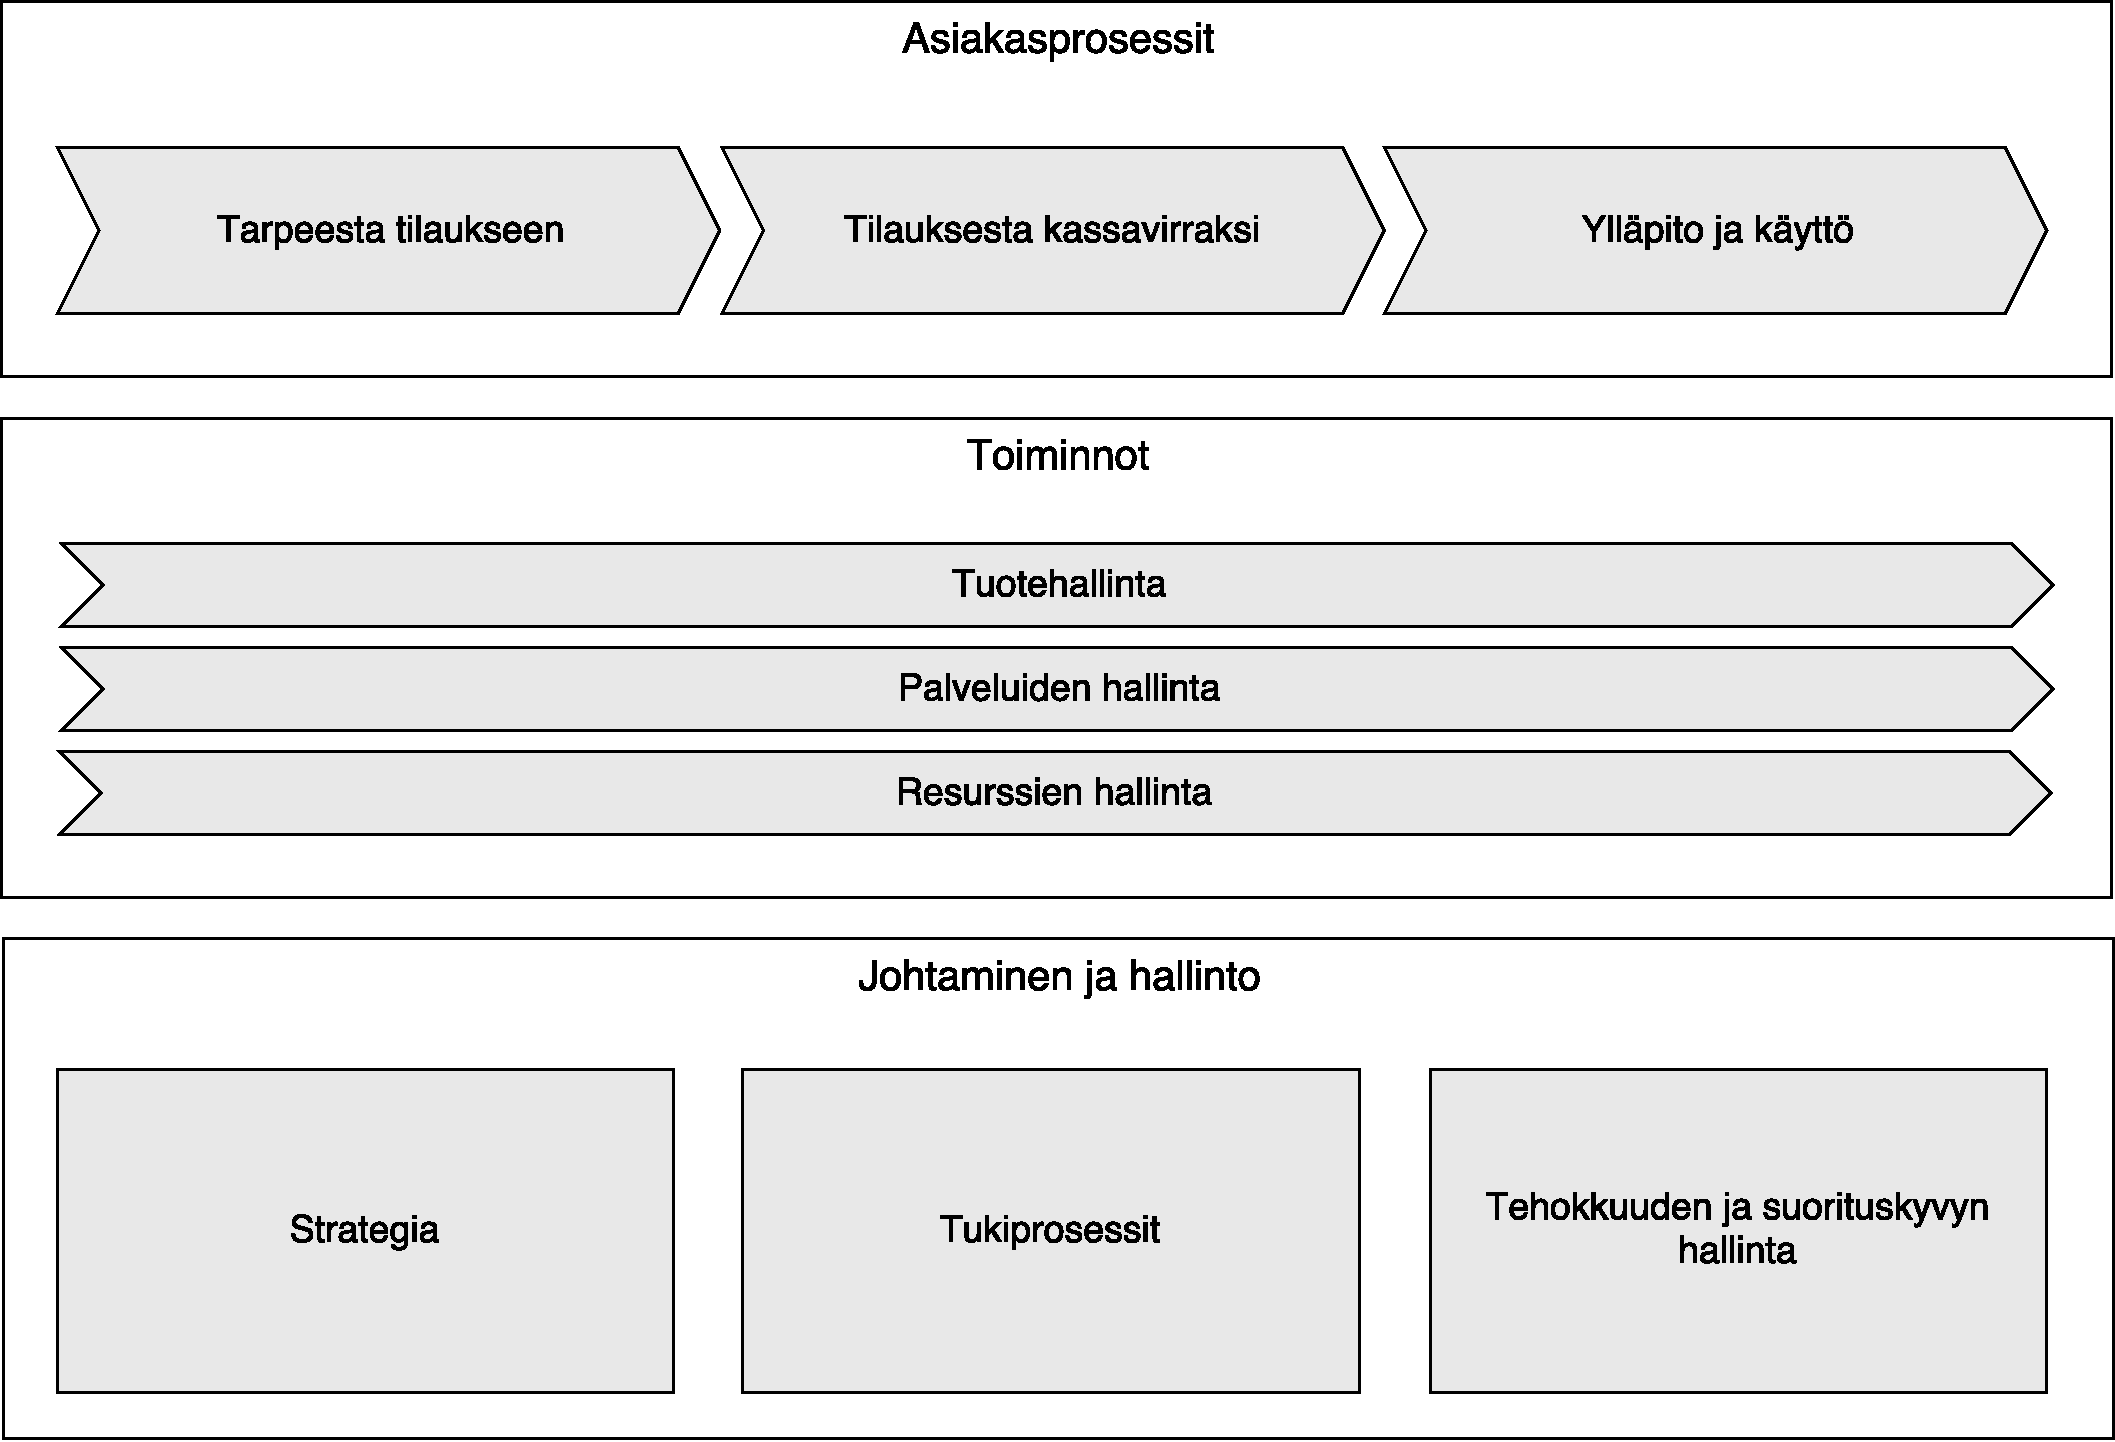
\includegraphics[scale=0.4]{images/prosessiarkkitehtuuri.pdf}
    \caption{Telian arvotuotannon prosessiarkkitehtuuri.}
    \label{fig:prosark}
\end{figure}

Siiloutunutta organisaatiomallia alettiin uusimaan prosessijohtamiseen perustuen. Segmentti ja tuotekohtaisia toimintamalleja alettiin muuttamaan perustumaan arvoketjujen ja elinkaarien johtamiseen koko liiketoiminnan kattavalla prosessimallilla. Tämän työn tuloksena määriteltiin uusi prosessiarkkitehtuuri, joka on kuvattuna kuvassa \ref{fig:prosark}. Jatkossa uusi prosessiarkkitehtuuri ja vanha toiminnallinen organisaatiomalli toimivat päällekäin, mutta toimintaa seurataan tarkemmin prosessien avulla. Kuten 2. kappaleessa kerrottiin, prosessiarkkitehtuuri kuvaa tietyn osaprosessin tehtävän, sijainnin ja tavoitteen yrityksen kokonaisarkkitehtuurissa. Se ei kuitenkaan anna vastausta siihen miten tämä käytännössä tehdään yrityksen IT-arkkitehtuurissa. Transformaatiohankeen vaikein osuus onkin juuri IT-järjestelmiin liittyvä osuus.\\

\textbf{IT-järjestelmäarkkitehtuurin muutos}\\

Analyysien mukaan kompleksisuutta tuovia ominaisuuksia on myös muissakin rakenteissa kuin organisaatiomallissa. Osin vanhasta organisaatiomallista ja vuosikymmeniä rakentuneesta IT-infrasta johtuen, IT-järjestelmien lukumäärä havaittiin korkeaksi, osin vanhanaikaiseksi, päällekäiseksi ja järjestelmät toimivat liiaksi toisista irrallaan. Toimintamallit ja käytetyt järjestelmät olivat erilaisia organisaation eri osissa. Esimerkiksi yritysasiakkaille tarjotuissa ratkaisuissa yksittäisten räätälöintien, hinnoittelumallien ja taustajärjestelmien määrän havaittiin tuovan turhaa kompleksisuutta, jota oli vaikea hallita. Laskutukseen ja asiakkuudenhallintaan käytettyjä järjestelmiä on myös useita, ja ne toimivat erillään. Jossain tapauksissa laskutus hoitui manuaalisesti Excel-työkalujen avulla. Tämän johdosta oli vaikea muodostaa kokonaisvaltaista näkymää asiakkaan ratkaisusta, ja useista erilaisista asiakkailla olevista laskutusmalleista. Myös kokonaisvaltainen näkymä asiakkailla käytössä olevista ja myytävissä olevista ratkaisuista oli vaikea muodostaa. Kokonaisuus järjestelmien osalta havaittiin kompleksiseksi ja vaikeasti hallittavaksi.\\

\begin{figure}[!h]
    \centering
    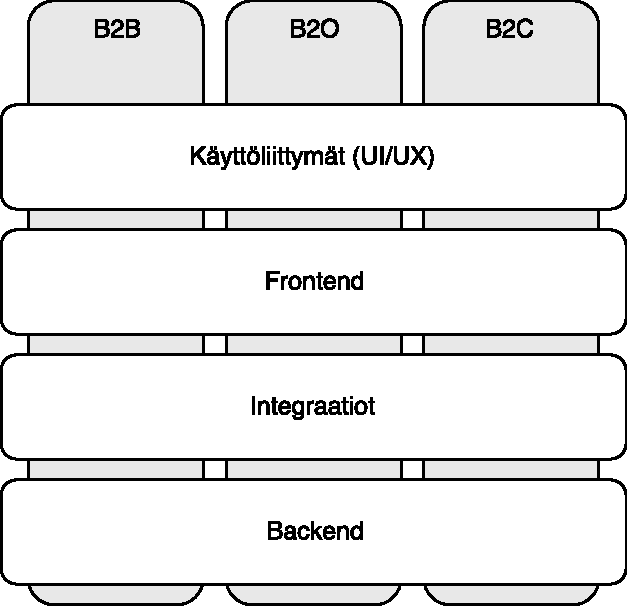
\includegraphics[scale=0.5]{images/ratkaisuarkkitehtuuri.pdf}
    \caption{Telian tavoitetilaa kuvaava IT-arkkitehtuuri.}
    \label{fig:ratkark}
\end{figure}

Transformaatiohanke lähti uudistamaan IT-järjestelmiä yllä mainittujen strategisten tavoitteiden pohjalta. Uudistustyön pohjana toimii IT-arkkitehtuurin tavoitetilan mukainen ratkaisuarkkitehtuuri, joka on esitettynä kuvassa \ref{fig:ratkark}. Tavoitearkkitehtuuri koostuu neljästä kerroksesta: Käyttöliittymä- ja frontend-kerroksista, joissa tavoitteena on parantaa asiakaskokemusta ja luoda uusia digitaalisia palveluita. Integraatio- ja backend-kerroksista, joissa tavoitteena on laskea kustannuksia ja kasvattaa laatua automaation ja migraatioiden avulla.\\

Käyttöliittymäkerros kuvaa kokoelmaa erilaisista kanavista, joista Telian asiakkaat käyttävät palveluitaan. Tämän kerroksen tarkoitus on antaa asiakkaille uusia parempia digitaalisia kanavia, joista Telian palveluita voi tilata ja hallinnoida. Aikaisemmin kuluttaja- ja yritysasiakkaille on ollut useita erilaisia järjestelmäratkaisuja ja toimintamalleja, joiden kautta palveluita hallitaan. Usein myös yksinkertaisissakin asioissa on ollut tarve kontaktoida Telian henkilöä palveluihin liittyvissä asioissa. Tämän kerroksen ratkaisujen avulla järjestelmien määrää halutaan pienentää ja suuri osa transaktioista halutaan siirtää uusiin digitaalisiin kanaviin. Tämän toivotaan parantavan asiakaskokemusta merkittävästi ja säästävän kustannuksia asiakaspalvelussa. Tämä kerros on vahvasti liitoksissa seuraavaan kerrokseen.\\

Frontend-kerros kuvaa näkymää asiakkaan palveluihin Telian henkilöille. Kuluttaja- ja yritysliiketoiminnassa ei aikaisemmin ole ollut tälläistä yhtenäistä näkymää, ja siksi sen rakentaminen koetaan tärkeäksi. Tälle kerrokselle on valittu yksi järjestelmä, joka käsittää tulevaisuudessa kaikki Telian kuluttaja- ja yritysasiakkaat. Tässä kerroksessa on myös helposti käytettävät näkymät erilaisiin asiakaspalvelutehtäviin ja myynnin työkalut. Tähän kerrokseen halutaan myös mallintaa kaikkia Telian tuotteet ja palvelut, koska tällä hetkellä tämä tieto on hajallaan erilaisissa järjestelmissä, erilaisina versioina tai se puuttuu kokonaan. Tämän kerroksen ratkaisujen avulla erilaisia tuotteita ja palveluita voidaan tuoda markkinoille nopeammin ja asiakkuuksia voidaan hallita tuloksekkaammin. Nämä kaksi ylempää kerrosta eivät kuitenkaan voi toimia ilman integraatiota taustajärjestelmiin.\\

Integraatio-kerros kuvaa sitä miten kaksi ylempää kerrosta yhdistyvät alemman backend-kerroksen tuotantojärjestelmiin. Aikaisemmin integraatioita lukuisten järjestelmien välillä rakennettiin yksittäisesti, jolloin erilaisten integraatioiden hallitseminen oli työlästä ja niiden uudelleenkäyttö ei ollut mahdollista. Jatkossa integraatio-kerros on kokoelma määriteltyjä rajapintoja, jossa on avoimia rajapintoja ja standarditeknologioita. Kerroksen avulla kumppanit ja asiakkaat voivat myös integroitua lähemmäs Telian ekosysteemiä. \\

Backend-kerros kuvaa tuotantojärjestelmiä, joissa asiakkaiden tuotteet ja palvelut toimivat, ja myös esimerkiksi laskutusjärjestelmiä. Tässä kerroksessa on vuosien mittaan rakentunut vanhojen järjestelmien kokoelma, ja myös uudet rakenteilla olevat järjestelmät. Tässä kerroksessa on myös laaja kokoelma erilaisia uusia ja vanhoja teknologioita, jonka vuoksi niiden kehittäminen on hidasta ja kallista. Tähän kerroksessa kompleksisuutta tuo myös aikaisemmin tuotelinjoitttain rakennetut tuotantojärjestelmät. Jatkossa tässä kerroksessa tavoitteena on karsia päällekkäisiä järjestelmiä ja hankkiutua eroon mahdollisimman suuresta määrästä järjestelmiä. Tämän avulla halutaan laskea kustannuksia laadukkailla ja virheettömästi toimivilla taustajärjestelmillä. Esimerkiksi tavoitteena on käyttää yhtä laskutusjärjestelmää tulevaisuudessa.\\

Transformaatiohankkeen läpivieminen nykytilasta tavoitetilaan uuden prosessiarkkitehtuurin ja IT-arkkitehtuurin avulla on iso muutos. Siksi sen läpivientiä ohjaa liiketoiminnan tavoitteet, joiden perusteella on valittu painopisteet.\\

\textbf{Transformaatiohankkeen painopisteet}\\

Transformaatiohankkeen ensimmäiksi painopisteiksi valittiin alueet, joissa oli suurin liiketoiminnallinen tarve saada tuloksia aikaan. Todettiin, että painopiste on aluksi kahdessa asiassa: Uudet tuotteet ja palvelut rakennetaan tukemaan prosessiarkkitehtuuria ja IT-arkkitehtuuria. Prosessiarkkitehtuurin ja IT-arkkitehtuurin osalta painopiste on alueissa, joissa voidaan kehittää yritysliiketoiminnan asiakaskokemusta.\\

Uusien tuotteiden ja palveluiden osalta tämä tarkoitti sitä, että niiden tulee käyttää tavoitteen mukaista IT-arkkitehtuuria. Eli näiden tuotteiden tai palveluiden tuottamiseen tulee käyttää IT-järjestelmiä, jotka toimivat myös tulevaisuuden IT-arkkitehtuurissa. Lisäksi tuotantoprosessien tulisi olla automatisoitu mahdollisuuksien rajoissa. Tämän vuoksi Kontakti L:n asiakasprosessille on myös asetettu tavoite automatisoinnista.\\

Yritysliiketoiminnan asiakaskokemuksen kehittämisessä todettiin, että tähän voitaisiin vaikuttaa eniten keskittymällä prosessiarkkitehtuurin (kuva \ref{fig:prosark}) asiakasprosesseista tarpesta tilaukseen-prosessiin. Tässä prosessissa on niiden toimintojen ketju, joiden perusteella asiakas saadaan tilaamaan tuote tai palvelu. Havaittiin, että tähän prosessiin voidaan vaikuttaa eniten kuvassa \ref{fig:ratkark} esitetyn IT-arkkitehtuurin kahdessa ylimmässä kerroksessa, jossa asiakaspolkua tukevia työkaluja voidaan rakentaa asiakkaan ja liiketoiminnan käytettäväksi.\\

Käytännön työtä on tehty pilotointien avulla rajatuissa kompakteissa toiminnoissa. Havaittiin, että toimintamallit uusissa digitaalisissa kanavissa eroavat suuresti vanhasta. Myynti, markkinointi ja asiakaspalvelu ovat erilaisia jatkossa, jonka vuoksi vasta uusien toimintamallien rakentamisen jälkeen voidaan nähdä mitä kannattaa rakentaa tai automatisoida teknologian avulla.\\

Seuraavassa alaluvussa kerrotaan Telian viestintäratkaisujen tuoteportfoliosta, joka on Telian transformaatiohankkeen lisäksi toinen Kontakti L:n automatisointia ajava asiakokonaisuus.

%Operatiivisen mallin muutos. myynti ja markkinointi asiakaspalvelu jne erilaista uusissa digitaalisissa kanavissa. iso liikeotiminnan muutos. vasta sen jälkeen tiedetään tarkemmin miten asiat kannattaa konfiguroida ja automatisoida. Sen takia liiketoiminta johtaa tätä ja sen jälkeen teknologia ja kanavat toteuttaa sen. Käyttäjälähtöistä kehitystä. 

%Tavoitetilan mukaisen prosessiarkkitehtuurin osalta todettiin, että tämä tarkoitti tarpeesta tilaukseen- asiakasprosessiin kehittämistä uusilla digitaalisilla teknologioilla. Tavoitetilan IT-arkkitehtuurin osalta tämä tarkoitti keskittymistä kahteen ylempään kerrokseen, eli käyttöliittymä- ja frontend-kerrokseen. Tarkoituksena oli siis tarjota puuttuva asiakashallinnan näkymä liiketoiminnalle, ja rakentaa asiakkaille paremmat työkalut käyttöliittymiin.\\

%Tämän jälkeen kokonaisuutta rajattiin koskemaan segmenttiä, jossa oli eniten liiketoiminnallista tarvetta parantaa asiakaskokemusta, ja missä saataisiin lyhyellä aikavälillä eniten liiketoiminnan tulosta aikaan (kuva \ref{fig:digivisio}). Eli kompakti ryhmä, jossa oli toistettavat toimintamallit ja voluumia asiakashallinnoinnissa.\\

%Ensimmäisissä piloteissa huomattiin, että uudet digitaaliset kanavat ja työkalut vaativat myös operatiivista muutosta. Olikin järkevä 

%Vanhojen toimintamallit ryhmätasolla esimerkiksi myynnissä ja markkinoinnissa eivät soveltuneet käytettäviksi uusien työkalu

%Transformaatiohankkeen painopisteet ovat olleet siellä missä lyhyellä aikavälillä voidaan saada eniten liiketoiminnallisia tuloksia aikaan, kuten 4. kappaleessa tuotiin esiin. Panopisteiksi valittiin tällä perusteella yritysliiketoiminnan keskisuuren asiakassegmentin asiakaspolun parantaminen ja uudet yrityksille lanseerattavat palvelut ja tuotteet.\\ 

%Tämä tarkoitti sitä, että prosessiarkkitehtuurin (kuva \ref{fig:prosark}) asiakasprosessin alkupää, tarpeesta tilaukseen -vaihe toimii keihäänkärkenä. IT-arkkitehtuurissa korostui sen vuoksi kaksi päällimäistä kerrosta, käyttöliittymä- ja frontend-kerros.

%Käytännössä tämä on tarkoittanut segmentin asiakkaille näkyvien asiakaskanavien käyttöliittymien uudistamisia ja segmenttiä palvelevien myyjien ja asiakaspalvelijoiden asiakasnäkymän rakentamista. 

%ei tavoittele kaikkien muutoksien läpivientiä kerralla, vaan 
%Transformaatiohankkeessa on paljon sisältöä ja tavoitteita, joten 

%otetaan käyttöön siellä missä lyhyellä aikavälillä voidaan saada eniten aikaan. Tämän vuoksi painopisteenä ovatkin olleet 
%Offer market ja sell
%asiakas se kenelle me näitä asioita teemme.
%B2B:ssä kipukohtia johon lähdettiin vaikuttamaan front endin kautta.
%Mikä on se mistä lähdetään liikkeelle?

%kaikki uudet tuotteet tuodaan target järjestelmiin. 

%Pienemmässä päässä nps haasteita ja noealla aikavälillä muutosta saada, kompaktin kokoinen ryhmä. heidän kanssa huomattavast ihelpompi harjoitella uuden homman rakentamista. Myös se että se on keskivaiheilla B2B tarjoomassa, jolloin onnistumiset voidaan hyödyntää ylhäällä ja alhaalla. 

%Mikä on se vaikein ja ensimmäinen ongelma? Asiakaskokemus se on. Puuttuvat työkalut crm ja muut liiketoiminnalle. Se mikä näkyy markkinalle. se mikä näkyy liikeotiminnalle ja antaa edellytykse t tehdä rahaa talolle.

%Operatiivisen mallin muutos. myynti ja markkinointi asiakaspalvelu jne erilaista uusissa digitaalisissa kanavissa. iso liikeotiminnan muutos. vasta sen jälkeen tiedetään tarkemmin miten asiat kannattaa konfiguroida ja automatisoida. Sen takia liiketoiminta johtaa tätä ja sen jälkeen teknologia ja kanavat toteuttaa sen. Käyttäjälähtöistä kehitystä. 

%\section{Case Kontakti L-tuotteen asiakasprosessi}

%Tässä kappaleessa käydään läpi Kontakti L:n asiakasprosessin nykytila. Nykytilan taustaksi kerrotaan Kontakti L:n liiketoimintatapaus, josta selviää asiakasprosessille asetetut vaatimukset. Tämän jälkeen käydään läpi itse asiakasprosessin nykytila kuvaamalla prosessin työvaiheet, näiden työvaiheiden kulku, prosessissa toimivat sidosryhmät ja käytetyt järjestelmät. Lopuksi kerrotaan haastatteluissa esiin nousseita haasteita asiakasprosessin nykytilassa.

\subsection{Kontakti L viestintäratkaisujen tuoteportfoliossa}

Kontakti L-tuote on uusi tuote Telian yrityksille suunnattujen viestintäratkaisujen tuoteportfoliota, jossa Kontakti L:n rooli on olla nopeasti toimitettava ja tarjota perusratkaisun lisäksi laajat integrointimahdollisuudet muihin alustoihin. Käydään seuraavassa läpi Kontakti L:n rooli tuoteportfoliossa kahdesta näkökulmasta, eli asiakassegmentin ja integroitavuuden osalta.\\

\textbf{Kontakti L:n asiakassegmentti}\\

Telian viestintäratkaisujen tuoteportfolio on jaettu asiakaspalvelujärjestelmien osalta kolmeen asiakassegmenttiin: Pieneen, keskikokoiseen ja isoon segmenttiin. Asiakassegmentit kuvastavat asiakaspalveluratkaisun toiminnallisuuden ja kompleksisuuden määrää, ei itse ratkaisua käyttävän asiakasyrityksen kokoa tai ratkaisun käyttäjämäärää. Kompleksisuudella viitataan erilaisten asiakaskohtaisten toiminnallisuuksien ja hinnoittelumallien rakentamiseen. Tuoteportfolio ja asiakassegmentit on esitetty kuvassa \ref{fig:segmentit}. Kontakti L-tuote sijoitetaan tuoteportfoliossa keskikokoiseen segmenttiin.\\

Kontakti L eroaa muista tuoteportfolion asiakaspalvelujärjestelmistä, koska se perustuu täysin Telian ulkopuolisen alihankkijan järjestelmään. Muut asiakaspalvelujärjestelmät ovat Telia-konsernin yhtiöissä kehitettyjä järjestelmiä.\\ 

\begin{figure}[!h]
    \centering
    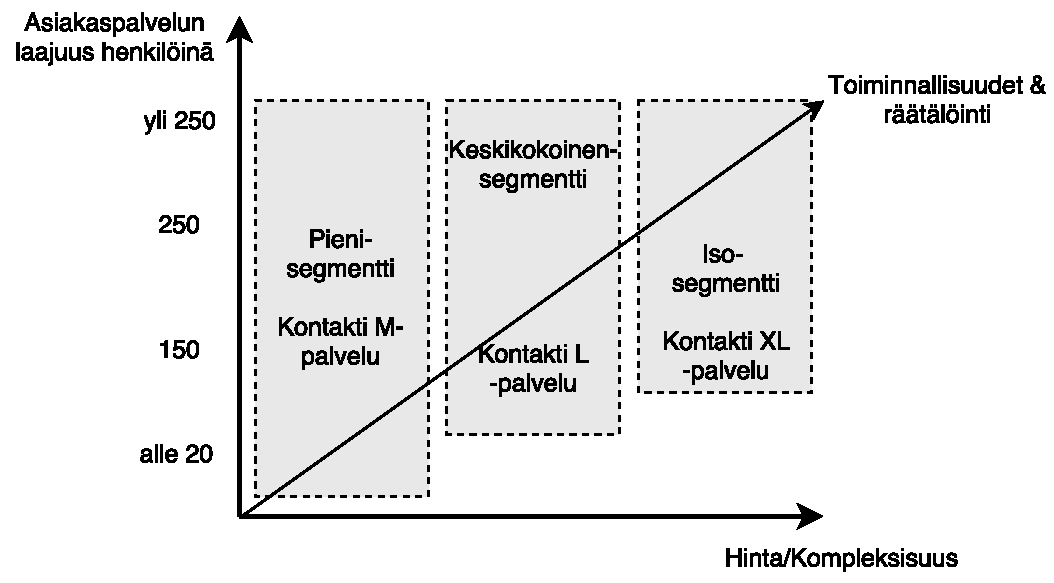
\includegraphics[scale=0.5]{images/segmentit.pdf}
    \caption{Telian asiakaspalvelujärjestelmien tuoteportfolio ja asiakassegmentit.}
    \label{fig:segmentit}
\end{figure}

Kuvan \ref{fig:segmentit} y-akseli esittää Telian asiakkaan asiakaspalvelussa työskentelevien henkilöiden lukumäärää. X-akseli taas esittää ratkaisun hintaa ja kompleksisuutta. Y- ja x-akseleiden välissä oleva nuoli kuvaa toiminnallisuuksien määrän kasvua ja myös eri räätälöintivaihtoehtojen lukumäärän kasvua. Kuvan laatikoilla esitetään miten tarpeeseen kukin ratkaisu soveltuu.\\

Asiakaspalvelujärjestelmien osalta Telia on ollut perinteinen toimija isossa segmentissä Kontakti XL-tuotteella, joka on ollut käytössä usean vuoden ajan. Sen tuottamisessa korostuu asiakaskohtaiset räätälöidyt toiminnallisuudet ja hinnoittelumallit. Myös toimitusajat ovat tällöin usein pitkiä ja ratkaisu toimitetaan asiakasprojektina. Tässä segmentissä Telia on ollut vahvin, kun taas keskikokoisessa ja pienessä segmentissä markkinaosuus on ollut heikko. Viime vuosina markkinassa onkin nähty kasvupotentiaalia nimenomaan keskikokoisessa ja pienessä segmentissä, jonka vuoksi tuoteportfoliota on täydennetty Kontakti M- ja Kontakti L-tuotteilla.\\

Pieneen asiakassegmenttiin kohdennettu Kontakti M-tuote on toiminnallisuuksilla ja räätälöintivaihtoehdoilla mitattuna yksinkertaisin ratkaisu asiakaspalveluun. Sen vahvuus on lähes automatisoitu toimitus ja asiakas voi tilata ja konfiguroida sen itse. Heikkoutena ratkaisussa on rajatut toiminnallisuudet ja integroitavuus muihin asiakkaan järjestelmiin. Tämän vuoksi Kontakti XL-tuotteen ja Kontakti M-tuotteen välille jäi tyhjiö.\\

Kontakti L-tuotteen tavoite onkin yhdistää Kontakti M- ja Kontakti XL-tuotteen parhaat puolet, eli sen tulisi olla nopeasti toimitettavissa, laskutettavissa ja tarjota perusratkaisun ohella hyvät mahdollisuudet eri alustoihin integroitumisessa, josta seuraavassa lisää.\\

\textbf{Kontakti L:n integroitavuus}\\

Kuten 3-kappaleessa tuotiin esiin, asiakaspalvelujärjestelmä integroituu yrityksen muihin järjestelmiin, kuten puheliikennettä hoitavaan järjestelmään, kalenteri- ja tilatiedon järjestelmiin sekä asiakashallinnan järjestelmiin. Markkinoilla on erilaisia alustoja joihin asiakaspalvelujärjestelmä integroituu näiden osalta, joista Telia tarjoaa pääasiassa kolmea vaihtoehtoa, jotka on esitetty kuvassa \ref{fig:palvelumal}.\\

\begin{figure}[!h]
    \centering
    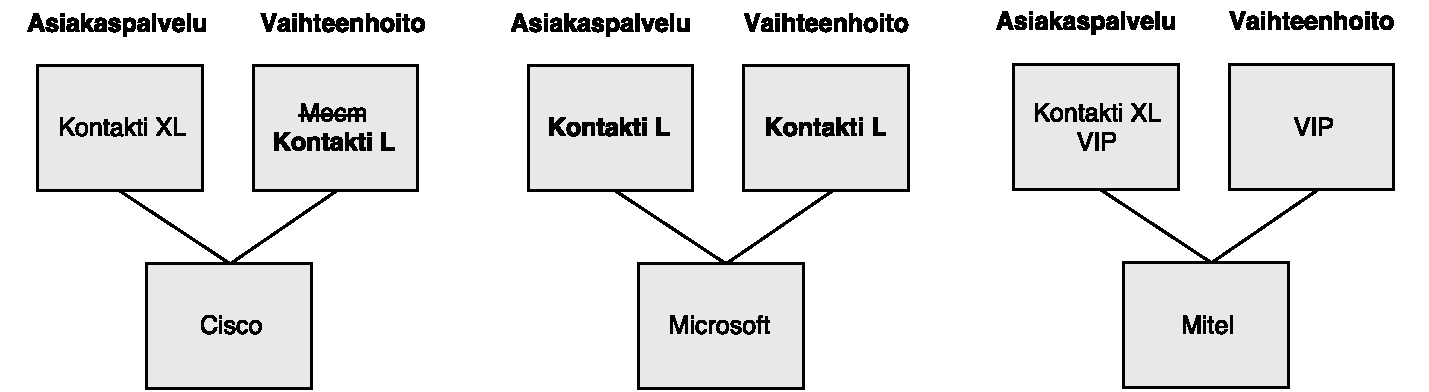
\includegraphics[scale=0.5]{images/palvelumalli.pdf}
    \caption{Telian asiakaspalveluratkaisun integroitavuus eri alustoihin.}
    \label{fig:palvelumal}
\end{figure}

%\begin{table}[]
%\centering
%\caption{My caption}
%\label{my-label}
%\begin{tabular}{|l|l|l|}
%\hline

%\textbf{Alusta:}    & \textbf{Asiakaspalvelujärjestelmä:} & \textbf{Vaihteenhoitojärjestelmä:}      \\ %\hline
%Cisco     & Kontakti XL               & Vanha: Mecm/ Uusi: Kontakti L \\ \hline
%Microsoft & Uusi: Kontakti L          & Uusi: Kontakti L              \\ \hline
%Mitel     & Kontakti XL/ VIP          & VIP                           \\ \hline
%\end{tabular}
%\end{table}

Kuvassa on esitettynä kolme eri alustaa ja kaksi erilaista ratkaisua asiakaspalvelujärjestelmän osalta. Asiakaspalvelujärjestelmä voi toimia joko perinteisenä asiakaspalvelussa käytettynä järjestelmänä tai vaihteenhoidon järjestelmänä. Kontakti L-tuotteen vahvuus onkin, että se voi toimia kumpanakin.\\

Kontakti L-tuotteella haettiin ratkaisua joka on integroitavissa Microsoftin alustan eri palveluihin. Aikaisemmin tuoteportfoliossa ei ollut ratkaisua jossa tämä onnistuisi täysin. Kontakti L-tuote myös korvaa tuoteportfoliossa elinkaarensa päässä olevan Mecm-tuotteen Ciscon ympäristössä.\\

\subsection{Kappaleen yhteenveto}

Tässä kappaleessa käytiin läpi miksi Kontakti L:n asiakasprosessi halutaan automatisoida. Automaatiota ajaa Telialla käynnissä oleva digitaalinen transformaatio ja viestintäratkaisujen tuoteportfolion tarve nopeasti toimitettavalle ratkaisulle, jossa on perusratkaisun lisäksi mahdollisuuksia integroitua muihin asiakkaan järjestelmiin.\\

Telian digitaalinen transformaatio ajaa automaatiota Kontakti L:n asiakasprosessiin, koska yksi sen painopiste on uusien tuotteiden ja palveluiden rakentaminen tavoitteen mukaiseen prosessi- ja IT-arkkitehtuuriin. Näin Kontakti L on osa kokonaisuutta joka on täyttämässä Telian strategiaa kilpailukykyisemmistä toiminnoista, joilta halutaan ketteryyttä ja kustannustehokkuutta uudella digitaalisella aikakaudella.\\

Telian viestintäratkaisujen tuoteportfoliossa asiakaspalvelujärjestelmien osalta Kontakti L:n asiakasprosessin automatisointia ajaa sen rooli keskisegmentissä, jossa yhdistyy ison ja pienen segmentin parhaat puolet. Keskisegmentin ratkaisun on oltava nopeasti toimitettavissa, mutta silti tarjota mahdollisuudet perusratkaisun lisäksi erilaisiin asiakaskohtaisiin integrointeihin. Nopeus ja asiakaskohtaiset integroinnit ovat kuitenkin ristiriidassa, ja tässä ristiriidan selvittämisessä automaatiolla on tärkeä rooli. Myös tavoitteena siirtää asiakasprosessissa tehtävää konfiguroitia asiakkaan tekemäksi itsepalveluksi.

Kontakti L:n asiakasprosessin tavoitteet vaativatkin uutta toimintamallia ja uusien teknologioiden hyödyntämistä. On tunnistettava perusratkaisu, joka voidaan automatisoida ja siirtää laskutukseen nopeasti tilauksesta, sekä tehdä vaatimuksien mukaiset integraatiot mahdolliseksi. On myös löydettävä ne toiminnot, jotka on järkevä siirtää itsepalveluun. Itsepalveluun tarvitaan myös käyttöliittymä, jonka kautta tehtävät toiminnot ovat helppoja asiakkaalle.\\

On myös ilmeistä, että näiden kahden asiakasprosessin automatisointia ajavien asiakokonaisuuksien taustalla on sama ilmiö. Uusia digitaalisia teknologioita ja ketteriä toimintamalleja hyödyntävät yritykset pystyvät luomaan uusia tehokkaampia tapoja ratkaista asiakkaan ongelma. Tällä on vaikutusta koko operaattorin liiketoimintaan ja nämä vaikutukset ovat nähtävissä myös yrityksille tarjottavien viestintäratkaisujen markkinoilla. \\

Seuraavassa kappaleessa pureudutaan Kontakti L:n asiakasprosessin nykytilaan, että voidaan arvioida sitä suhteessa sille asetettuihin tavoitteisiin.

%Kontakti L-tuote siis täydentää Telian viestintäratkaisujen tuoteportfoliota kahdella tavalla. Se tarjoaa ratkaisun asiakaspalvelujärjestelmien tuoteportfoliossa olleeseen aukkoon keskikokoisessa asiakassegmentissä, ja se tukee integraatiotioita Microsoftin alustan eri tuotteisiin.\\

%Telian kannalta markkinassa on eniten kasvupotentiaalia pienessä ja keskisuuressa asiakassegmentissä, jossa Telian markkinaosuus on pienin. Kappaleessa 4. mainittiin, että yrityksellä on kolme pääasiallista tapaa kehittää liiketoimintavalmiuksia markkinoilla: Kehitä tuotetta tai palvelua tekemällä siitä arvokkaampia asiakkaalle. Tehosta sisäisiä prosesseja tuottaaksesi arvo pienemmilläkustannuksilla. Paranna asiakaspolkua helpottamalla asiakkaan arvon hankkimista. Kuvan \ref{fig:digivisio} mukaan tavoite Kontakti L-tuotteen osalta onkin saada liiketoiminnan tuloksia aikaan tehostamalla prosesseja.

%Erityisesti Kontakti L-tuotteen osalta markkinaosuuden kasvattaminen keskisuuressa asiakassegmentissä on kiinni siitä onnistutaanko sen tuottamisessa yhdistämään Kontakti M- ja Kontakti XL-tuotteiden hyvät puolet. \\

%Asiakasprosessilta vaaditaankin nopeutta ja kustannustehokkuutta. Haaste Telian kannalta tässä onkin oikean toimintamallin löytäminen asiakasprosessissa. Kontakti L on myös uusi tuote, jonka myötä sille asetettiin uuden strategian mukaisesti tavoite korkeasta automaatioasteesta. Johdon asiakasprosessille asettama tavoite on 80-prosentin automaatio. Asiakasprosessissa tulisikin ottaa siksi huomioon sen yhteensopivuus tavoiteltuun IT-arkkitehtuuriin.
% Vendor ja IMS
%kestää pitkään että laskutus saadaan käyntiin toimituksen venyessä



%Large-segmentiin kohdennettu Kontakti XL-palvelu pohjautuu järjestelmään joka on ollut Telialla pitkään käytössä. Se on tarkoitettu asiakastarpeeseen, jolloin vaaditaan paljon erilaisia toiminnallisuuksia ja räätälöintejä, jolloin myös kustannukset ovat korkeat. Ratkaisun toimittaminen ja konfigurointi vie tällöin aikaa ja ratkaisu toimitetaan asiakaskohtaisesti projektina. Tämän kaltaisissa ratkaisuissa Telialla on iso rooli myös ylläpitovaiheessa. Tämä ratkaisu oli pitkään niin sanottu päätuote, joka integroituu Ciscon puheympäristöön ja vain osittain Microsoftin puheympäristöön. Tällöin havaittiin, että markkinassa on tarvetta hieman yksinkertaisemmalle ratkaisulle, joka on hankintakustannuksiltaan pienempi, nopeampi ottaa käyttöön, integroituisi täysin Microsoftin puheympäristöön ja soveltuisi myös pienemmän yrityksen asiakaspalveluun. Tämä tyhjiö tuoteportfoliossa jaettiin kahteen segmenttiin, low end- ja mid-segmenttiin, joihin päätettiin tuoda uudet ratkaisut.\\

 %Kyseinen ratkaisu ei integroidu muihin puheympäristöihin, vaan se käyttää omaansa. Asiakkaan kannalta ratkaisun hyötynä on nopea käyttöönotto, kustannustehokkuus ja helppo konfigurointi, jonka asiakas tekee itse. Telian kannalta ratkaisun hyötynä on lähes kokonaan automatisoitu toimitus ja asiakkaan itsepalveluna tekemä ylläpito, jonka vuoksi se ei sido resursseja ja on siten kustannuksiltaan pieni tuottaa. Kontakti M-palvelu toimii Internetin yli web-pohjaisena pilvipalveluna.\\

%Mid-segmentin osalta ratkaisu oli tuoda Kontakti L-palvelu markkinoille. Se tavoite on olla toiminnallisuuksiltaan lähes Kontakti XL:n tasoa, mutta tarjoata modernin asiakaspalvelujärjestelmän vaatimat toiminnallisuudet asiakkaille halvemmalla hinnalla, ja nopeammalla toimitusajalla. Kontakti L:n liiketoimintatapaus perustuukin halvempaan hintaan, joka on saavutettavissa tehokkaammalla toimitusprosessilla, ja integroitavuudella Microsoftin tuotteisiin ja puheympäristöön.

\section{Kontakti L:n asiakasprosessi}

Tässä kappaleessa käydään läpi Kontakti L:n asiakasprosessin nykytila. Nykytilan kuvaamiseksi kappaleessa kerrotaan ensin Kontakti L:n ratkaisuksi valitusta järjestelmästä. Tämän jälkeen esitetään yleiskuva sen asiakasprosessin nykytilasta, ja lisäksi esitetään mukana olevat sidosryhmät ja järjestelmät. Seuraavaksi kappaleessa käydään läpi asiakasprosessin eri vaiheet yksityiskohtaisesti läpi, josta ilmenee vaiheissa toimivat sidosryhmät ja järjestelmät. Lopuksi kiteytetään haastatteluissa esille nousseita haasteita asiakasprosessin eri vaiheissa.


Kuvassa \ref{fig:prosark} on kuvattuna Telian prosessiarkkitehtuuri korkealta tasolta. 


Telian prosessiarkkitehtuurin mukaan asiakasprosessi on 
Ongelmia erityisesti order-to-cash prosesseissa.
%Alt+0151

\subsection{Kontakti L:n tuotteistusprojekti}

pilotti heti isolla asiakkaalla jonka kanssa ongelmia

Tuotteistus käyntiin kiireellisellä aikataululla

Zylinc ei pystynyt toimittamaan haluttuja ominaisuuksia tuotteeseen, homma perustui multitentant juttuihin

Kaksi isoa asiakaskeissiä, jonka vuoksi tuotteistuskeskeytettiin ja keskityttiin asiakastoimituksiin.

\subsection{Kontakti L:n asiakasprosessin nykytila}

Telian prosessiarkkitehtuuri (kuva \ref{fig:prosark}) määritteli kolme erilaista asiakasprosessia: Tarpeesta tilaukseen, tilauksesta kassavirraksi ja ylläpidon ja käytön. Tämän työn tarkastelussa on 2. kappaleessa esitetty asiakasprosessi, joka on prosessiarkkitehtuurin tilauksesta kassavirraksi —asiakasprosessi. Tilauksesta kassavirraksi —asiakasprosessi luo toimintamallit tuotteen tilaamiseen, toimittamiseen ja laskuttamiseen. Telian IT-arkkitehtuurin (kuvassa \ref{fig:ratkark}) näkökulmasta prosessissa painottuu backend-kerros, jossa sijaitsee tuotanto- ja laskutusjärjestelmät.\\

Kuten edellisessä kappaleessa tuotiin esiin, Telian digitaalisen transformaation painopiste on prosessiarkkitehtuurin tarpeesta tilaukseen asiakasprosessissa ja siten IT-arkkitehtuurin kahdessa ylimmässä kerroksessa. Tästä huolimatta, koska Kontakti L on uusi tuote, on sen tilauksesta kassavirraksi asiakasprosessille annettu tavoitteeksi 80\% automaatioaste käyttämällä IT-arkkitehtuurin tavoitejärjestelmiä.\\

Telian laatujärjestelmä määrittää asiakasprosesseille niiden kehitystä kuvaavan valmiusasteen. Kontakti L:n asiakasprosessi on tämän työn kirjoittamisen hetkellä hyväksytty valmiina myyntiin —kypsyysasteelle. Tässä vaiheessa on selvillä tuotteen hinnasto ja yksityiskohdat. Asiakasprosessin toimintamallit eivät ole tässä vaiheessa vielä täysin valmiina, mutta toimituksia voidaan tehdä poikkeustapauksessa. Kontakti L ei ole vielä saanut hyväksyntää seuraavalle asteelle, joka on valmiina toimitukseen—aste. Tässä vaiheessa tuote tai palvelu on valmiina toimitettavaksi tilauksen perusteella ja kaikki asiakasprosessin toimintamallit ovat selvillä.\\

Kontakti L:n asiakasprosessin nykytila onkin on selvitetty lähes valmiiden toimintamallien ja ohjeistuksien perusteella jotka ovat muodostuneet kahden ison asiakasprojektin aikana, sekä prosessissa toimivien sidosryhmien haastatteluiden perusteella.

\subsubsection{Yleiskuva ja sidosryhmät}

Kuvassa \ref{fig:paavaih} on kuvattuna Kontakti L:n asiakasprosessin päävaiheet, toimitusprojektin osuus ja tuotekehitys asiakasprosessin osana. Käydään seuraavaksi asiakasprosessin päävaiheet ja toimijat läpi yleisellä tasolla.\\

\begin{figure}[!h]
    \centering
    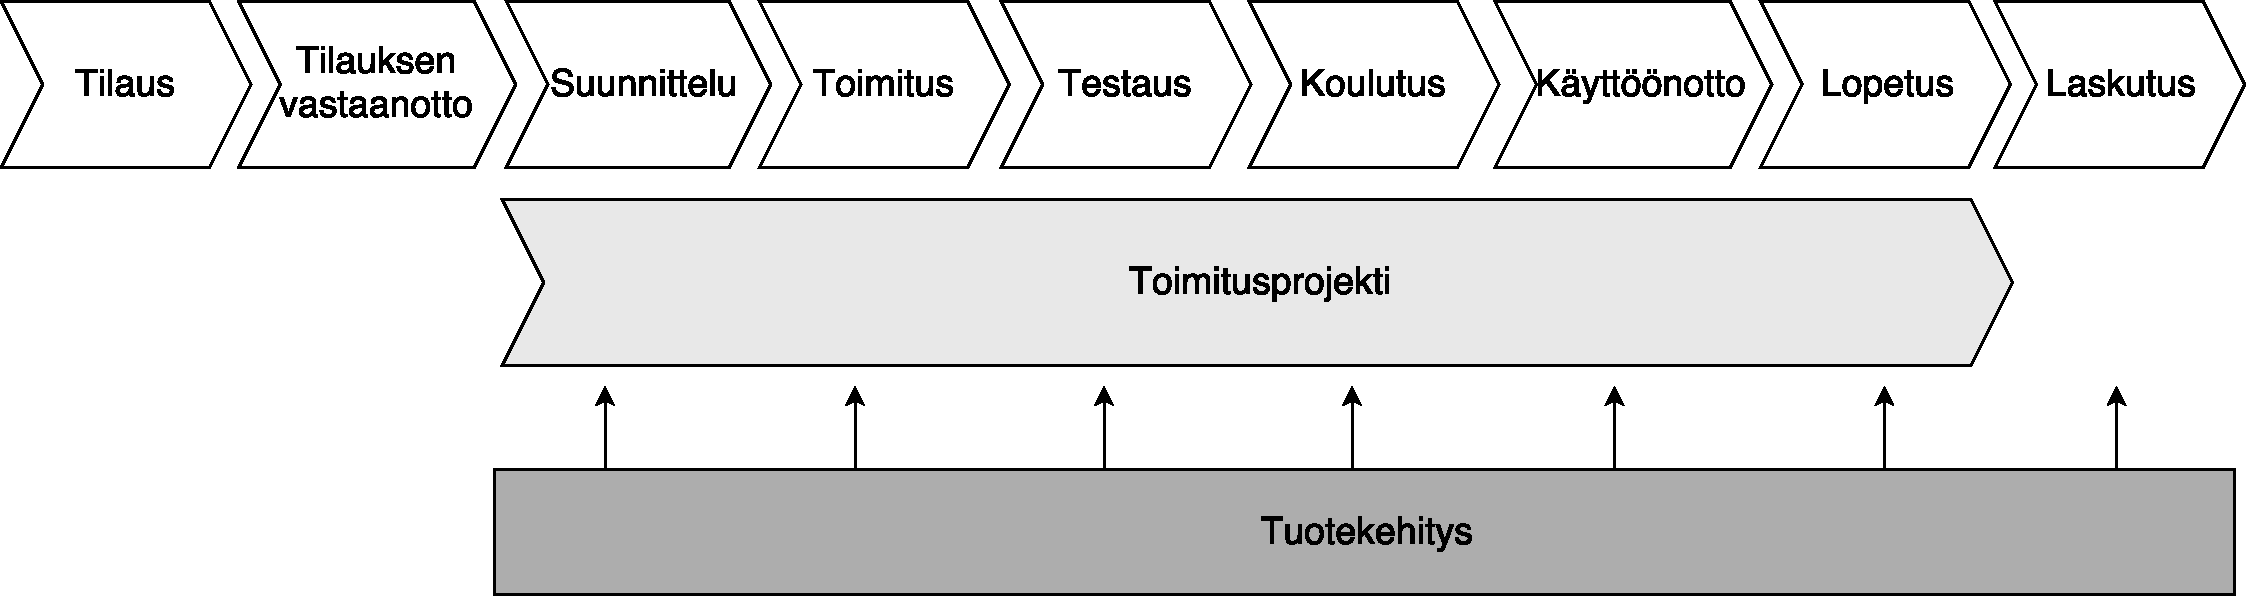
\includegraphics[scale=0.4]{images/ODI-prosessi.pdf}
    \caption{Kontakti L:n asiakasprosessin päävaiheet ja tuotekehitys.}
    \label{fig:paavaih}
\end{figure}

Kontakti L:n asikasprosessi on jaettu kahdeksaan päävaiheeseen. Jokaisesta asiakasprosessin läpikäynnistä muodostetaan asiakaskohtainen toimitusprojekti, johon kuuluu kuusi viimeistä asiakasprosessin vaihetta. Tämän vuoksi jokaisella asiakasprosessin läpikäynnillä on myös oma organisaationsa, joka toimitusprojektissa määritetään. Toimitusprojektia hallinnoi projektipäällikkö, joka vastaa projektisuunnitelman tekemisestä, resurssien hankkimisesta, aikataulutuksesta ja asiakasviestinnästä. Projektipäällikön apuna on tässä toimitusvastaava, joka koordinoi työvaiheissa olevaa tekemistä suunnitelman mukaisesti.\\

Asiakasprosessissa on myös mukana tuotekehityksen tuotepäällikkö ja tuotekehityspäällikkö. Tuotekehityksen rooli on tukea asiakasprosessia tuottamalla vaadittuja järjestelmäkomponentteja ja luoda ohjeistuksia asiakasprosessin eri vaiheisiin. Tuotepäällikkö vastaa Kontkati L:n asiakasprosessista ja sen kehittämisestä. Tuotekehityspäällikkö taas vastaa tuotteen komponenttien kehitystoimenpiteistä alihankkijoiden suuntaan.\\

Kontakti L:n asiakasprosessin päävaiheista ensimmäinen on tilausvaihe. Tilausvaiheeseen tuleva syöte on asiakkaan hyväksymä tarjous. Vaiheen lopputulos on asiakashallinnan järjestelmään muodostuva tilaus asiakkaalle myydystä ratkaisusta. Vaiheen suorittaa ratkaisun myyjä.\\

Asiakashallinnan järjestelmään muodostunut tilaus välittyy tilauksen vastaanottoon, joka on toinen päävaihe. Tilauksen vastaanotossa syötteenä toimii järjestelmässä oleva tilaus yksityiskohtineen. Vaiheessa tarkastetaan täyttävätkö nämä yksityiskohdat tilauksen minimivaatimukset. Lopputuloksena on siis toimituskelpoinen tilaus. Vaiheen toimija on tilauksen vastaanottoon erikoistunut ryhmä.\\

Tilauksen vastaanotto välittää vaatimuksien mukaisen tilauksen kolmanteen asiakasprosessin päävaiheeseen: suunnitteluvaiheeseen. Suunnitteluvaiheen syöte on siis asiakashallinnan järjestelmässä oleva vaatimukset täyttävä tilaus. Vaihe tuottaa lopputuloksena toteutuksen vaatiman projektisuunnitelman, resurssit ja määrittelydokumentit, joiden perusteella toteutus tehdään. Tässä vaiheessa toimijoita on useampia: Projektipäällikkö käynnistää toimitusprojektin, hallinnoi sitä ja tekee projektisuunnitelman. Toimitusvastaava koordinoi ja tekee toteutukseen liittyviä valmistelutöitä. Tuotekehitys taas tukee toimitusprojektia tuottamalla tilauksessa olevia uusia komponentteja ja ohjeistuksia toteutusta varten. Suunnittelijat ovat myös mukana tuottamassa itse määrittelydokumentit seuraavaan vaiheeseen. Myös itse toteutuksen tekevät järjestelmäasiantuntijat ovat mukana saamassa ohjeistusta toteutusta varten.\\

Projektisuunnitelma, resurssivaraukset ja määrittelydokumentit toimivat syötteenä toimitusvaiheelle, joka on päävaiheista neljäs. Näiden perusteella toimitusvaihe toteuttaa lopputuloksena Kontakti L-järjestelmäratkaisun, joka vastaa asiakkaan tilausta. Toimijoina tässä vaiheessa on erilaiset ratkaisun komponentteihin erikoistuneet järjestelmäasiantuntijat, joiden tekemistä toimitusprojekti koordinoi. Alihankkijan järjestelmäasiantuntijat asentavat Kontakti L-järjestelmän. Telian järjestelmäasiantuntijat taas tekevät asiakkaan vaatimat konfiguroinnit ja integraatiot. \\

Viidennen asiakasprosessin päävaiheen, eli testausvaiheen syöte on asiakkaan tilauksen perusteella tuotettu Kontakti L-järjestelmäratkaisu. Testausvaiheessa todennetaan, että ratkaisu vastaa Telian laatuvaatimuksia ja asiakkaan tarpeita. Testausvaiheen lopputuloksena on siis asiakkaan vaatimuksia vastaava viestintäratkaisu. Tässä vaiheessa toimijoina ovat Telialta puhesuunnittelija ja järjestelmäasiantuntija. Asiakas myös suorittaa hyväskymistestauksen tässä vaiheessa.\\

Kontakti L-järjestelmän ollessa toimintavalmiina alkaa koulutusvaihe, joka on päävaiheista kuudes. Koulutusvaiheen syöte on asiakkaan tilauksessa määritetty käyttäjien koulutus. Vaiheen tuloksena asiakkaan käyttäjillä on tarvittavat valmiudet käyttää järjestelmää. Toimijana tässä vaiheessa on Telian Kontakti L-järjestelmän koulutustiimi.\\

Seitsemäs asiakasprosessin päävaihe on käyttöönottovaihe. Vaiheen syöte on testattu Kontakti L-järjestelmä, jota koulutuksen saaneet asiakkaan käyttäjät alkavat käyttää. Vaiheessa varmistetaan, että ratkaisu vastaa asiakkaan tarvetta käytännössä ja varaudutaan tekemään hienosäätöä. Vaiheen lopputuloksena Kontakti L-järjestelmä on käytössä asiakkaan haluamalla tavalla. Vaiheen toimijoina ovat Telialta järjestelmäasiantuntijat ja asiakas.\\

Viimeisessä kahdeksannessa päävaiheessa syötteenä toimii käynnissä oleva toimitusprojekti, joka lopetetaan tämän vaiheen seurauksena. Toimijana vaiheessa on projektipäällikkö, toimitusvastaava ja tuotantopäällikkö.





Kontakti L:n asiakasprosessi alkaa ratkaisun myyjän tekemästä tilauksesta, josta se välittyy tilauksen vastaanottoon. Tilauksen vastaanotossa toimii määrätyt henkilöt joiden tehtävä on varmistaa, että tilaus täyttää Kontakti L:n tilauksen minimivaatimukset. Tilauksen vastaanotto välittää minimivaatimukset täyttävän tilauksen Telian projektitoimiston työjonoon, josta alkaa suunnitteluvaihe.\\

Projektitoimiston esimies siirtää työjonosta tilauksen vastuutetulle projektipäällikölle. Projektipäällikön tehtävä on aloittaa toimitusprojekti ja valvoa projektin kulkua. Suunnitteluvaiheessa toimitusprojektin aloittamiseksi, projektipäällikön on käytävä tilaus läpi ja selvittää sen perusteella mitä resursseja toimitusprojekti tarvitsee. Projektipäällikön apuna toimitusprojektissa ovat toimitusvastaavat, jotka koordinoivat yksittäisten toimitettavien komponenttien toimitusta prosessissa.\\

Kun projektin vaatimat resurssit on hankittu, jatkuu suunnitteluvaihe puhe- ja IP-suunnittelijan tekemällä ratkaisun määrittelyllä. Määrittelyn tuloksena saadaan dokumentit, joiden avulla toimitusvaihe voi alkaa. Toimitusvaiheeseen päästään kun Kontakti L:n toimitusvastaava suorittaa ensin valmistelut toimitusta ja laskutusta varten. Toimitusvastaava tilaa projektipäällikön varamilta resursseilta toimituksen vaatimat työt, jolloin toimitusvaihe alkaa. Suunnittelu- ja toimitusvaihe tapahtuvat osin päällekäin.\\

Toimitusvaiheen alussa Tiedon työntekijä asentaa palvelimille vaaditut järjestelmän komponentit toimitusvastaavan tilauksesta ja käyttää suunnitteluvaiheessa luotuja määrittelydokumentteja. Kun asennus on kuitattu valmiiksi, toimitusvastaava tilaa järjestelmän konfigurointityön resurssivarauksen mukaiselta Telian järjestelmäasiantuntijalta, joka jälleen tekee vaadittavat konfiguroinnit ja integraatiot määrittelydokumenttien perusteella. Kun työ kuitataan valmiiksi alkaa ratkaisun testausvaihe.\\

Testausvaiheeseen ei ole toistaiseksi määritelty ohjeistusta, jonka mukaan testaus tulisi tehdä. Haastatteluiden perusteella testausta on kuitenkin tehnyt edellisen vaiheen järjestelmäasiantuntija ja puhesuunnittelija. Kun on todettu, että järjestelmä on toiminnassa alkaa koulutusvaihe.\\

Koulutusvaiheessa resurssivarauksen mukaisen kouluttajat aikatauluttavat ja suunnittelevat asiakkaalle tehtävät koulutukset toimitusvastaavan tilauksen perusteella. Kouluttajat opettavat asiakkaan käyttäjiä järjestelmän käytössä ja varmistavat, että käyttäjillä on tarvittavat kyvyt ja tukimateriaali kun järjestelmä otetaan käyttöön. Koulutusvaiheen jälkeen Kontakti L on valmiina käyttöönottoon. Koulutusvaihe ja käyttöönottovaihe tapahtuvat osin samanaikaisesti.\\

Käyttöönottovaiheessa projektipäällikkö ja toimitusvastaava sopivat aikataulun asiakkaan kanssa käyttöönoton ajasta. Aluksi asiakas tekee järjestelmän hyväksymistestauksen oman ohjeistuksensa mukaan. Telian järjestelmäasiantuntija tukee ohjeistuksen mukaan asiakasta käyttöönotossa. Kun asiakas on ottanut järjestelmän käyttöön, alkaa toimitusprojektin lopetusvaihe.\\

Lopetusvaiheessa projektipäällikkö käynnistää asiakkaan laskutuksen ja vapauttaa resurssivaraukset toimitusprojektilta. Viimeisessä laskutusvaiheessa tuotepäällikkö aloittaa Kontakti L:n kuukausilaskutuksen ja laskuttaa myös toimitusvaiheen työt asiakkaalta. Asiakasprosessi päättyy tähän.\\

Tuotekehitys on mukana asiakasprosessissa suunnitteluvaiheesta asti tukemalla muiden sidosryhmien työvaiheita ja koordinoimalla asiakasprosessissa esiin noussseita kehitystöitä alihankkijoilta.

 

- Asiakas
- Myyjä
- Tilausten vastaanottaja
- Projektitoimisto
- Projektipäällikkö
- Toimitusvastaava
- Tuotepäällikkö
- Tuotekehityspäällikkö
- Tieto L3
- Zylinc
- Tuotantopäälliköt
- Puhesuunnittelija
- IP-suunnittelija
- L2 konfiguroija
- Kouluttaja
- Tallentaja

Muut prosessit:
-RaVa-prosessi
-Datanet/SPVA-toimitusprosessi
-Mobiilitoimituksen prosessi
-Tuotekehitysprosessi
-Ylläpitoprosessi

Järjestelmät
- Tellu
- MultiBella
- Tiksu


\subsubsection{Prosessin läpikäynti}

Tässä osiossa käymme läpi Kontakti L:n asiakasprosessin kulun vaihe kerrallaan. Ensin käydään läpi yksittäisen vaiheen kulku, ja samalla kuvataan vaiheen riippuvuutta muihin prosessin vaiheisiin. Kuvauksessa tuodaan esiin vaiheen toimijat, dokumentit ja järjestelmät. Tämän osion tavoite on antaa tarkka kuva Kontakti L:n asiakasprosessin toiminnasta. \\

\textbf{Tilausvaiheen kulku}\\

%Vaiheen kesto on arvioitu olevan noin 1 päivä.\\

Kontakti L:n asiakasprosessi alkaa myyjän tekemästä tilauksesta, ja tämä vaihe on kuvattu kuvassa \ref{fig:tilaus}. Tätä ennen asiakas on hyväksynyt tarjouksen ja myyjä on varmistanut asiakaspalvelujärjestelmän toimitusajan erillisen ratkaisun varmistus-prosessin kautta. Ratkaisun varmistus-prosessia käytetään, koska Kontakti L:n asiakasprosessi ei ole vielä valmiina toimitukseen kehitysvaiheessa. Saatuaan päätöksen toimitusajasta, myyjä tekee palvelusopimuksen asiakkaan kanssa, jonka liitteeksi lisätään palvelutasosopimus, palvelun yksityiskohtaiset tiedot sisältävän palvelukuvauksen, palvelun hinnaston ja toimitusehdot.

\begin{figure}[!h]
    \centering
    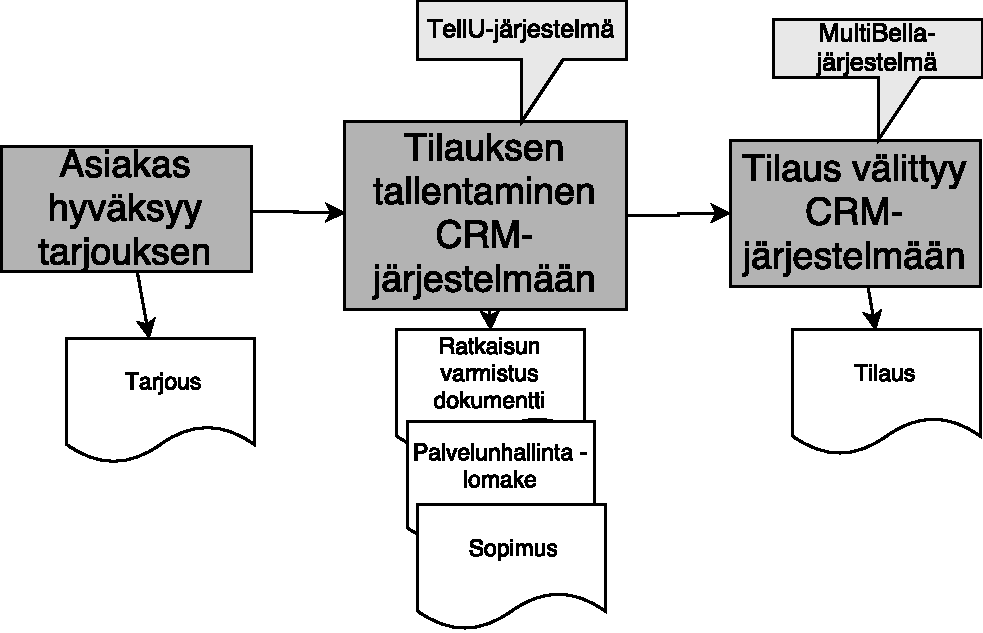
\includegraphics[scale=0.4]{images/tilaus.pdf}
    \caption{Kontakti L:n asiakasprosessin tilausvaihe.}
    \label{fig:tilaus}
\end{figure}

Kun sopimusosapuolet ovat allekirjoittaneet sopimuksen, myyjä tekee tilauksen Tellu-järjestelmän kautta, jossa tilaus tehdään lomakepohjaisen verkkosivun kautta. TellU-järjestelmä on Telian myynnin käytössä oleva asiakashallinnan järjestelmä. Tilauksen mukaan myyjä liittää varmennusprosessin tekemän päätöksen toimitusajasta, sopimuksen ja täytetyn palvelunhallintalomakkeen. Palvelunhallintalomake on Excel-tiedosto, jossa on valmis lomake-pohja myydyn asiakaspalvelujärjestelmän tietoja varten. Myyjän tehtyä tilauksen, välittyy se automaattisesti toiseen Telian käyttämään asiakashallinnan järjestelmään nimeltä MultiBella.\\

\textbf{Tilausten vastaanotto-vaiheen kulku}\\

%Vaiheen kesto on arvioitu olevan noin 1 päivä.\\

Tilauksen vastaanotto-vaihe alkaa kun tilauksen vastaanotossa työskentelevä henkilö ottaa tilauksen käsittelyyn työjonostaan MultiBella-järjestelmässä. Henkilö tekee tilaukselle esitarkistuksen. Esitarkastuksen ensimmäisessä vaiheessa asiantuntija tarkastaa, että tilauksen mukana on hyväksytty päätös ratkaisun toimitusajasta. Toisessa vaiheessa hän tarkastaa, että tilauksesta löytyy minimivaatimukset.\\

\begin{figure}[!h]
    \centering
    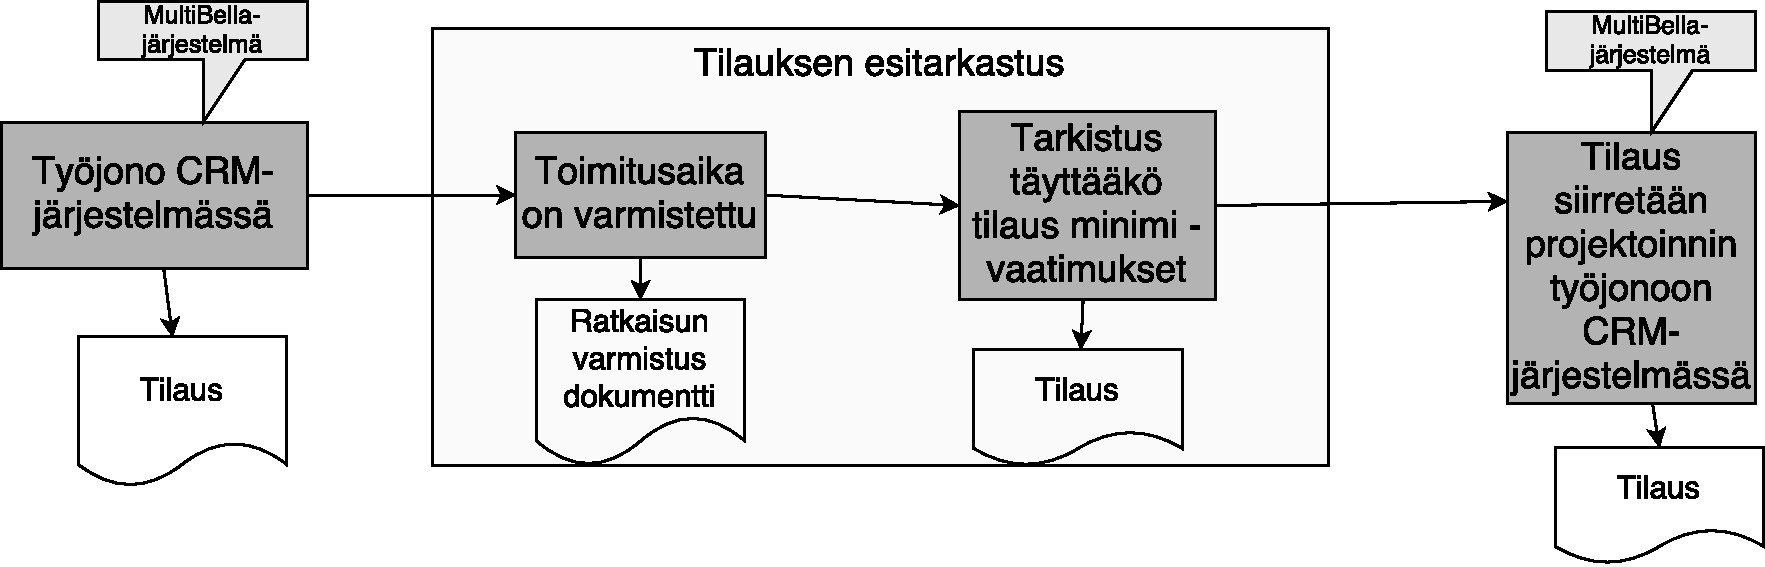
\includegraphics[scale=0.4]{images/tilvast.pdf}
    \caption{Kontakti L:n asiakasprosessin tilauksen vastaanotto-vaihe.}
    \label{fig:tilausvast}
\end{figure}

Minimivaatimukset täyttävä tilaus sisältää: palvelun lisenssien ennakoidut kappalemäärät, mahdolliset integraatioit muihin palveluihin ja sopimuksen yksikköhinnat. Asiantuntija siirtää minimivaatimukset täyttävän tilauksen projektitoimiston työjonoon MultiBella-järjestelmässä, jolloin tilauksen vastaanotto-vaihe päättyy\\

\textbf{Suunnitteluvaihe}\\

%Vaiheen kesto on arvioitu olevan noin 1-2 kuukautta.\\

\begin{figure}[!h]
    \centering
    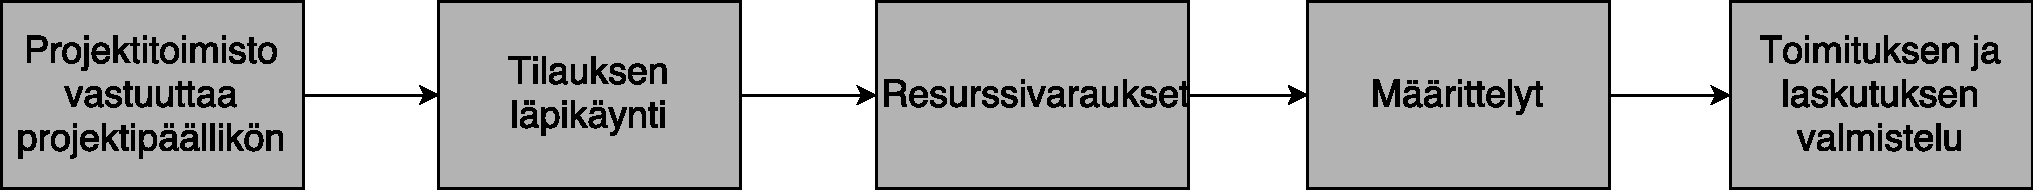
\includegraphics[scale=0.35]{images/ykssuunn.pdf}
    \caption{Kontakti L:n asiakasprosessin yksinkertaistettu suunnitteluvaihe.}
    \label{fig:ykssuun}
\end{figure}

Toimituksen suunnitteluvaihe käsittää asiakastoimituksen valmisteluun liittyvät työvaiheet: Toimitusprojektin aloitustoimet, jossa tilauksen sisältö tarkastetaan. Projektin resurssivaraukset, eli ihmiset, jotka tekevät seuraavat työvaiheet. Ratkaisuun liittyvän määrittelytyön. Viimeisenä toimituksen ja laskutuksen valmistelun. Tämän vaiheen tuloksena on projektisuunnitelma ja määrittelydokumentit. Käsitellään näitä neljää suunnitteluvaiheen osasta erillään.\\

\textbf{Suunnitteluvaihe: Tilauksen läpikäynti}\\

Suunnitteluvaiheen aloitustoimiin päästään kun projektitoimiston esimies on vastuuttanut projektipäällikön Kontakti L:n toimitusprojektille MultiBella-järjestelmän tilauksen perusteella. Kuvassa \ref{fig:aloitustoimet} on esitettynä tämä osuus suunnitteluvaiheesta. Projektipäällikkö käynnistää toimitusprojektin hankkimalla sille projektinumeron ProofX-järjestelmässä, johon kustannukset voidaan kohdentaa. Tämän jälkeen hän järjestää tapaamisen Kontakti L:n tuotepäällikön ja tuotekehityspäällikön kanssa tilauksen läpikäymiseksi. \\

\begin{figure}[!h]
    \centering
    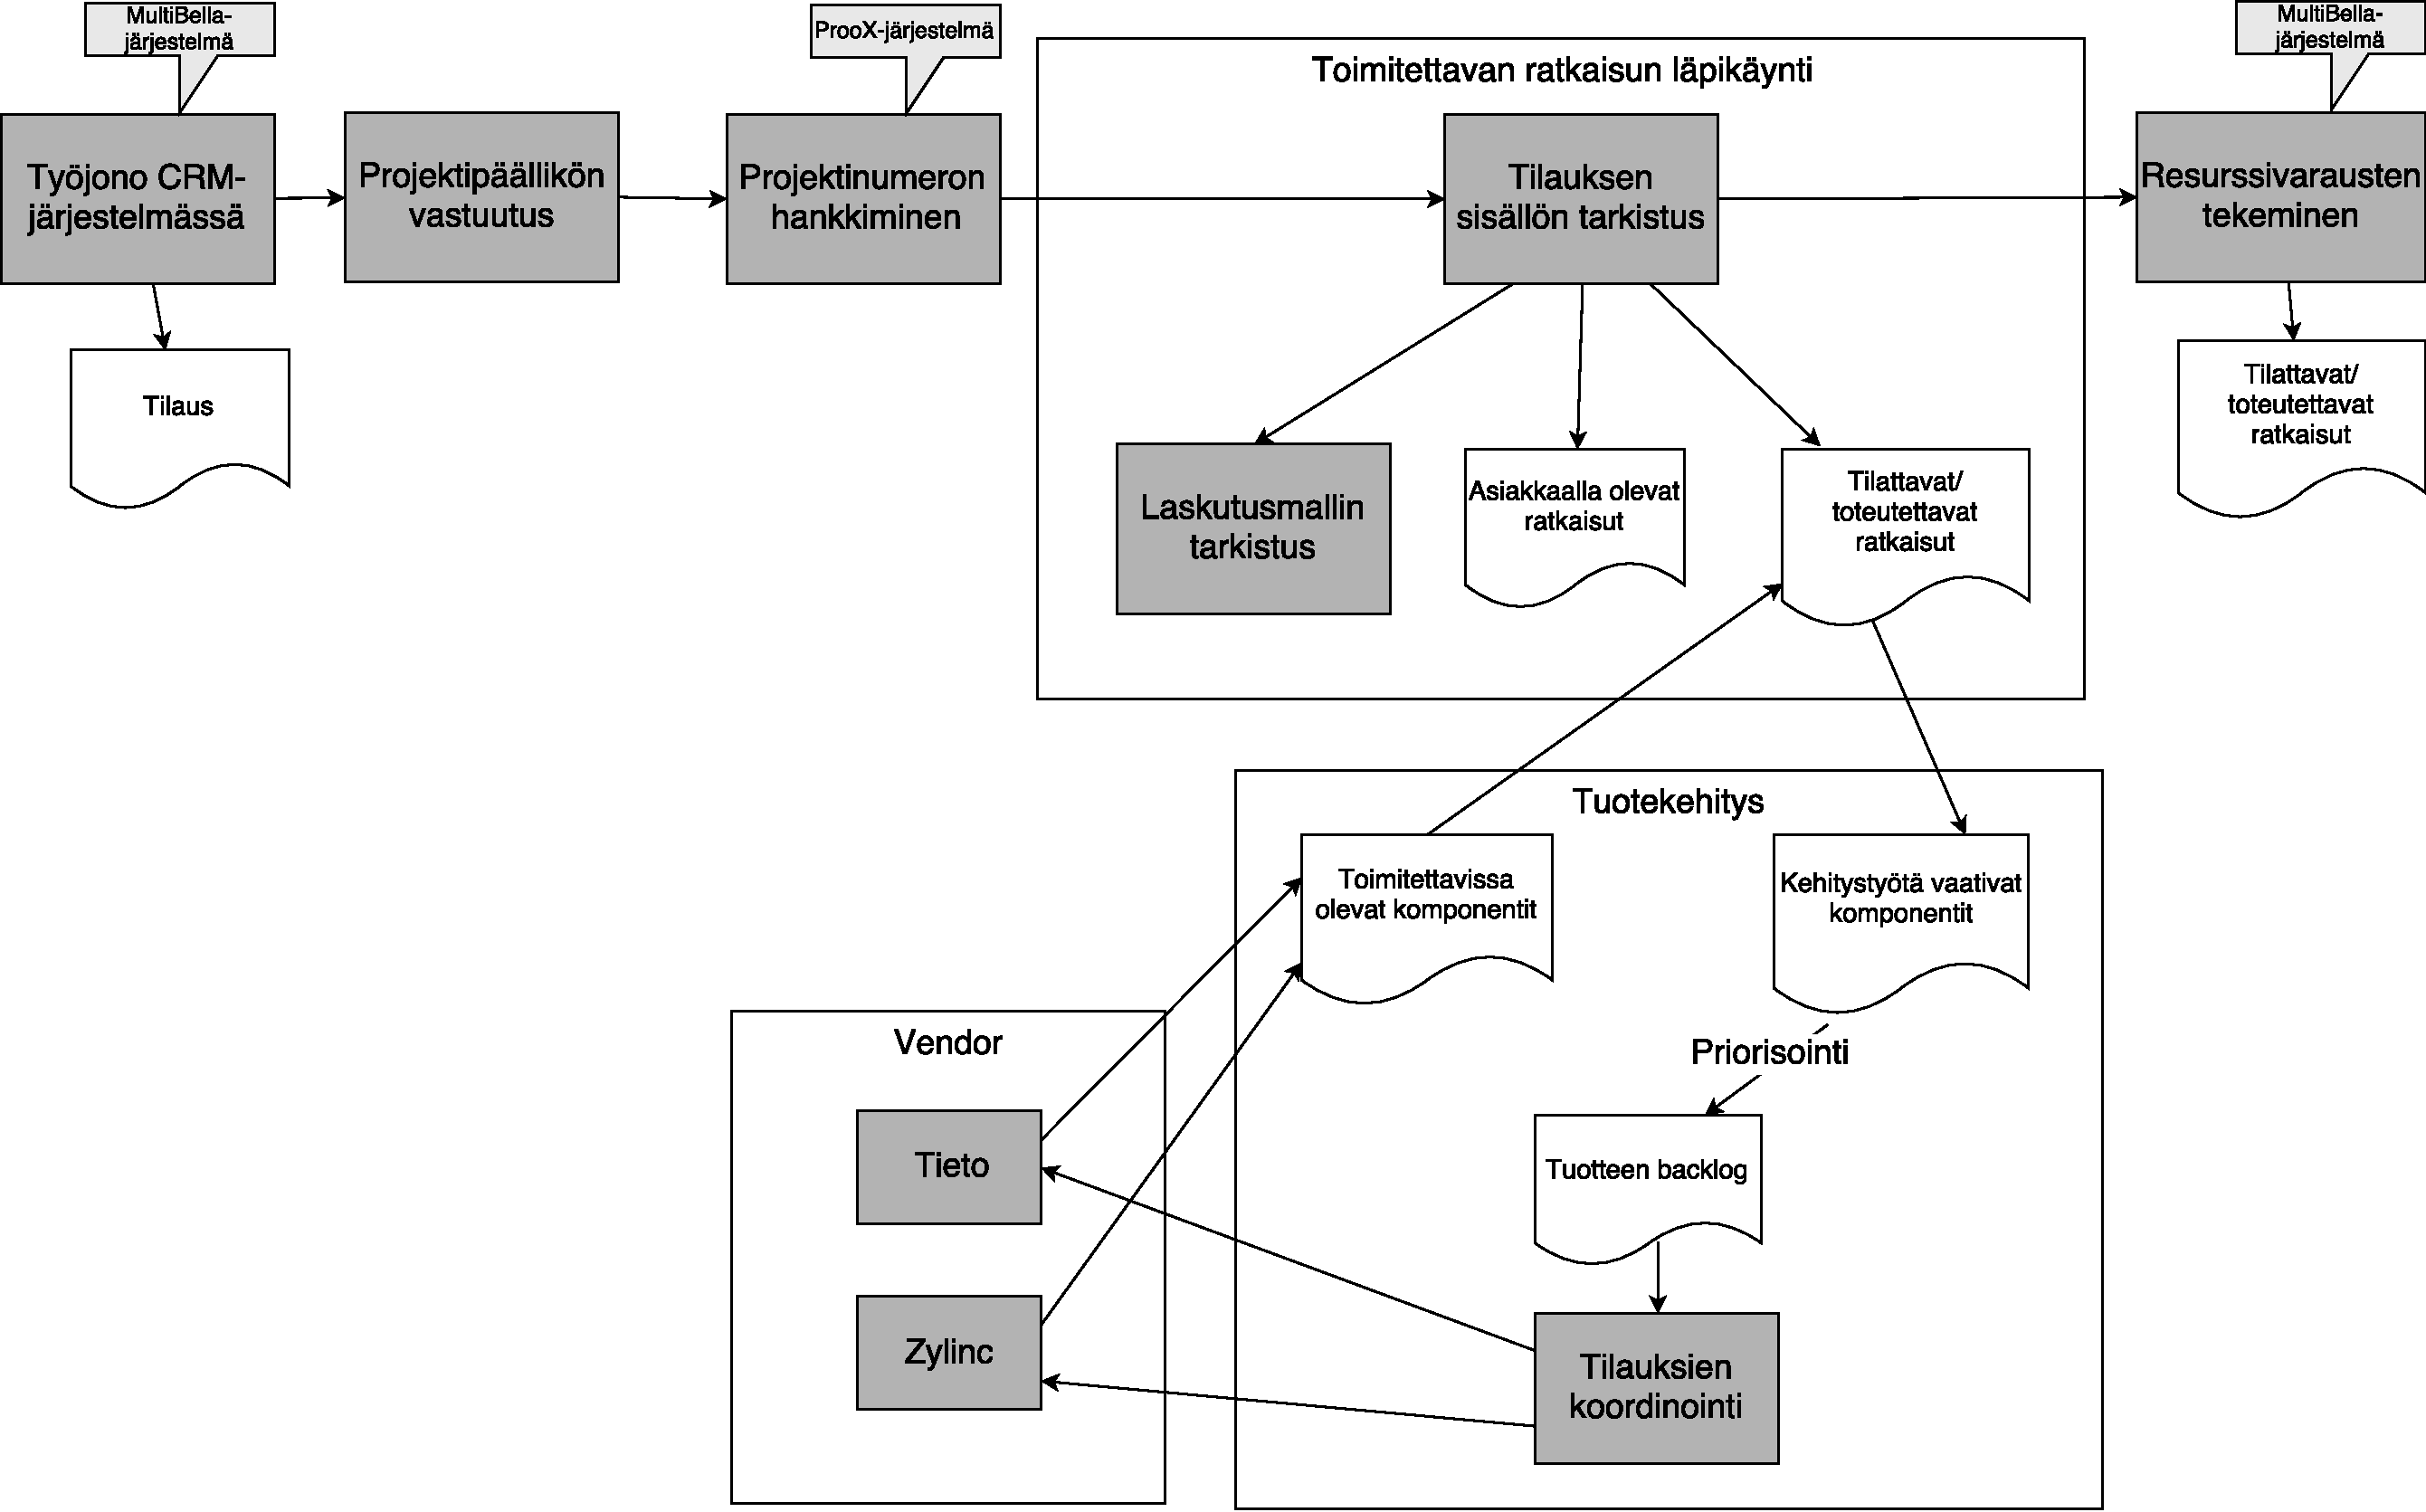
\includegraphics[scale=0.3]{images/aloitus.pdf}
    \caption{Kontakti L:n asiakasprosessin suunnitteluvaiheen tilauksen läpikäynti.}
    \label{fig:aloitustoimet}
\end{figure}

Tapaamisessa tilauksesta tarkistetaan minkälaista laskutusmallia asiakkaan kanssa tulisi käyttää, mitä viestintäratkaisuun kuuluvia komponentteja asiakkaalla jo on käytössä, ja mitä viestintäratkaisun komponentteja asiakkaalle tulee tilauksen perusteella toimittaa.\\

Kun toimitettavat komponentit ovat tunnistettu, jaetaan ne kahteen kategoriaan: Komponentteihin jotka on toimitettavissa ja kehitystyötä vaativiin komponentteihin. Toimitettavilla komponenteilla on resurssi, jolla on siihen liittyvä osaaminen ja ohjeistus. Kehitystyötä vaativat komponentit asetetaan tuotteen backlogiin priorisoidusti muiden siellä jo olevien komponenttien kanssa.\\

Kontakti L:n tuotepäällikkö ja tuotekehityspäällikkö priorisoivat backlogissa olevia komponentteja, ja tilaavat niihin liittyvän toteutuksen alihankkijalta. Se kumpaa alihankkijaa käytetään riippuu vaaditusta kehitystyöstä. Tieto tekee Telian palvelinalustaan liittyvät toimenpiteet ja Zylinc itse tuotteeseen liittyvän kehitystyön.\\

Kun toimitettavat komponentit on tunnistettu ja kehitystyötä vaativien komponenttien aikataulu on selvillä, tekee projektipäällikkö näiden komponenttien toimittamiseen liittyvät resurssivaraukset.\\

\textbf{Suunnitteluvaihe: Resurssivaraukset}\\

Toimitettavien komponenttien perusteella projektipäällikkö aloittaa resurssivarausten tekemisen. Kuvassa \ref{fig:resurssit} on esitettynä resurssivarausten osat. Ensimmäisenä projektipäällikkö tilaa Datanet-yhteyden asiakkaalle Tomaatti-järjestelmän kautta jos asiakkaalla ei vielä olemassaolevaa yhteyttä. Seuraavaksi hän tekee toimitusvastaavan resurssivarauksen MultiBella-järjestelmän kautta, ja sopii hänen kanssaan roolit toimitusprojektin ajaksi.\\

\begin{figure}[!h]
    \centering
    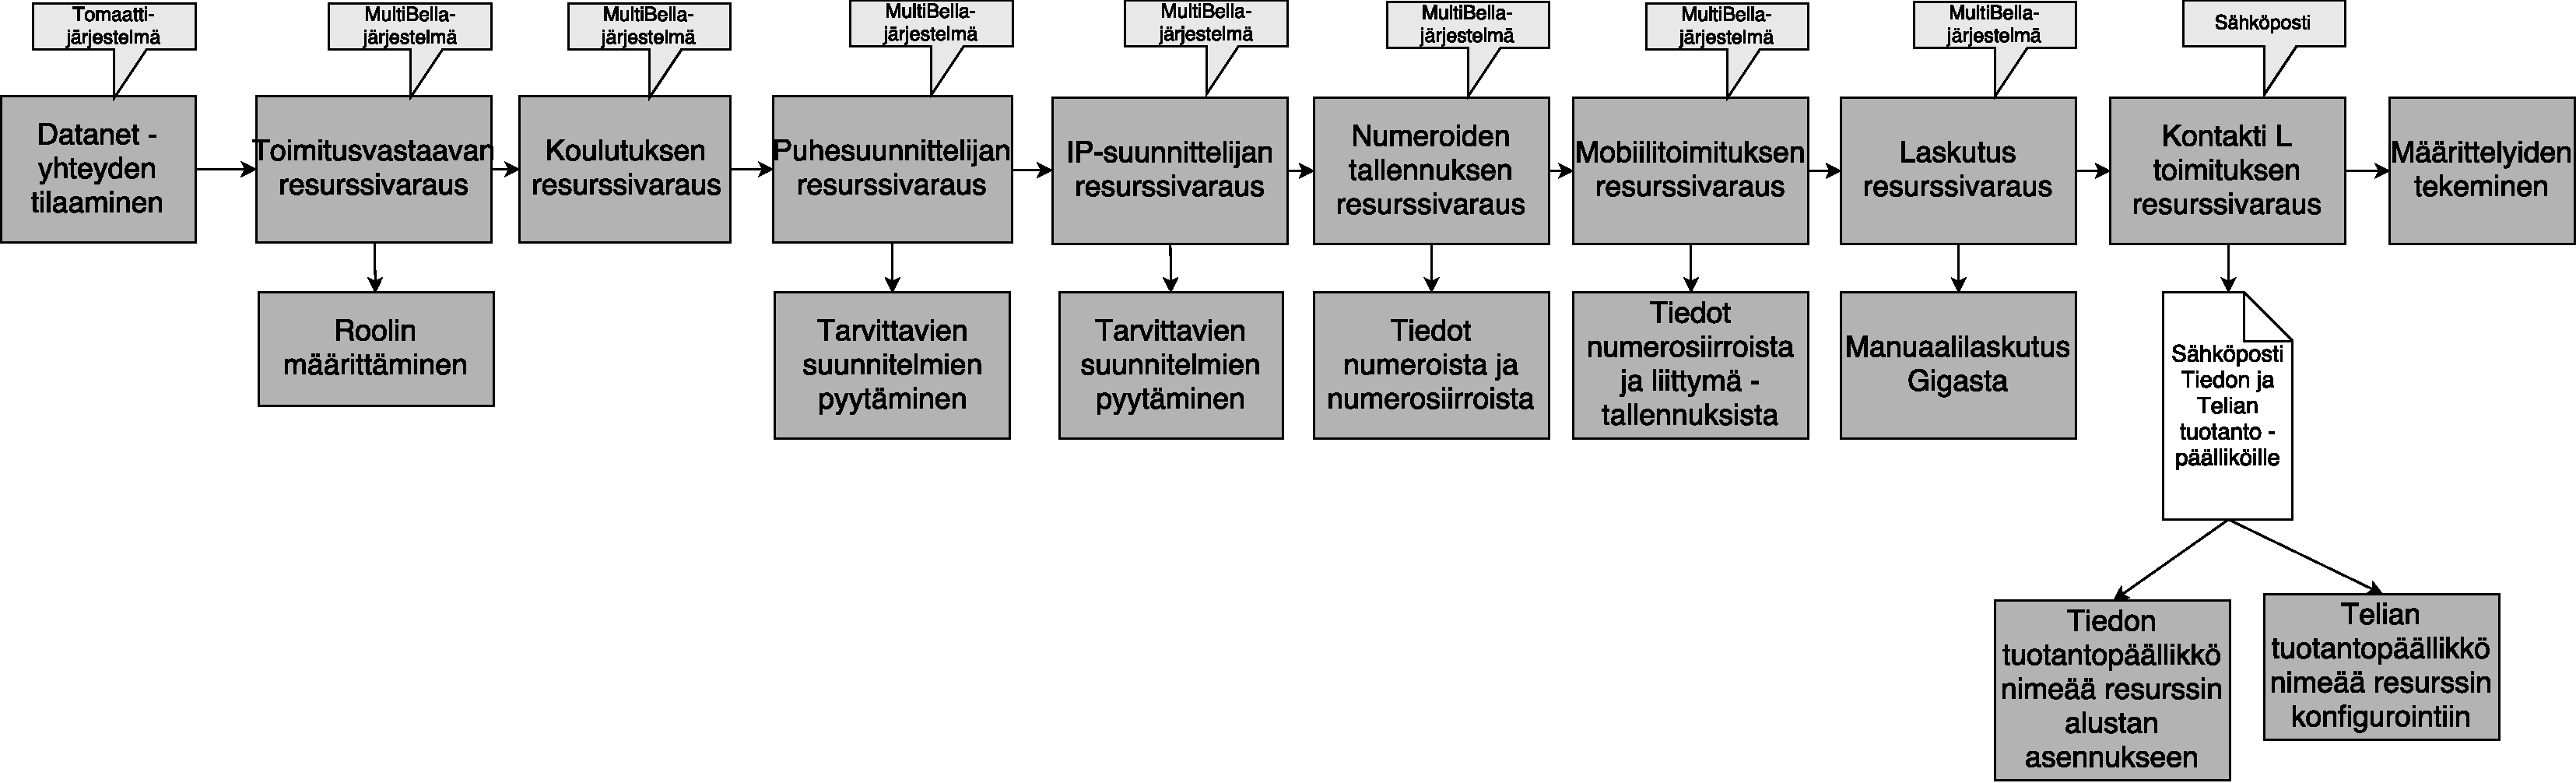
\includegraphics[scale=0.25]{images/resurssivaraukset.pdf}
    \caption{Kontakti L:n asiakasprosessin suunnitteluvaiheen resurssivaraukset.}
    \label{fig:resurssit}
\end{figure}

Tämän jälkeen projektipäällikkö tarkastaa sopimuksessa vaaditun koulutustarpeen, ja tekee sen perusteella resurssivarauksen MultiBella-järjestelmästä. Sen jälkeen hän varaa resurssin puhe- ja IP-suunnitteluun ja pyytää heiltä sopimuksessa mainitut suunnitelmat ratkaisun toimittamiseksi.\\

Seuraavaksi projektipäällikkö varaa resurssin palvelunumeroiden ja mobiilinumeroiden toimituksilta, ja välittää heille tiedot ratkaisussa käytetyistä numeroista, numerosiirroista ja uusien liittymien avaamisesta. Laskutuksen henkilöresurssin varaaminen on toistaiseksi epäselvää, ja sen vuoksi Kontakti L:n tuotepäällikön vastuulla. Toistaiseksi tuotepäällikkö on hoitanut laskutuksen itse manuaalisesti Giga-laskutusjärjestelmästä. Laskutuksen resurssia kuitenkin tarvitaan uuden yrityksen luomisessa, joten resurssi varataan silloin MultiBella-järjestelmästä joko tuotepäällikön tai projektipäällikön toimesta.\\

Viimeiseksi projektipäällikkö varaa resurssit järjestelmän asennukseen ja konfigurointiin lähettämällä sähköpostin Tiedon ja Telian järjestelmäasiantuntijoiden esimiehille eli tuotantopäälliköille. Tuotantopäälliköt nimeävät resurssit tehtäviinsä vastaamalla tähän sähköpostiin.\\

Kun kaikki resurssivaraukset on tehty, päästään aloittamaan ratkaisun määrittelytyö.\\

\textbf{Suunnitteluvaihe: Määrittelyt}\\

Kuvassa \ref{fig:maarittely} on esitettynä suunnitteluvaiheen määrittelyt. Ratkaisun määrittelytyö alkaa projektipäällikön järjestämässä tapaamisessa asiakkaan edustajien kanssa, jossa on mukana toimitusprosessissa olevat resurssit. Tapaamisen tarkoitus on tarkentaa tilauksen tietoja, sopia yhteisistä toimintamalleista, yhteyshenkilöistä ja aikataulusta. Tämän tapaamisen jälkeen projektipäällikkö järjestää vielä toisen tapaamisen sisäisesti toimitusorganisaation kanssa.\\

\begin{figure}[!h]
    \centering
    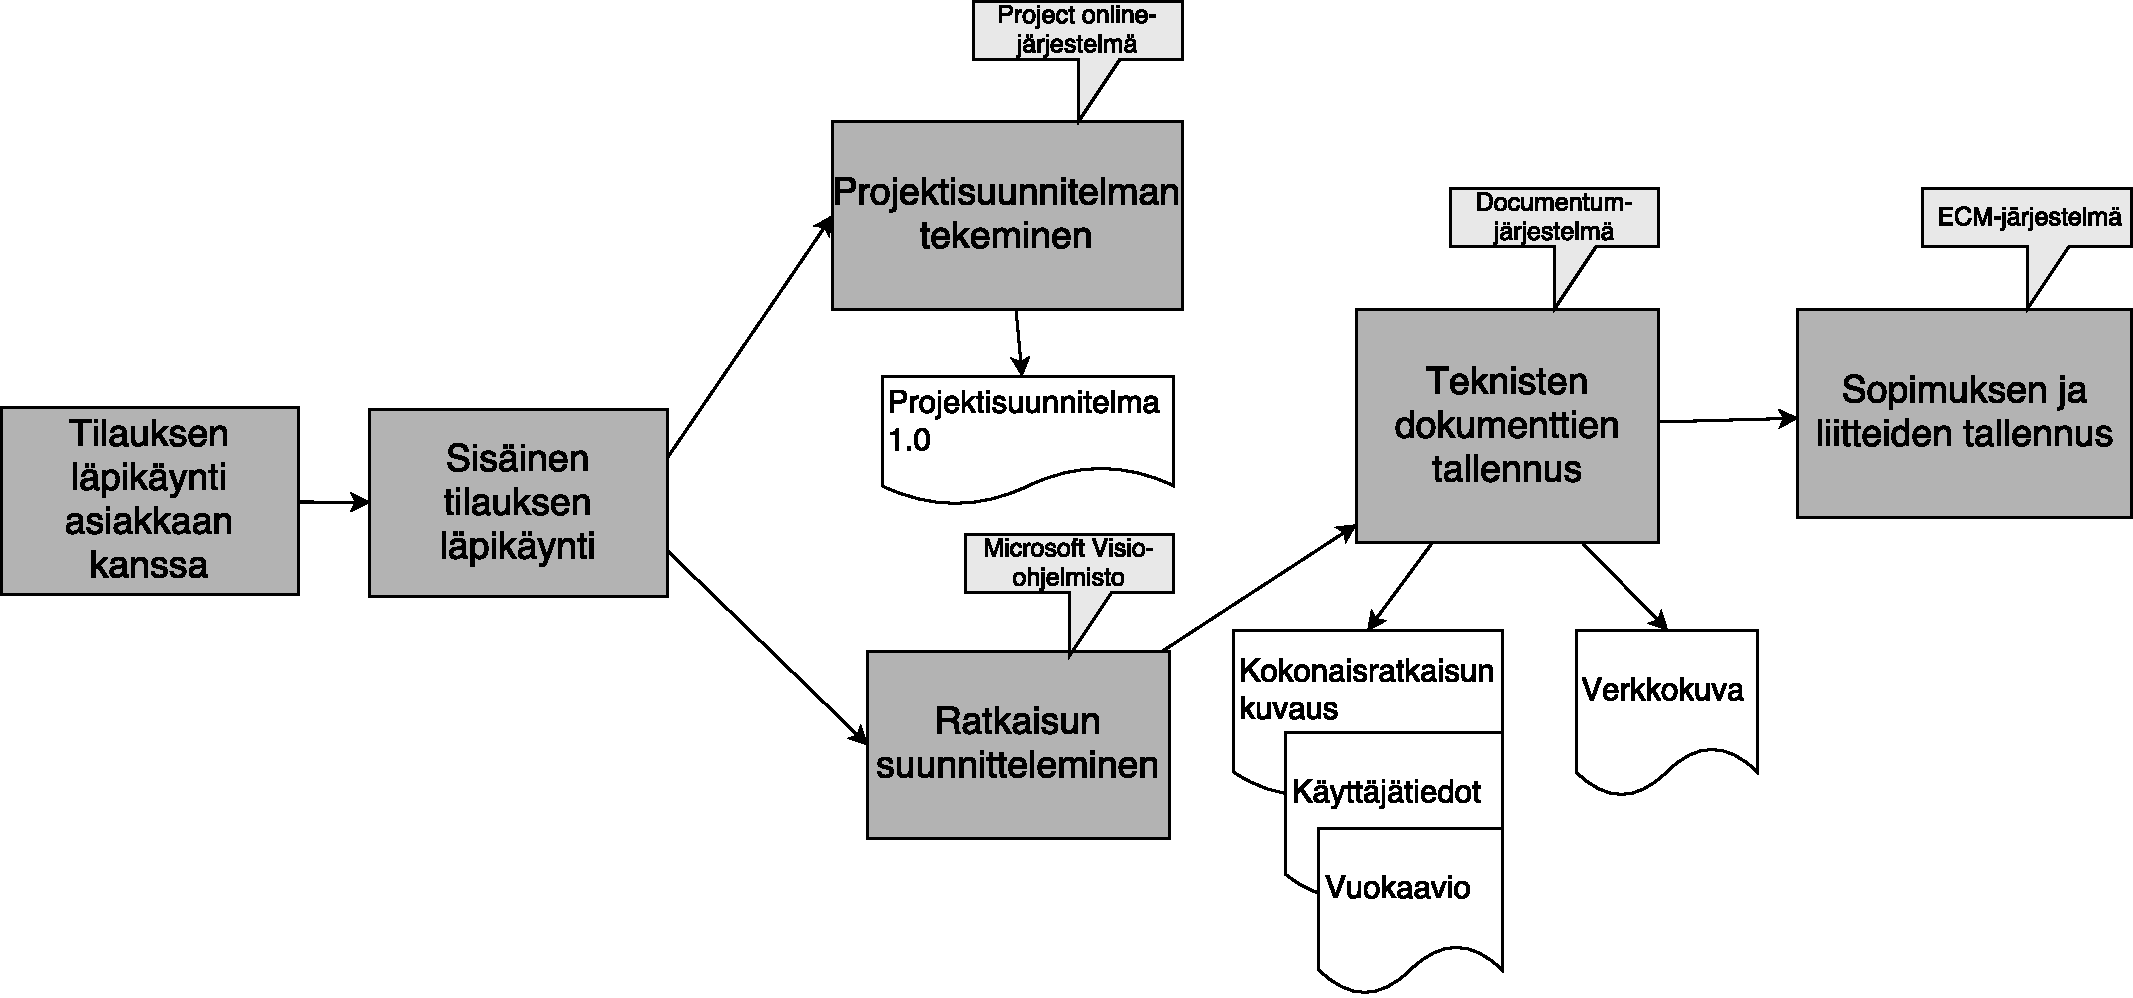
\includegraphics[scale=0.25]{images/maarittely.pdf}
    \caption{Kontakti L:n asiakasprosessin suunnitteluvaiheen määrittelyt.}
    \label{fig:maarittely}
\end{figure}

Kun yhteisistä toimintamalleista on sovittu, projektipäällikkä tekee projektisuunnitelman ensimmäisen version Project online projektisuunnittelujärjestelmässä. Samanaikaisesti puhesuunnittelija ja IP-suunnittelija aloittavat ratkaisun suunnittelun. He suunnittelevat ratkaisun yhteistyössä asiakkaan yhteyshenkilöiden kanssa. Suunnittelutyö dokumentoidaan Microsoft Visio-ohjelmalla. Puhesuunnittelijan työn tuloksena syntyy kuvaus kokonaisratkaisuista ja sen eri komponenteista ja vuokaavio ratkaisun numeroista, jonoista ja komponenteista. Puhesuunnittelija myös kerää asiakkaan käyttäjätiedot. IP-suunnittelijan työn tuloksena syntyy verkkokuva, josta ilmenee ratkaisun yhteydet, IP-osoitteet ja verkot. Suunnittelijat tallentavat dokumentit Documentum versiohallinnan järjestelmään.\\

Lopuksi toimitusvastaava vie sopimuksen liitteineen ECM-järjestelmään. Jo tämän vaiheen aikana toimitusvastaava on aloittanut toimituksen ja laskutuksen valmistelun.\\ 

\textbf{Suunnitteluvaihe: Toimituksen ja laskutuksen valmistelu}\\

Jo määrittelyiden tekemisen aikana toimitusvastaava aloittaa valmistelemaan toimitusta ja laskutusta. Kuvassa \ref{fig:valmtoimlask} on esitettynä tämän vaiheen kulku. Tämä vaihe on osittain päällekäinen toimitusvaiheen kanssa.

\begin{figure}[!h]
    \centering
    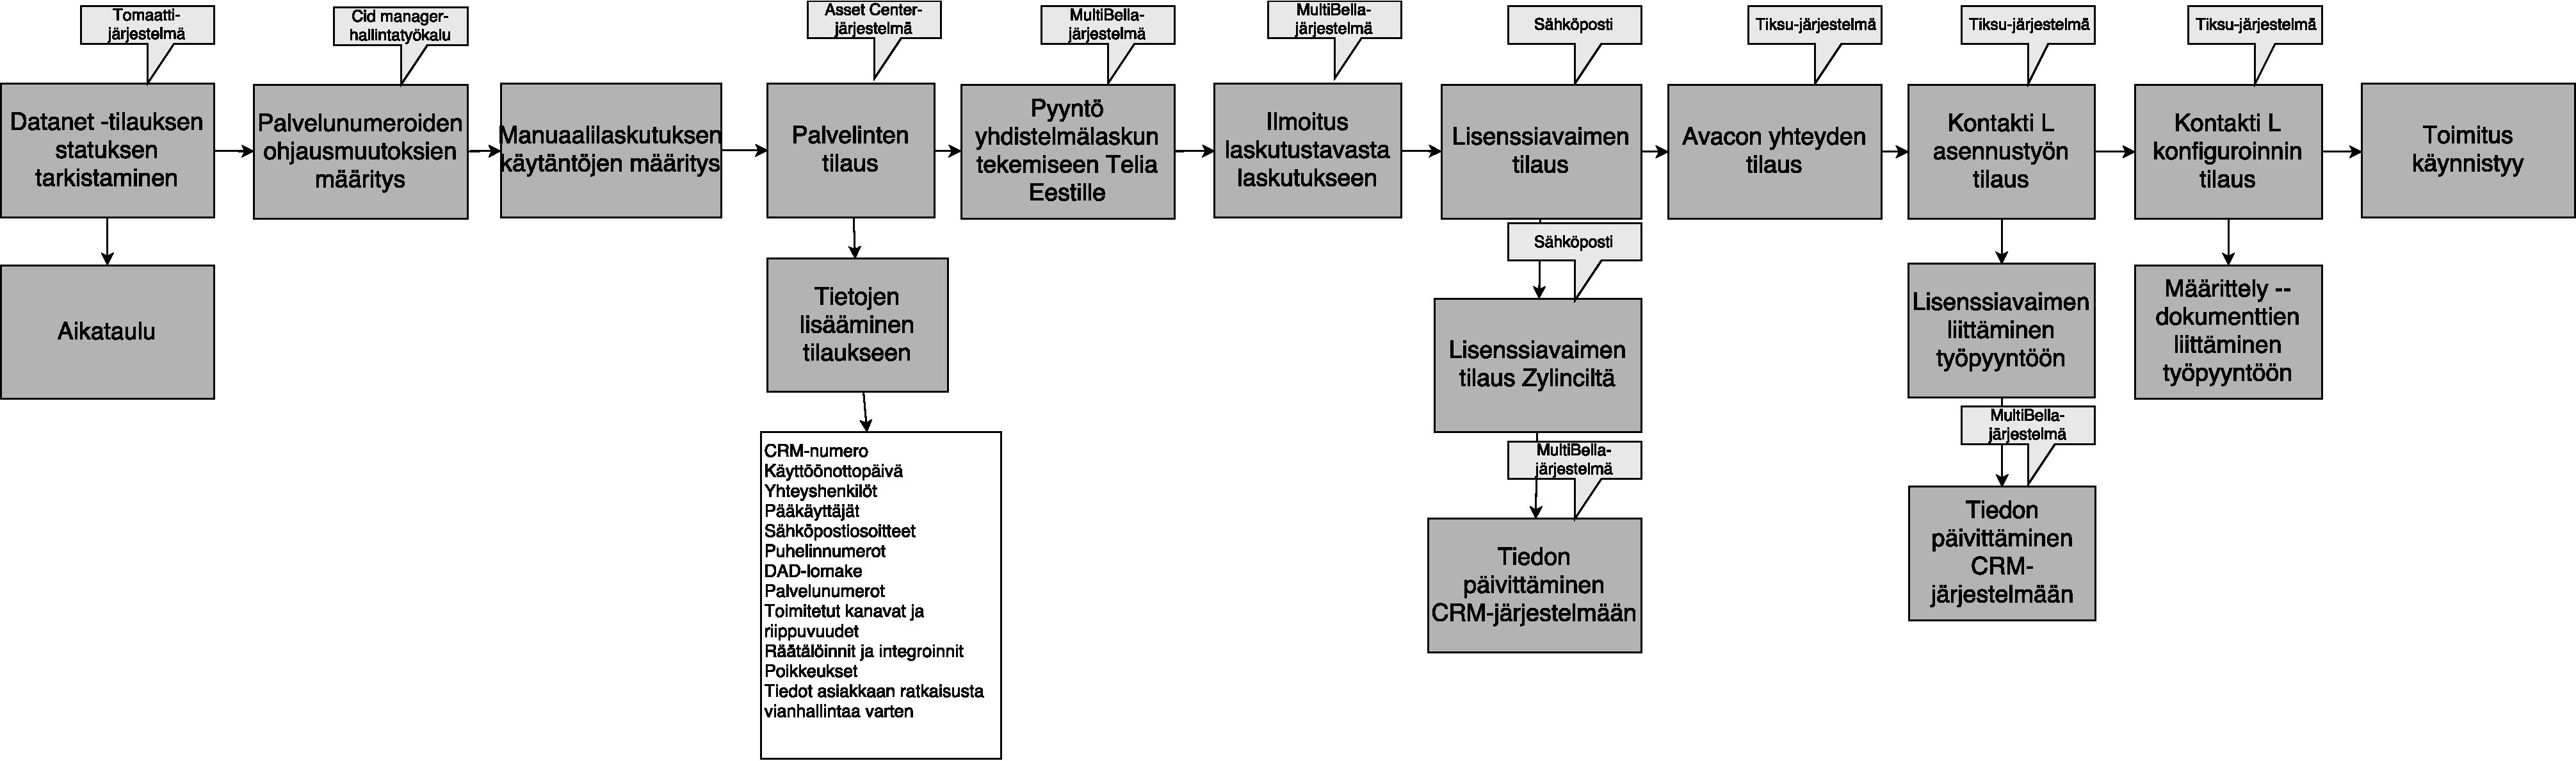
\includegraphics[scale=0.2]{images/valmtoimlask.pdf}
    \caption{Kontakti L:n asiakasprosessin suunnitteluvaiheen toimituksen ja laskutuksen valmistelu.}
    \label{fig:valmtoimlask}
\end{figure}

Ensimmäinen toimitusvastaavan tehtävä on seurata Datanet-yhteyksien toimitusta ja saada aikataulu sen valmistumisesta, koska toimitusvaihe ei voi alkaa ennen yhteyksien saamista. Tämän jälkeen hän tekee asiakkaan palvelunumeroista ohjausmääritykset valmiiksi Cid manager numeroiden hallintatyökalun kautta odottamaan toimitusta. Toimitusvastaava käy myös seuraavaksi läpi manuaalilaskutuksen käytännöt Kontakti L:n tuotepäällikön kanssa, että hänellä on tarvittavat tiedot laskutustavasta ja yhdistelmälaskun tilaamisesta asiakkaalle.\\

Tämän jälkeen toimitusvastaava tilaa Kontakti L:n palvelimet Asset Center-järjestelmästä, ja lisää tietoihin kuvassa näkyvät tiedot asiakkaan ratkaisusta vianhallintaa varten. Sitten hän tekee MultiBella-järjestelmässä työpyynnön Telia Eestille yhdistelmälaskun tekemisestä asiakkaalle ja ilmoittaa laskutustavan Suomen laskutukseen.\\

Seuraavaksi toimitusvastaava pyytää sähköpostitse Kontakti L:n tuotekehityspäällikköä tilaamaan lisenssiavaimen järjestelmään Zylinciltä ja päivittää tiedon tästä MultiBella-järjestelmään. Tuotekehityspäällikkö tilaa lisenssiavaimen sähköpostitse Zylinciltä. Palvelinten ollessa valmiina, toimitusvastaava tilaa Tiksu tiketöintijärjestelmästä etäyhteydet toimitusta varten. Etäyhteyksien toimiessa, hän lähettää Tiksu-järjestelmästä työpyynnön Tiedolle Kontakti L:n asennusta varten ja liittää sähköpostista lisenssiavaimen liitteeksi.\\

Kun Tieto on kuitannut asennuksen valmistuneen, päivittää toimitusvastaava tiedon Multibella-järjestelmään. Seuraavaksi hän tilaa Kontakti L:n konfigurointi ja integrointityön Telian järjestelmäasiantuntijalta Tiksu-järjestelmän kautta ja liittää määrittelydokumentit työpyynnön liitteeksi.\\

Toimitusvastaava seuraa työvaiheiden toteutumista ja päivittää tiedot MultiBella-järjestelmään. Tämä seuranta kuuluu osaltaa jo seuraavaan toimitusvaiheeseen asiakasprosessia.\\

\textbf{Toimitusvaihe}\\

%Vaiheen kesto on arvioitu olevan noin 2-4 kuukautta.\\

Tämä vaihe on esitetty kuvassa \ref{fig:toimitus}. (Ei toistaiseksi tarkempaa tietoa yhteyksien toimituksesta) Toimitusvaihe alkaa kun Datanet-toimitus saa Tiksu-järjestelmästä työpyynnön yhteyksien toimittamisesta. Työpyynnön liitteenä on IP-suunnittelijan tekemä verkkokuva, jonka perusteella yhteydet toimitetaan. Työn valmistuessa asiantuntija kuittaa Tiksu-järjestelmän työpyynnön valmiiksi.\\

\begin{figure}[!h]
    \centering
    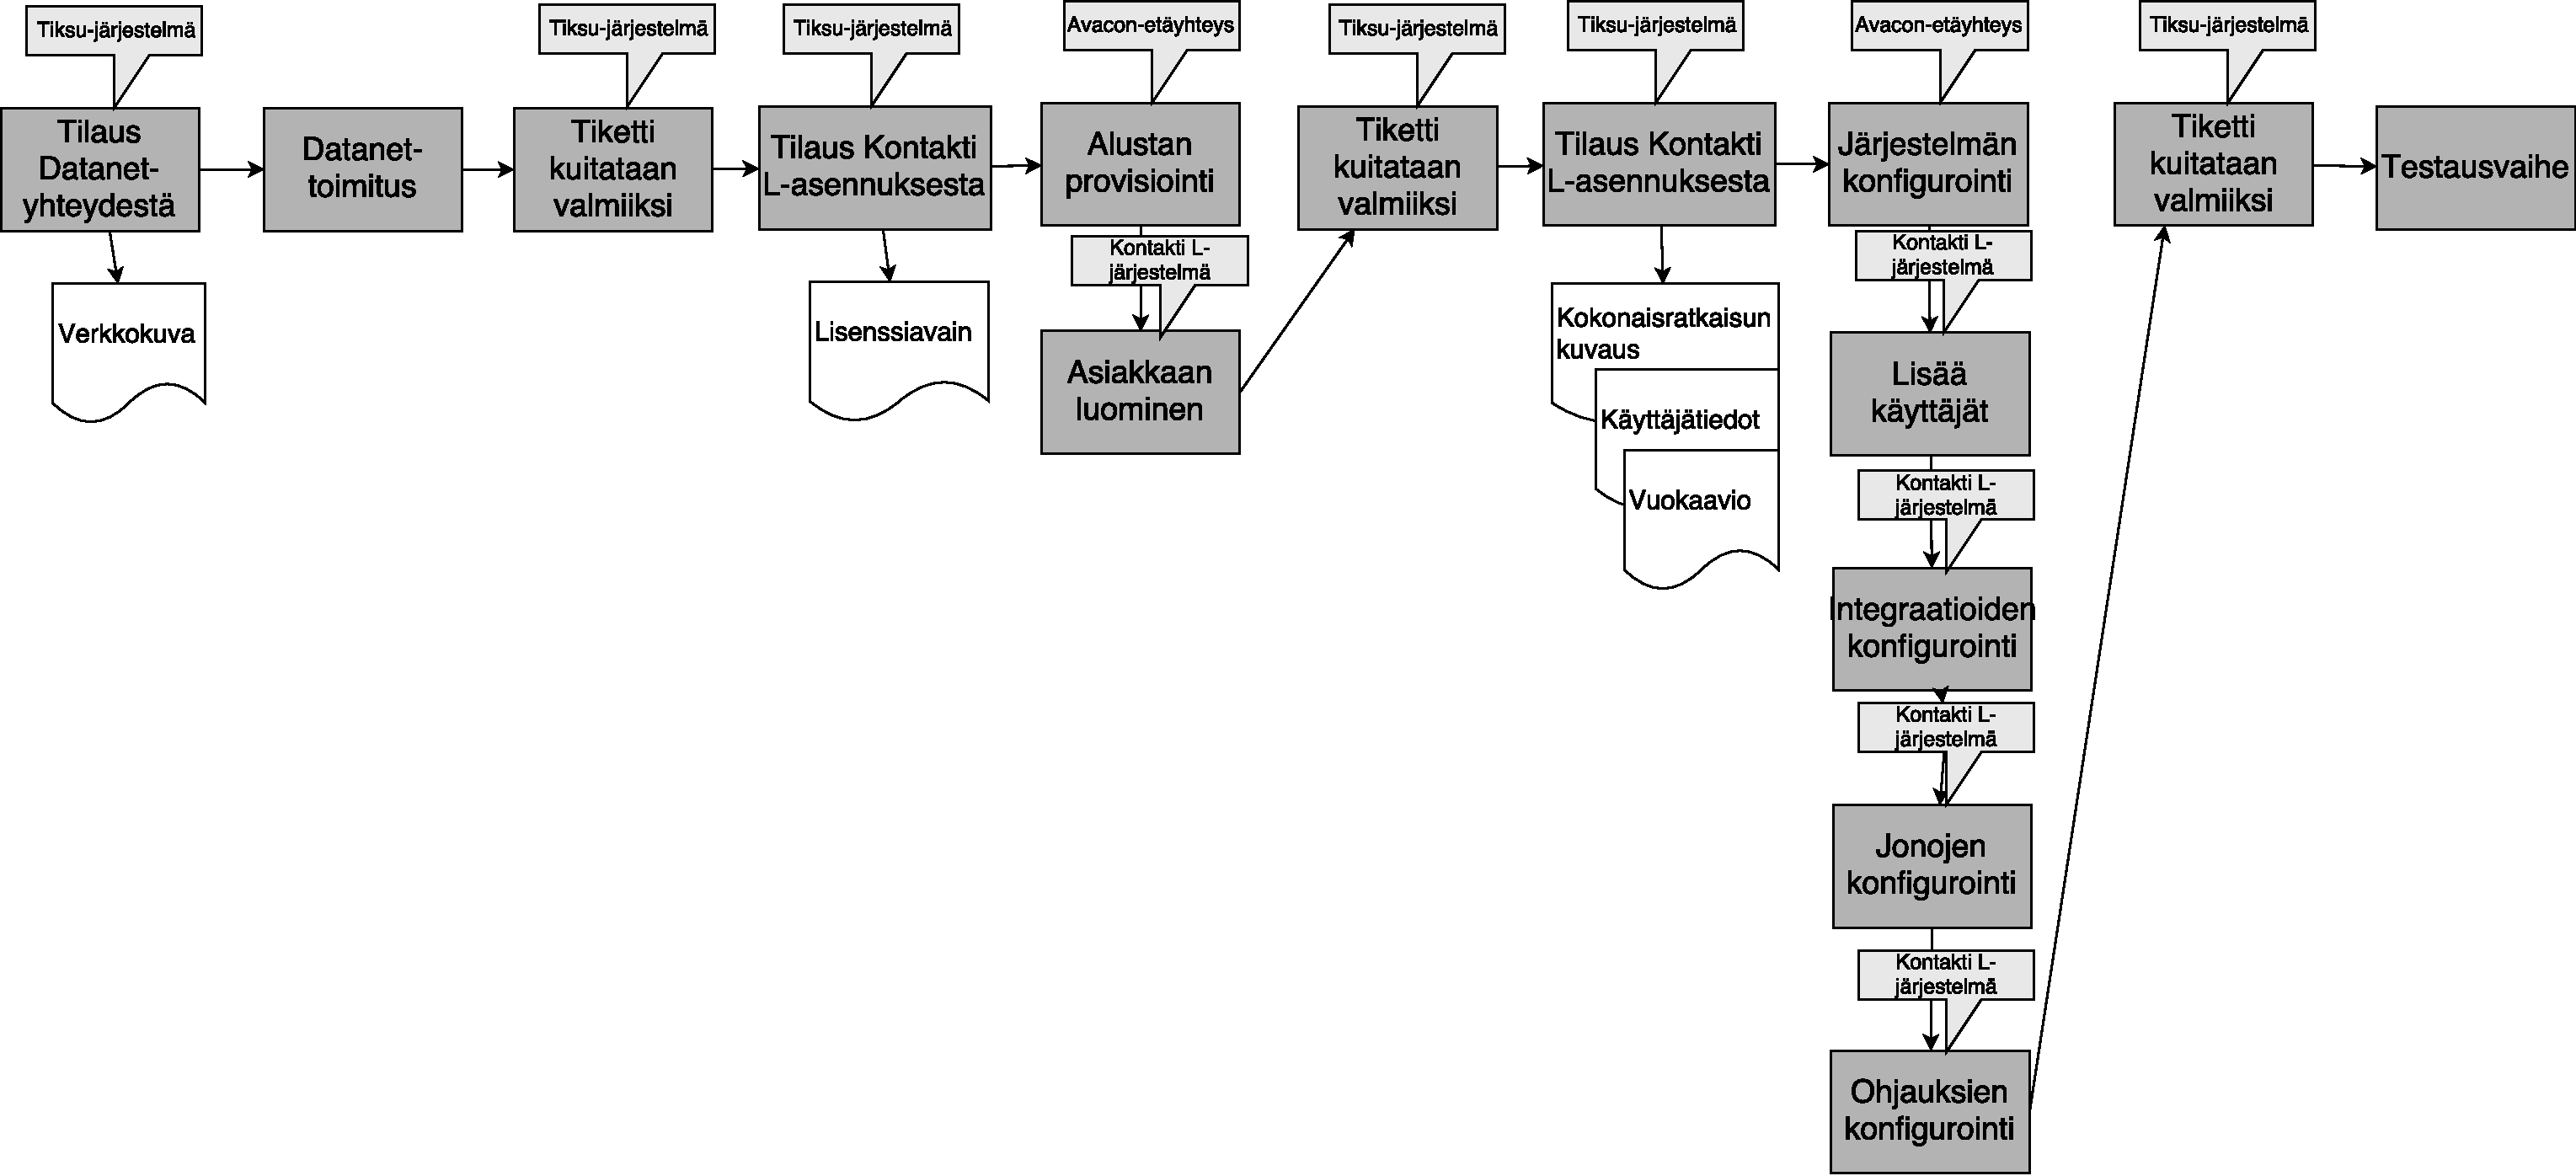
\includegraphics[scale=0.3]{images/toimitus.pdf}
    \caption{Kontakti L:n asiakasprosessin toimitusvaihe.}
    \label{fig:toimitus}
\end{figure}

Tämän jälkeen Tiedon järjestelmäasiantuntija saa työpyynnön Tiksu-järjestelmässä Kontakti L:n asennuksesta, jonka liitteenä on järjestelmän lisenssiavain. Järjestelmäasiantuntija asentaa Kontakti L:n palvelimelle Avacon-etäyhteyden avulla, ja kuittaa tämän jälkeen työpyynnön valmiiksi Tiksu-järjestelmässä.\\

Tämän jälkeen Telian järjestelmäasiantuntija saa työpyynnön Tiksu-järjestelmässä Kontakti L:n konfigurointi- ja integrointityöstä. Työpyynnön liitteenä on ratkaisun määrittelydokumentit ja käyttäjätiedot. Järjestelmäasiantuntija ottaa Avacon-etäyhteyden Kontakti L-palvelimelle. Ensin hän lisää käyttäjätiedon Kontakti L-järjestelmään, ja sen jälkeen tekee tarvittavat integroinnit. Kun integraatiot toimivat, alkaa järjestelmäasiantuntija konfiguroimaan jonoja ja kontaktien ohjaustietoja järjestelmään. Kun kaikki integraatiot ja konfiguroinnit on todettu toimiviksi, järjestelmäasiantuntija kuittaa Tiksu-järjestelmän työpyynnön valmiiksi.\\

Tämän jälkeen alkaa Kontakti L-järjestelmän testausvaihe.\\

\textbf{Testausvaihe}\\

%Vaiheen kesto on arvioitu olevan noin 1-2 viikkoa.\\

Testivaiheen kulku on esitetty kuvassa \ref{testaus}. Testaus alkaa testinumeroiden kytkemisellä Kontakti L-järjestelmään. Testinumerot varataan ja niihin liittyvät kytkennät pyydetään tehtäväksi Atlas-järjestelmän kautta. Kun kytkennät on tehty, voidaan ne asettaa käyttöön Kontakti L-järjestelmässä. \\

\begin{figure}[!h]
    \centering
    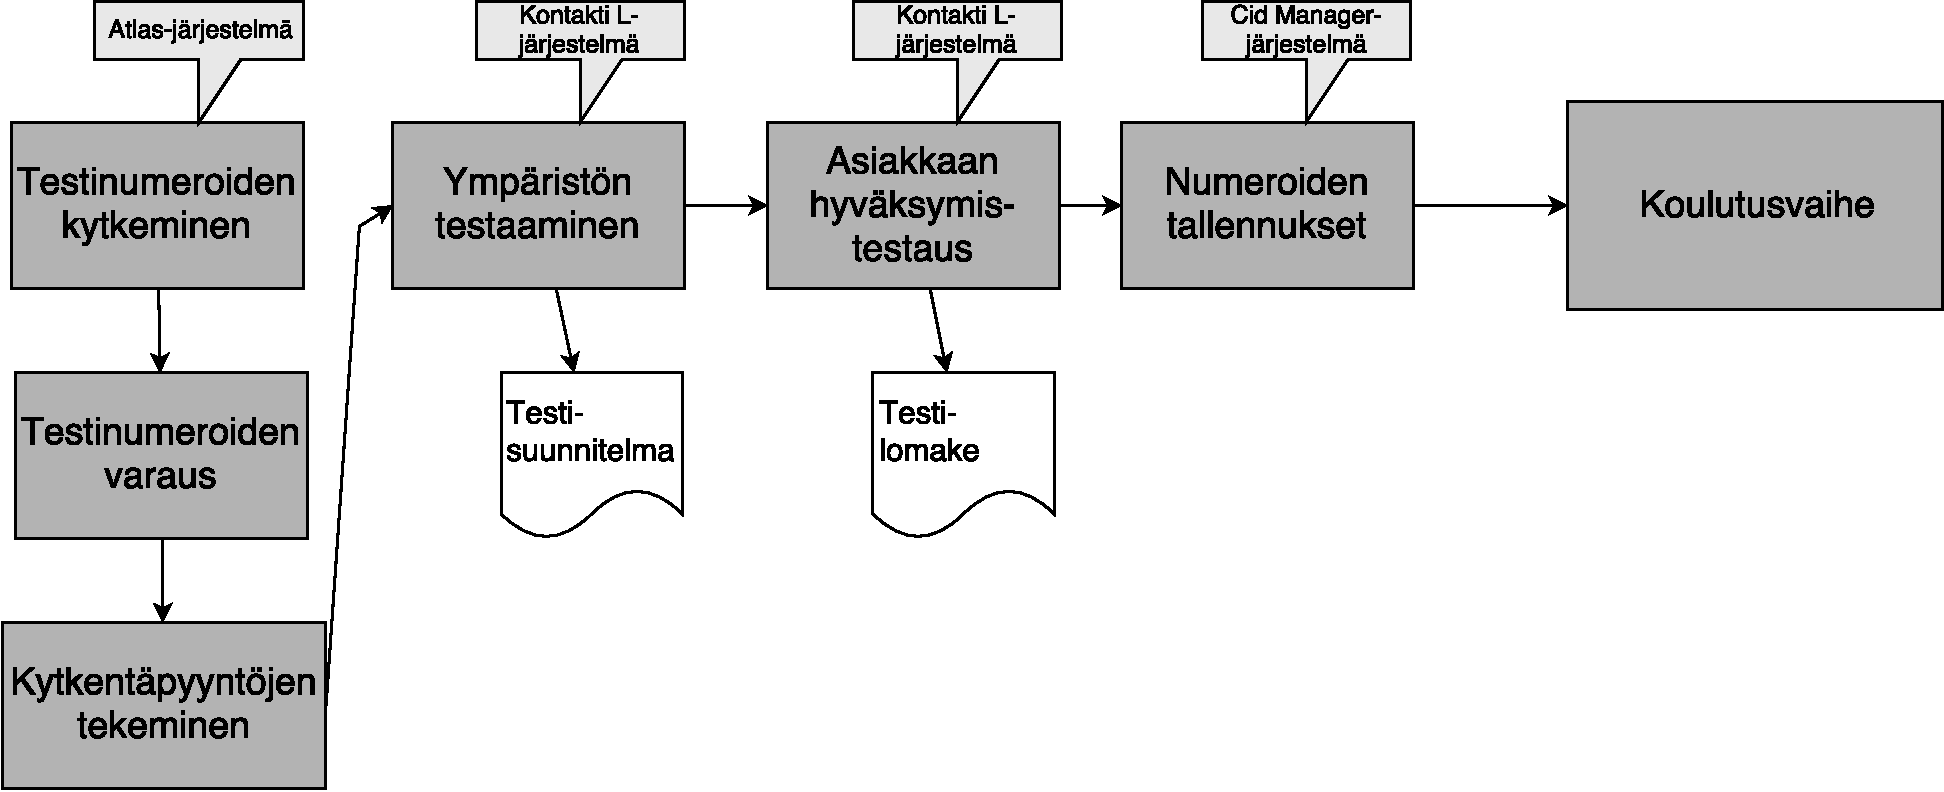
\includegraphics[scale=0.3]{images/Testaus.pdf}
    \caption{Kontakti L:n asiakasprosessin testausvaihe.}
    \label{fig:testaus}
\end{figure}

Puhesuunnittelija ja Telian järjestelmäasiantuntijat testaavat Kontakti L-järjestelmän toimintaa testisuunnitelman mukaisesti. Tämän jälkeen asiakkaalle ilmoitetaan järjestelmän olevan valmis hyväksymistestausta varten. Asiakas testaa järjestelmää Telian testilomakkeen avulla, ja kun järjestelmä todetaan vaatimuksia vastaavaksi, kuittaa asiakas sen toimitusprojektille. \\

Järjestelmän ollessa valmiina seutraavaa vaihetta varten, kytketään tuotannon numerot valmiiksi odottamaan koulutus- ja käyttöönottovaihetta.\\

\textbf{Koulutusvaihe}\\

%Vaiheen kesto on arvioitu olevan noin 1 kuukausi.\\

Kuvassa \ref{fig:koulutus} ilmenee koulutusvaiheen kulku. Koulutusvaihe alkaa kun kouluttaja käy sopimuksen läpi projektipäällikön tai toimitusvastaavan kanssa. Asiakkaan kanssa tehdystä sopimuksesta ilmenee mitä koulutuksista on sovittu asiakkaan kanssa.

\begin{figure}[!h]
    \centering
    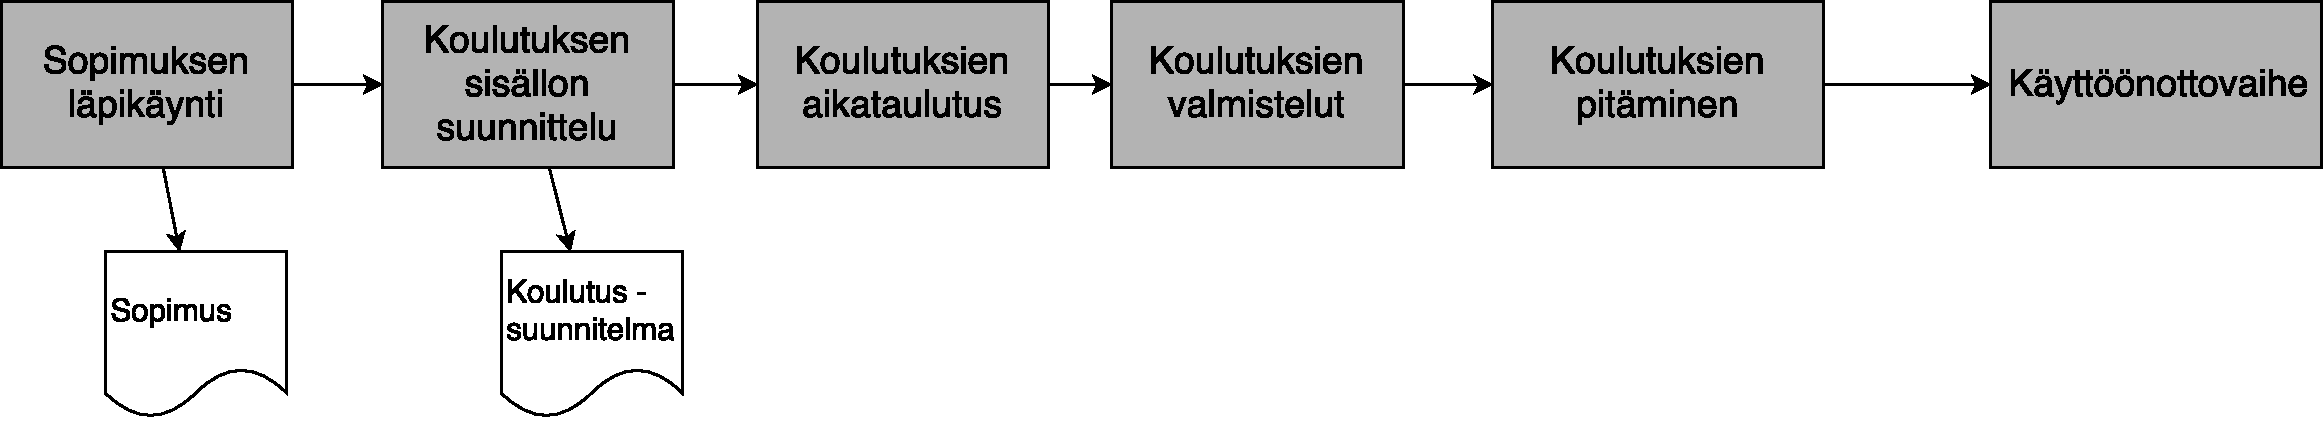
\includegraphics[scale=0.3]{images/koulutukset.pdf}
    \caption{Kontakti L:n asiakasprosessin koulutusvaihe.}
    \label{fig:koulutus}
\end{figure}

Sopimuksen perusteella kouluttaja suunnittelee koulutuksen sisällön ja tekee tästä kirjallisen suunnitelman. Koulutuksen sisällön ollessa selvillä, aikatauluttaa kouluttaja yhdessä projektipäällikön ja toimitusvastaavan kanssa tarvittavien koulutusten ajankohdan.\\

Kouluttaja tyypillisesti valmistelee koulutusta asiakkaan tarpeen mukaan, ja koulutus voidaan järjestää joko Telian tiloissa tai asiakkaalla. Kouluttaja pitää koulutukset suunnitelman mukaan. Järjestelmän käyttäjien ollessa valmiita ottamaan järjestelmä jokapäiväiseen käyttöön, alkaa käyttöönottovaihe.\\

\textbf{Käyttöönottovaihe}\\

%Vaiheen kesto on arvioitu olevan noin 1 kuukausi.\\

Käyttöönottovaihe on esitetty kuvassa \ref{fig:kayttoonotto}. Käyttöönottovaihe alkaa Kontakti L-järjestelmän siirtämisellä tuotantoon. Tämä tarkoittaa sitä, että ylläpito ja käyttö-prosessin aikaiset ohjeistukset, toimintamallit ja vastuut ovat selvillä. Myös asiakkaalle on viestittävä miten käyttöönoton jälkeen toimitaan. 

\begin{figure}[!h]
    \centering
    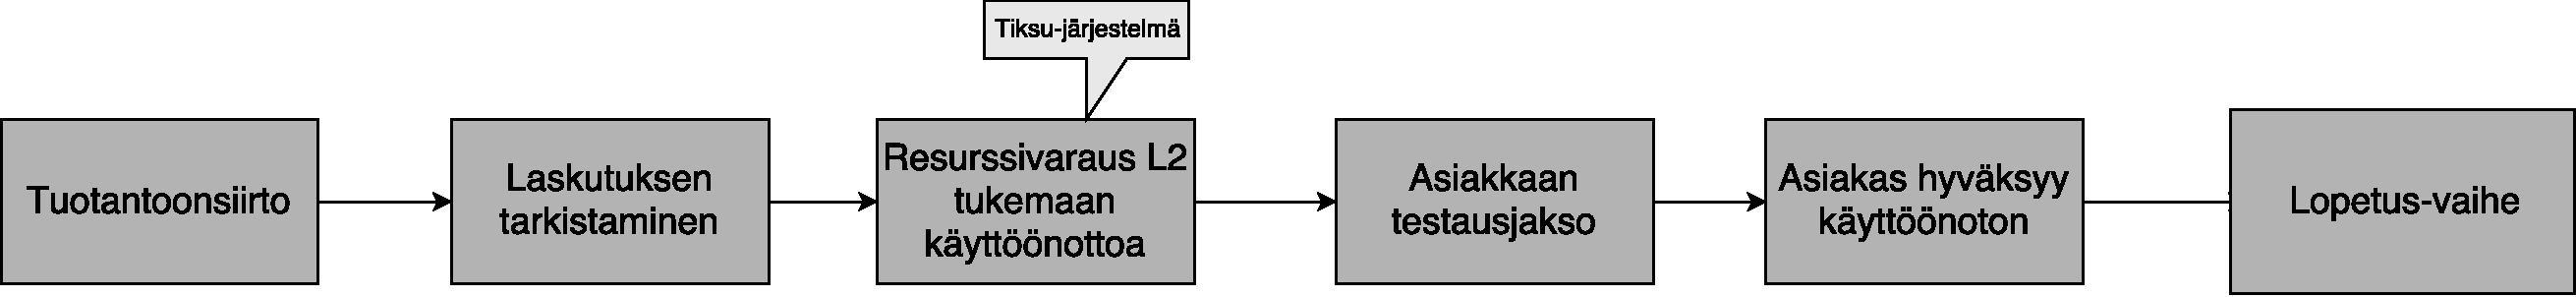
\includegraphics[scale=0.3]{images/kayttoonotto.pdf}
    \caption{Kontakti L:n asiakasprosessin käyttöönottovaihe.}
    \label{fig:kayttoonotto}
\end{figure}

Tuotantoonsiirron jälkeen toimitusvastaava varmistaa laskutusmallin ja asetusten oikeellisuuden. Tämän jälkeen hän varaa Tiksu-järjestelmästä resurssin tukemaan asiakasta Kontakti L-järjestelmän käyttöönotossa. Telian järjestelmäasiantuntija varaa tällöin aikaa käyttöönoton hetkellä jos ongelmatilanteita tulee eteen. Kontakti L-järjestelmän käyttöönotossa on myös testausjakso, jolloin rajatut toiminnallisuudet otetaan testikäyttöön. Asiakkaan hyväksyessä käyttöönoton, siirtyy asiakas Kontakti L-järjestelmän osalta seuraavaan asiakasprosessiin, eli ylläpito ja käyttö-prosessiin.\\

Telian näkökulmasta asiakasprosessin viimeinen vaihe on lopetusvaihe, jossa toimitusprojekti päätetään ja resurssit irrotetaan projektista. \\

\textbf{Lopetusvaihe}\\

Lopetusvaihe on esitetty kuvassa  \ref{fig:lopetus}. Lopetusvaiheen aluksi projektipäällikkö valmistelee toimitusprojektin loppuraportin, joka käydään läpi toimitusprojektin organisaation kanssa projektin päätöspalaverissa. Mukana on myös asiakas. Palaverin tarkoitus on käydä tehdyt asiat läpi ja myös mahdolliset asiat, joita ei toteutettu projektin aikana.\\

\begin{figure}[!h]
    \centering
    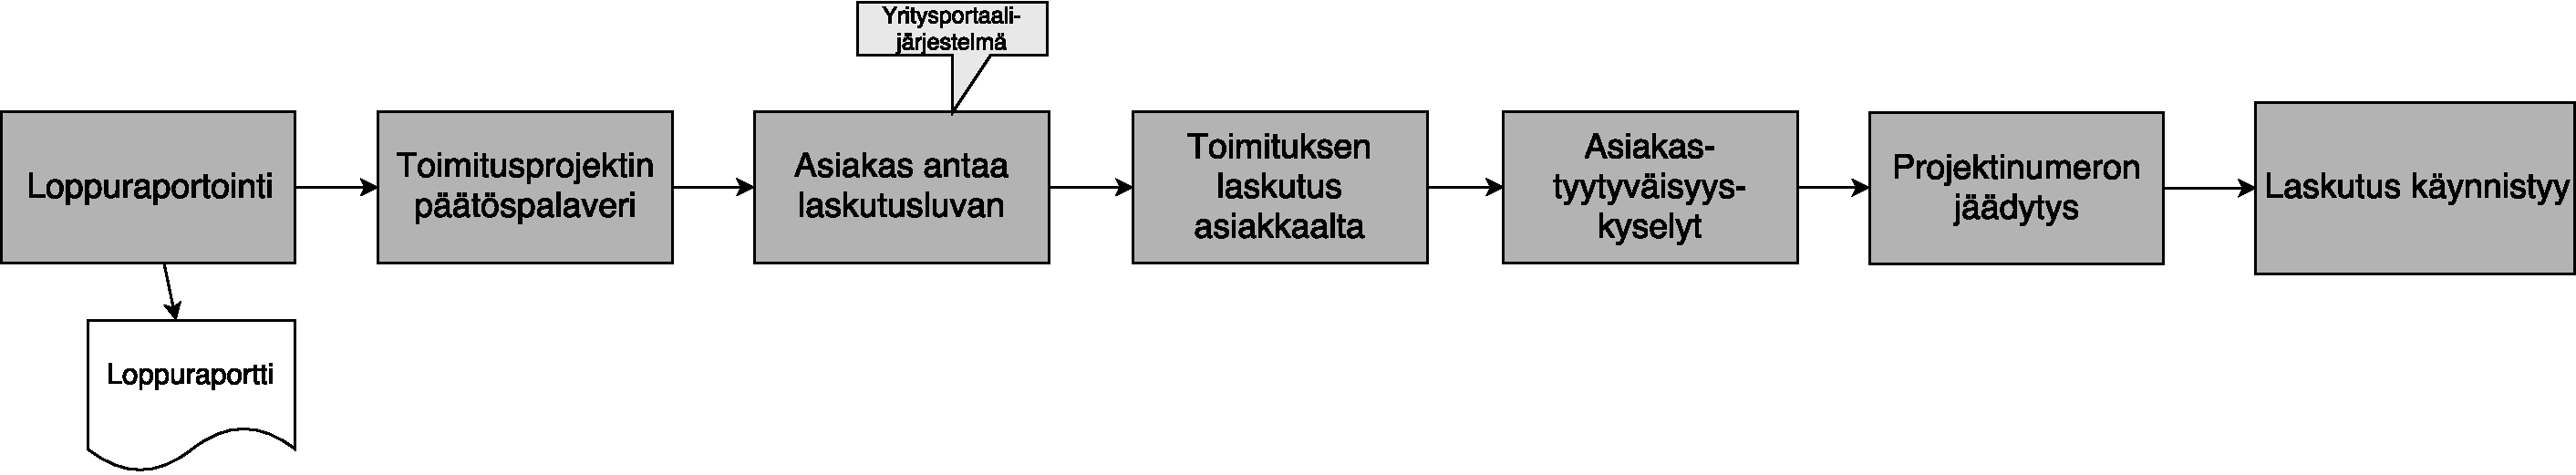
\includegraphics[scale=0.3]{images/lopetus.pdf}
    \caption{Kontakti L:n asiakasprosessin lopetusvaihe.}
    \label{fig:lopetus}
\end{figure}

Päätöspalaverin jälkeen projektipäällikkö pyytää asiakkaalta kirjallisesti luvan käynnistää Kontkati L:n laskutus. Tämän ohella projektipäällikkö myös laskuttaa asiakkaalta toimtusprojektin aikaiset työt.\\

Viimeisenä projektipäällikkö lähettää asiakastyytyväisyyskyselyn asiakkaan toimitusprojektissa mukana olleille henkilöille ja poistaa projektinumeron käytöstä. Kontakti L:n asiakasprosessi päättyy tilauksesta laskutukseen-prosessin osalta tähän.\\

\subsubsection{Esiin nousseet haasteet}

Prosessin rakennusvaiheen haasteet tavoitejärjestelmien ja vendorin osalta.


Käyttöönoton ongelmat usein joko lisäpalveluiden käyttöönoton haasteita tai ohjeiden epäselvyyksiin liittyviä. 


\textbf{Tilausvaiheessa esiin nousseet haasteet}\\

- Myyjä ei osaa täyttää paha-lomaketta ja jättää sen usein tekemättä\\
- Myyjällä ei ole tällöin tapaa viestiä siitä minkä palvelun hän on myynyt\\
- Myyjän on haastava viestiä eteenpäin mitä hän on myynyt\\

\textbf{Tilausten vastaanotto-vaiheessa esiin nousseet haasteet}\\

- Vaiheen läpi pääsee ilman PaHa-lomaketta, jolloin asiantuntijan täytyy selvittää joko myynnistä, projektitoimistolta tai tuotehallinnalta mitä tilaukselle tehdään.\\

Zylincin pystyttämisen automatisointi. Tilausvaiheen lomakkeet, myyjän vastuu, 

ODI-prosessin kuvaus.

Haettiin Ruotsin CallGuidea selkeästi halvempaa ja kevyempää IMS-yhteensopivaa ratkaisua, jolla voidaan korvata Merex/Mecm vaihteenhoitopalvelu ja kasvattaa markkinaosuutta ns. keskisegmentissä (joitain kymmeniä agentteja). Projekti taisi alkaa 2015 ja sopimusneuvotteluiden jälkeen tuotteistus/asiakasprosessin rakentaminen alkoi 2017 kesällä. Pilotoitiin kuitenkin jostain syystä yli sadan agentin asiakkaalla, jolla tuhansia kontakteja viikossa. Pilotti alkoi yli vuosi sitten ja teknisistä ongelmista johtuen laskutus ei ole alkanut vieläkään. Selkeästi halvemman hinnan ansiosta voitettu isoja toimijoiden kilpailutuksia. Useita alkuperäiseen haarukkaan kuuluneita asiakkaita jonossa, mutta toimitukset venyvät kaiken ajan kuluessa isojen toimitusten virittämiseen.

\subsection{Kappaleen yhteenveto}


\clearpage

\section{Havainnot}
%\section{Results}

Automaatioastetta voidaan ajatella nostettavan telian prosessiarkkitehtuurin ja toimintamallien kautta ja itse ohjelmiston rakennusvaiheiden automatisoinnilla. Tällä hetkellä kumpikaan osapuoli ei tue automaatiota. Eikä ohjelmisto sovellu helposti tavoitearkkitehtuuriin.

sisäisiä: laskutusjärjestelmä ei tue, järjestelmä lykätään käytännössä legacy platalle, yhteydet joita toimitetaan niin niiden toimitusta ei ole automatisoitu, numerointiin liittyvät aasiat ovat manuaalisia ja hitaita, toimitus projekti muokkaa tuotetta, prosessissa ei ole kontrollia, osaaminen zylincistä alkutekijöissä, toimitusprosessia ei määritelty lloppuun, automaatio-osaamista ei ole talossa tai zylincillä, ja aikataulupaineet johtavat hätäisiin ratkaisuihin. 
Ohjeslmisto: Rakennettu on-premises maailmaan, ei automaattista pystytystä, lisensointia, automaattisia päivityksiä, kehitys heikkoa,  mikä on zylincin kyky tuottaa ratkaisuja ajoissa? Minkälaista osaamista talossa on? Ei ainakaan automaatio-osaamista tai mindsettiä

Ratkaisu: ENSIN: päätetään liiketoiminnallinen tavoite jonka perusteella voidaan optimoida kokonaisuutta, eli tehdä päätöksiä mitä tehdään ja mitä ei. Virtaviivaistetaan toimintamalleja ensin ja katsotaan miten toimintamalleja voitaisiin määrämuotoistaa ja eliminoida, luodaan asiakkaalle enemmän mahdollisuuksia itsepalveluun koska sitä he toivovat, Tehdään päätöksiä mikä on se perusratkaisu jolla mennään ja saadaan asiakkaita, sitten katsotaan onko tuotteessa mahdollisuuksia automaatiolle.

Lähteekö tavoitteet automaatioon asiakkaiden tarpeista ja siten strategisista lähtökohsdista? Halutaanko sillä todella parantaa asiakkaan kokemusta vai tarjota samaa tehokkaammin?

Tutepäällikölle annettu tavoite 80prossasesta automaatiosta ei ole millään tavalla helposti ymmärrettävissä tai mitattavissa. Sillä ei ole liiketoiminnnallista selkeää tavoitetta. 

Se hetki kun päätetään mihin lähdetään ja mihin ei lähdetä määrittää identiteetin ja mittaa meidän arvot. Arvot ovat vain olemassa silloin kuin ne maksavat jotain. Tiedämmekö me ketä me olemme ja mihin me olemme menossa? Kyllä asiakaskeissit on isoja, ja niidne voittaminen on tärkeää. Mutta pitkitetäänkö jatkuvalla myönteisyydellä vain vääjäämätöntä? Olisiko syytä pysähtyä ja miettiä kaikki uudestaan, koska nykyisillä toimintamalleila ei ole tulevaisuutta. Jos meidän asiakkaat säilyvä't suurin piirtein samoina, ja me teemme aina asiakkaan vaatimusten mukaan, kehitymmekö me ollenkaan? Mutta jos me koemme että meidän täytyy voittaa kaikki asiakaskeissit mitä tulee vastaan esimerkiksi pelkät kilpailutukset, pitäisikö meidän etsiä asiakkaita muualtakin? Tiedämme mitä asiakkaamma haluavat, mutta mitä he oikeasti tarvitsevat? Menestyvässä liiketoiminnassa hävitään koko ajan kannattavaa kauppaa tahallaan, koska siihen on varaa. Mä haluan työskennellä sen tulevaisuuden eteen en nykyisyyden. Isoihin tavoitteisiin päästään yksi pieni askel kerrallaan, esim yksi päätös kerrallaan. Meidän täytyy johdonmukaisesti tehdä päätöksiä jotka ovat askel meidän tavoitetilaan.

Vastuu: Kaikilla on mahdollisuus keskeyttää tuotantolinja ja nostaa lippu pystyyn -> vastuu. Asiat vain tapahtuvat tai näin ollaan aina tehty, en tiedä kuka näistä päättää? -> ei vastuuta.
%% Huomaa seuraavassa kappaleessa lainausmerkkien ulkopuolella piste, 
%% koska piste ei lopeta lainattua tekstinpätkää.
%% Jos lainattu tekstinpätkä loppuu välimerkkiin, tulee välimerkki
%% lainausmerkkien sisälle: 
%% "Et tu, Brute?" sanoi Caesar kuollessaan.
Tutkimustuloksien merkitystä on aina syytä arvioida ja tarkastella
kriittisesti.  Joskus tarkastelu voi olla tässä osassa, mutta se
voidaan myös jättää viimeiseen osaan, jolloin viimeisen osan nimeksi
tulee >>Tarkastelu>>. Tutkimustulosten merkitystä voi arvioida myös
>>Johtopäätökset>>-otsikon alla viimeisessä osassa. 

Tässä osassa on syytä myös arvioida tutkimustulosten luotettavuutta.
Jos tutkimustulosten merkitystä arvioidaan >>Tarkastelu>>-osassa,
voi luotettavuuden arviointi olla myös siellä. 

\clearpage

\section{Tutkimuskysymyksiin vastaaminen}

\section{Yhteenveto}
%\section{Summary} 

Opinnäytteen tekijä vastaa siitä, että opinnäyte on tässä dokumentissa
ja opinnäytteen tekemistä käsittelevillä luennoilla sekä
harjoituksissa annettujen ohjeiden mukainen muotoseikoiltaan,
rakenteeltaan ja ulkoasultaan.



\clearpage
%% Lähdeluettelo
%%
%% \phantomsection varmistaa, että hyperref-paketti latoo hypertekstilinkit
%% oikein.
%%
%% The \phantomsection command is nessesary for hyperref to jump to the 
%% correct page, in other words it puts a hyper marker on the page.

\phantomsection
%\addcontentsline{toc}{section}{Viitteet}
%\addcontentsline{toc}{section}{References}
%%\begin{thebibliography}{99}
\bibliography{lahteet}

%% Alla pilkun jälkeen on pakotettu oikea väli \<välilyönti>-merkeillä.

%%\end{thebibliography}

%% Liitteet 
\appendix 
\clearpage
%% Lisää tekstin "Liitteet" sisällysluetteloon
%%
%% Adds the word "Appendices" to the table of contents
\addtocontents{toc}{\protect\contentsline{section}{Liiteet}{}{appendix}}
%\addtocontents{toc}{\protect\contentsline{section}{Appendices}{}{appendix}}

\section{Esimerkki liitteestä\label{LiiteA}}
%% Liitteiden kaavat, taulukot ja kuvat numeroidaan omana kokonaisuutenaan
%%
%% Equations, tables and figures have their own numbering in Appendices
\renewcommand{\theequation}{A\arabic{equation}}
\setcounter{equation}{0}  
\renewcommand{\thefigure}{A\arabic{figure}}
\setcounter{figure}{0}
\renewcommand{\thetable}{A\arabic{table}}
\setcounter{table}{0}

Liitteet eivät ole opinnäytteen kannalta välttämättömiä ja 
opinnäytteen tekijän on 
kirjoittamaan ryhtyessään hyvä ajatella pärjäävänsä ilman liitteitä.
Kokemattomat kirjoittajat, jotka ovat huolissaan
tekstiosan pituudesta, paisuttavat turhan 
helposti liitteitä pitääkseen tekstiosan pituuden annetuissa rajoissa.
Tällä tavalla ei synny hyvää opinnäytettä.   

Liite on itsenäinen kokonaisuus, vaikka se täydentääkin tekstiosaa.
Liite ei siten ole pelkkä listaus, kuva tai taulukko, vaan 
liitteessä selitetään aina sisällön laatu ja tarkoitus. 

Liitteeseen voi laittaa esimerkiksi listauksia. Alla on 
listausesimerkki tämän liitteen luomisesta. 

%% Verbatim-ympäristö ei muotoile tai tavuta tekstiä. Fontti on monospace.
%% Verbatim-ympäristön sisällä annettuja komentoja ei LaTeX käsittele. 
%% Vasta \end{verbatim}-komennon jälkeen jatketaan käsittelyä.
\begin{verbatim}
	\clearpage
	\appendix
	\addcontentsline{toc}{section}{Liite A}
	\section*{Liite A}
	...
	\thispagestyle{empty}
	...
	tekstiä
	...
	\clearpage
\end{verbatim}

Kaavojen numerointi muodostaa liitteissä oman kokonaisuutensa:
\begin{eqnarray}
d \wedge A  &=& F, \label{liitekaava1}\\
d \wedge F  &=& 0. \label{liitekaava2}
\end{eqnarray}


\clearpage
\section{Toinen esimerkki liitteestä\label{LiiteB}}

%% Liitteiden kaavat, taulukot ja kuvat numeroidaan omana kokonaisuutenaan
%%
%% Equations, tables and figures have their own numbering in Appendices
\renewcommand{\theequation}{B\arabic{equation}}
\setcounter{equation}{0}  
\renewcommand{\thefigure}{B\arabic{figure}}
\setcounter{figure}{0}
\renewcommand{\thetable}{B\arabic{table}}
\setcounter{table}{0}

Liitteissä voi myös olla kuvia, jotka
eivät sovi leipätekstin joukkoon:
%% Ympäristön figure parametrit htb pakottavat
%% kuvan tähän, eikä LaTeX yritä siirrellä niitä
%% hyväksi katsomaansa paikkaan. 
%% Ympäristöä center voi käyttää \centering-
%% komennon sijaan
%%
%% Example of a figure, note the use of htb parameters which force
%% the figure to be inserted here
\begin{figure}[htb]
\begin{center}
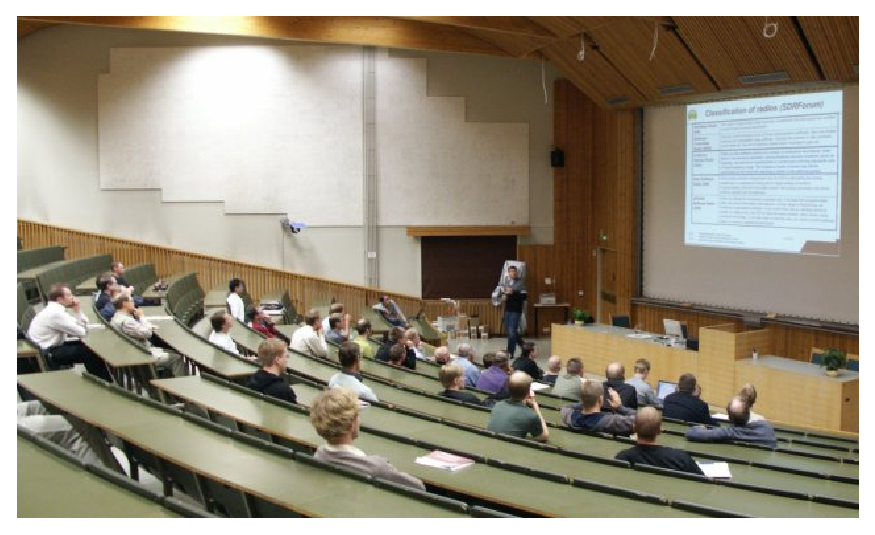
\includegraphics[height=8cm]{kuva2}
\end{center}
\caption{Kuvateksti, jossa on liitteen numerointi \label{liitekuva}}
\end{figure}
%%
Liitteiden taulukoiden numerointi on kuvien ja kaavojen kaltainen:
\begin{table}[htb]
\caption{Taulukon kuvateksti. \label{liitetaulukko}}
\begin{center}
\fbox{
\begin{tabular}{lp{0.5\linewidth}}
9.00--9.55  & Käytettävyystestauksen tiedotustilaisuus (osanottajat
ovat saaneet sähköpostitse valmistautumistehtävät, joten tiedotustilaisuus
voidaan pitää lyhyenä).\\
9.55--10.00 & Testausalueelle siirtyminen
\end{tabular}}
\end{center}
\end{table}
Kaavojen numerointi muodostaa liitteissä oman kokonaisuutensa:
\begin{eqnarray}
T_{ik} &=& -p g_{ik} + w u_i u_k + \tau_{ik},  \label{liitekaava3} \\
n_i    &=& n u_i + v_i.                        \label{liitekaava4}
\end{eqnarray}

\end{document}
